\documentclass[12pt,a4paper,oneside]{report}
\input{glyphtounicode}
\pdfgentounicode=1

% ==============================================================================
% GÓI HỖ TRỢ TIẾNG VIỆT VÀ ĐỊNH DẠNG TRANG IN
% ==============================================================================
\usepackage[utf8]{vietnam}
\usepackage[left=3.5cm,right=2.0cm,top=2.5cm,bottom=2.5cm]{geometry}
\usepackage{setspace}
\onehalfspacing % Giãn dòng 1.5 theo quy chuẩn luận văn

% ==============================================================================
% CÁC GÓI TOÁN HỌC, ĐỒ HỌA VÀ BẢNG BIỂU
% ==============================================================================
\usepackage{amsmath,amssymb,amsthm}
\usepackage{graphicx}
\graphicspath{{figures/}}
\usepackage{booktabs}
\usepackage{tabularx}
\usepackage{longtable}
\usepackage{multirow}
\usepackage{array}
\usepackage{float}
\usepackage{caption}
\usepackage{subcaption}
\usepackage{enumitem}

% ==============================================================================
% ĐỊNH DẠNG MÃ NGUỒN VÀ THUẬT TOÁN
% ==============================================================================
\usepackage{listings}
\usepackage{xcolor}
\usepackage{algorithm}
\usepackage{algpseudocode}

\definecolor{codegreen}{rgb}{0,0.6,0}
\definecolor{codegray}{rgb}{0.5,0.5,0.5}
\definecolor{codepurple}{rgb}{0.58,0,0.82}
\definecolor{backcolour}{rgb}{0.96,0.96,0.96}

\lstdefinestyle{mystyle}{
    backgroundcolor=\color{backcolour},   
    commentstyle=\color{codegreen},
    keywordstyle=\color{magenta},
    numberstyle=\tiny\color{codegray},
    stringstyle=\color{codepurple},
    basicstyle=\ttfamily\footnotesize,
    breakatwhitespace=false,         
    breaklines=true,                 
    captionpos=b,                    
    keepspaces=true,                 
    numbers=left,                    
    numbersep=5pt,                  
    showspaces=false,                
    showstringspaces=false,
    showtabs=false,                  
    tabsize=2
}
\lstset{style=mystyle}

% ==============================================================================
% ĐỊNH DẠNG TIÊU ĐỀ CHƯƠNG MỤC VÀ HEADER/FOOTER
% ==============================================================================
\usepackage{titlesec}
\titleformat{\chapter}[display]
  {\normalfont\bfseries\Large\centering}
  {\MakeUppercase{\chaptertitlename}\ \thechapter}{15pt}{\Large\MakeUppercase}
\titlespacing*{\chapter}{0pt}{-20pt}{25pt}

\usepackage{fancyhdr}
\pagestyle{fancy}
\setlength{\headheight}{17pt}
\fancyhf{}
\renewcommand{\chaptermark}[1]{\markboth{\chaptertitlename\ \thechapter.\ #1}{}}
\fancyhead[L]{\small\leftmark}
\fancyhead[R]{\small ĐATN}
\fancyfoot[C]{\thepage}
\renewcommand{\headrulewidth}{0.5pt}
\renewcommand{\footrulewidth}{0pt}

% ==============================================================================
% HYPERREF VÀ LIÊN KẾT
% ==============================================================================
\usepackage[unicode,colorlinks=true,linkcolor=blue,citecolor=red,urlcolor=teal]{hyperref}

% Định nghĩa môi trường Bất biến Thiết kế / Định nghĩa / Tiên đề
\newtheorem{invariant}{Bất biến Thiết kế}[chapter]
\newtheorem{definition}{Định nghĩa}[chapter]
\newtheorem{axiom}{Tiên đề}[chapter]

\emergencystretch=3em

\begin{document}

% ==============================================================================
% PHẦN ĐẦU (FRONTMATTER): Bìa, Lời cam đoan, Lời cảm ơn, Mục lục...
% ==============================================================================
\pagenumbering{roman}
% ==============================================================================
% TRANG BÌA CHÍNH (TITLE PAGE)
% ==============================================================================
\begin{titlepage}
\begin{center}
    \textbf{\large BỘ GIÁO DỤC VÀ ĐÀO TẠO}\\[0.25cm]
    \textbf{\large TRƯỜNG ĐẠI HỌC PHENIKAA}\\[0.25cm]
    \textbf{\large KHOA KHOA HỌC MÁY TÍNH}\\[0.8cm]

    \vspace{0.8cm} % Chỗ chèn Logo Trường Đại học Phenikaa (nếu có: \includegraphics[width=0.25\textwidth]{figures/logo.png})

    \textbf{\Large BÁO CÁO ĐỒ ÁN TỐT NGHIỆP ĐẠI HỌC}\\[0.3cm]
    \textbf{\large NGÀNH: KHOA HỌC MÁY TÍNH}\\[0.2cm]
    \textbf{\large CHUYÊN NGÀNH: TRÍ TUỆ NHÂN TẠO}\\[0.8cm]

    \begin{onehalfspace}
        {\bfseries\large NGHIÊN CỨU VÀ XÂY DỰNG TRÒ CHƠI TRINH THÁM GIẢI ĐỐ TRÊN NỀN TẢNG WEB, ỨNG DỤNG MÔ HÌNH NGÔN NGỮ LỚN (LLM) ĐỂ SINH TỰ ĐỘNG CÁC BỘ HỒ SƠ VỤ ÁN CÓ TÍNH LOGIC VÀ NHẤT QUÁN}\\[0.35cm]
        {\normalsize\textbf{Hướng tiếp cận Neuro-Symbolic kết hợp Hệ đa tác tử và Bộ kiểm định hình thức}}\\[0.25cm]
        {\small\textit{(Research and Development of a Web-Based Detective Puzzle Game Using Large Language Models for Procedural Generation of Logical and Consistent Case Dossiers: A Neuro-Symbolic Multi-Agent Approach)}}
    \end{onehalfspace}

    \vfill

    \begin{table}[h]
        \centering
        \begin{tabular}{ll}
            \textbf{Sinh viên thực hiện:} & \textbf{Nguyễn Ngọc Công Anh} \\
            \textbf{Mã số sinh viên:}     & \textbf{22010201} \\
            \textbf{Lớp:}                & \textbf{K16-KHMT} \\
            \textbf{Cán bộ hướng dẫn:}    & \textbf{TS. Nguyễn Văn Tánh}
        \end{tabular}
    \end{table}

    \vspace{0.4cm}
    \textbf{\large HÀ NỘI – NĂM 2026}
\end{center}
\end{titlepage}

% ==============================================================================
% LỜI CAM ĐOAN
% ==============================================================================
\newpage
\chapter*{LỜI CAM ĐOAN}
\addcontentsline{toc}{chapter}{LỜI CAM ĐOAN}

Tôi xin cam đoan bản báo cáo đồ án tốt nghiệp với đề tài \textit{``Nghiên cứu và xây dựng trò chơi trinh thám giải đố trên nền tảng Web, ứng dụng mô hình ngôn ngữ lớn (LLM) để sinh tự động các bộ hồ sơ vụ án có tính logic và nhất quán''} là công trình nghiên cứu độc lập của riêng tôi dưới sự định hướng và hướng dẫn khoa học trực tiếp của TS. Nguyễn Văn Tánh.

Toàn bộ các số liệu đo đạc thực nghiệm, kết quả thống kê benchmark và mã nguồn hệ thống được trình bày trong luận văn này là trung thực, phản ánh đúng kết quả thu được trong quá trình nghiên cứu và cài đặt. Mọi sự kế thừa từ các công trình nghiên cứu trước đây, các thư viện mã nguồn mở, cũng như các tài liệu tham khảo khoa học đều được trích dẫn và ghi nhận tường minh theo đúng chuẩn mực liêm chính học thuật quốc tế. Tôi xin chịu hoàn toàn trách nhiệm trước Hội đồng chấm tốt nghiệp và Nhà trường về tính nguyên bản của công trình này.

\vspace{1.5cm}
\begin{flushright}
    \textit{Hà Nội, ngày 17 tháng 11 năm 2026}\\[0.2cm]
    \textbf{Sinh viên thực hiện}\\[1.5cm]
    \textbf{Nguyễn Ngọc Công Anh}
\end{flushright}

% ==============================================================================
% LỜI CẢM ƠN
% ==============================================================================
\newpage
\chapter*{LỜI CẢM ƠN}
\addcontentsline{toc}{chapter}{LỜI CẢM ƠN}

Để có thể hoàn thành chương trình đào tạo ngành Khoa học máy tính tại Trường Đại học Phenikaa và hoàn thiện bản báo cáo đồ án tốt nghiệp này, tôi đã nhận được sự dạy bảo, hỗ trợ và động viên to lớn từ các Thầy Cô giáo, gia đình và bạn bè.

Lời đầu tiên, tôi xin bày tỏ lòng biết ơn sâu sắc và chân thành nhất tới \textbf{TS. Nguyễn Văn Tánh}, người Thầy đã tận tâm hướng dẫn, truyền thụ phương pháp tư duy khoa học, định hướng kiến trúc hệ thống và luôn đưa ra những câu hỏi phản biện nghiêm khắc giúp tôi trưởng thành đáng kể cả về năng lực học thuật lẫn tư duy kỹ thuật trong suốt quá trình thực hiện đồ án.

Tôi xin chân thành cảm ơn Ban Giám hiệu Trường Đại học Phenikaa, Ban Chủ nhiệm Khoa Khoa học máy tính cùng toàn thể quý Thầy Cô giáo đã truyền thụ những nền tảng tri thức quý báu về Toán học, Cấu trúc dữ liệu và giải thuật, Học máy, Xử lý ngôn ngữ tự nhiên và Kỹ nghệ phần mềm trong suốt bốn năm học tập dưới mái trường.

Con xin bày tỏ lòng biết ơn sâu nặng tới Bố Mẹ và gia đình, những người luôn là điểm tựa tinh thần vững chắc, tạo mọi điều kiện tốt nhất để con yên tâm học tập và theo đuổi định hướng nghiên cứu khoa học.

Cuối cùng, tôi xin gửi lời cảm ơn tới những người bạn đồng môn đã luôn đồng hành, chia sẻ kinh nghiệm, hỗ trợ kiểm thử hệ thống và thảo luận chuyên môn trong suốt thời gian qua.

\vspace{1.5cm}
\begin{flushright}
    \textit{Hà Nội, tháng 11 năm 2026}\\[0.2cm]
    \textbf{Sinh viên}\\[1.5cm]
    \textbf{Nguyễn Ngọc Công Anh}
\end{flushright}

% ==============================================================================
% TÓM TẮT ĐỒ ÁN (TIẾNG VIỆT VÀ TIẾNG ANH)
% ==============================================================================
\newpage
\chapter*{TÓM TẮT ĐỒ ÁN}
\addcontentsline{toc}{chapter}{TÓM TẮT ĐỒ ÁN}

Sự phát triển nhanh chóng của các mô hình ngôn ngữ lớn (LLM) mở ra tiềm năng đáng kể cho lĩnh vực sinh nội dung thủ tục (PCG) trong trò chơi điện tử. Tuy nhiên, việc ứng dụng LLM nguyên khối vào thể loại trò chơi giải đố trinh thám suy diễn gặp phải nhiều rào cản bản chất như hiện tượng ảo giác nhân quả, mâu thuẫn mốc thời gian tử vong sinh học và vi phạm nguyên tắc trinh thám công bằng theo mười điều răn của Ronald Knox. Cơ chế sinh tự quy hồi theo xác suất của LLM không đủ để bảo đảm tính nhất quán của chuỗi suy luận hình thức nhiều bước.

Đồ án này đề xuất một khung kiến trúc lai Neuro-Symbolic kết hợp chuỗi 4 tác tử tuần tự (\texttt{OutlineAgent}, \texttt{CharacterAgent}, \texttt{ClueAgent}, \texttt{DeductionAgent}) với bộ kiểm định quy tắc tất định. Hệ thống tách biệt rõ ràng giữa dữ liệu chân lý gốc với dữ liệu trình bày cho người chơi, tích hợp phương trình làm lạnh thi thể hai hàm mũ của Henssge (giải số bằng phương pháp chia đôi) để khóa cứng cửa sổ thời gian tử vong (TOD), đồng thời sử dụng biểu diễn đồ thị hai phía để kiểm tra tính duy nhất của thủ phạm và sự tồn tại của manh mối bẻ gãy ngoại phạm. Khi phát hiện sai phạm, cơ chế sửa lỗi cục bộ định tuyến tín hiệu chẩn đoán tới đúng tác tử liên quan với độ phức tạp ngữ cảnh hằng số $\mathcal{O}(1)$ nhằm tránh tái sinh toàn bộ hồ sơ ($\mathcal{O}(N)$). Hệ thống vận hành trên kiến trúc dịch vụ Web RESTful API (\texttt{FastAPI}, giao thức HTTP/JSON, bảo mật HMAC-SHA256) kết hợp lưu trữ SQLite (SQLAlchemy 2.0) và giao diện điều tra đa nền tảng trên Unity 6 kết xuất bằng đường ống kết xuất phổ quát (URP) hỗ trợ chuẩn WebGL trình duyệt và máy trạm.

Kết quả thực nghiệm qua 30 phiên thử nghiệm độc lập trên 3 dòng mô hình (\texttt{gh/gpt-4o-mini}, \texttt{gh/gpt-4o}, \texttt{ollama/gemma4:31b-cloud}) cho thấy toàn bộ 30 kịch bản đạt \textbf{100\% tỷ lệ hợp lệ cú pháp JSON} dưới chuẩn Pydantic v2, nâng tỷ lệ vượt qua kiểm định logic lên mức \textbf{90\% -- 100\%}, chặn lọc được lỗi tham chiếu thực thể phát sinh ở \texttt{gh/gpt-4o}, và giữ độ trễ trung vị P50 ở mức \textbf{10.73s -- 10.88s} đối với hai mô hình phản hồi nhanh (\textbf{19.53s} đối với \texttt{gh/gpt-4o}).

\vspace{0.5cm}
\noindent\textbf{Từ khóa:} \textit{Mô hình ngôn ngữ lớn, Hệ đa tác tử, Neuro-Symbolic AI, Sinh nội dung thủ tục, Trò chơi trinh thám, Mô hình nhiệt Henssge, Đồ thị hai phía, Pydantic v2, Unity URP.}

\newpage
\chapter*{ABSTRACT}
\addcontentsline{toc}{chapter}{ABSTRACT}

The rapid evolution of Large Language Models (LLMs) presents substantial opportunities for Procedural Content Generation (PCG) in interactive video games. However, applying monolithic LLMs to deductive mystery games encounters fundamental obstacles, including causal hallucinations, biological post-mortem interval contradictions, and frequent violations of classic ``Fair-Play Mystery'' conventions (Knox's Decalogue). The probabilistic autoregressive nature of LLMs cannot guarantee strict formal consistency across multi-hop deductive inference chains on its own.

This thesis presents a \textbf{Neuro-Symbolic Hybrid Framework} that combines a 4-stage sequential Multi-Agent pipeline (\texttt{OutlineAgent}, \texttt{CharacterAgent}, \texttt{ClueAgent}, \texttt{DeductionAgent}) with a deterministic symbolic rule-based validator engine. The architecture decouples the underlying ground-truth state from player-facing dossier presentation and verification. It incorporates Henssge's two-exponential forensic cooling model solved numerically via the bisection method to enforce post-mortem Time of Death ($TOD$) windows as physical invariants, while using bipartite graph modeling to verify culprit uniqueness and alibi-breaking clue reachability. When constraint violations are detected, a localized patch repair mechanism isolates the responsible component with $\mathcal{O}(1)$ repair-context complexity rather than regenerating the entire dossier ($\mathcal{O}(N)$). The complete system operates on a distributed Web service architecture using a Python FastAPI RESTful API (HTTP/JSON, HMAC-SHA256) backed by SQLite (SQLAlchemy 2.0 WAL) and a cross-platform Unity 6 URP 2D corkboard client targeting both browser WebGL and standalone runtime environments.

Empirical evaluation across 30 independent trials benchmarking three representative models (\texttt{gh/gpt-4o-mini}, \texttt{gh/gpt-4o}, \texttt{ollama/gemma4:31b-cloud}) achieves \textbf{100.0\% syntactic schema validity} under Pydantic v2, maintains \textbf{90.0\% -- 100.0\% logic validation pass rates} while reliably flagging referential hallucination errors before client delivery, and records median P50 end-to-end generation latencies of \textbf{10.73s -- 10.88s} on fast open-weights and compact commercial models (\textbf{19.53s} on \texttt{gh/gpt-4o}).

\vspace{0.5cm}
\noindent\textbf{Keywords:} \textit{Large Language Models, Multi-Agent Systems, Neuro-Symbolic AI, Procedural Content Generation, Detective Mystery Games, Henssge Cooling Model, Bipartite Graph Solvability, Pydantic v2, Unity URP.}

% ==============================================================================
% MỤC LỤC VÀ DANH MỤC DANH SÁCH
% ==============================================================================
\newpage
\tableofcontents

\newpage
\listoftables
\addcontentsline{toc}{chapter}{DANH MỤC BẢNG BIỂU}

\newpage
\listoffigures
\addcontentsline{toc}{chapter}{DANH MỤC HÌNH VẼ}

% ==============================================================================
% DANH MỤC TỪ VIẾT TẮT
% ==============================================================================
\newpage
\chapter*{DANH MỤC CÁC TỪ VIẾT TẮT}
\addcontentsline{toc}{chapter}{DANH MỤC CÁC TỪ VIẾT TẮT}

{\small
\begin{longtable}{c l p{5.5cm} p{5.8cm}}
\toprule
\textbf{STT} & \textbf{Ký hiệu} & \textbf{Thuật ngữ tiếng Anh} & \textbf{Giải nghĩa tiếng Việt} \\
\midrule
\endfirsthead
\toprule
\textbf{STT} & \textbf{Ký hiệu} & \textbf{Thuật ngữ tiếng Anh} & \textbf{Giải nghĩa tiếng Việt} \\
\midrule
\endhead
\bottomrule
\endfoot
1  & \textbf{ACID}    & Atomicity, Consistency, Isolation, Durability & Tính nguyên tử, nhất quán, cô lập, bền vững \\
2  & \textbf{ADR}     & Architecture Decision Record                  & Bản ghi quyết định kiến trúc \\
3  & \textbf{AI}      & Artificial Intelligence                       & Trí tuệ nhân tạo \\
4  & \textbf{API}     & Application Programming Interface             & Giao diện lập trình ứng dụng \\
5  & \textbf{CoT}     & Chain-of-Thought                              & Kỹ thuật suy luận theo chuỗi \\
6  & \textbf{FSM}     & Finite State Machine                          & Máy trạng thái hữu hạn \\
7  & \textbf{GPT}     & Generative Pre-trained Transformer            & Mô hình Transformer tạo sinh tiền huấn luyện \\
8  & \textbf{HMAC}    & Hash-based Message Authentication Code        & Mã xác thực thông điệp dựa trên hàm băm \\
9  & \textbf{HTTP}    & Hypertext Transfer Protocol                   & Giao thức truyền tải siêu văn bản \\
10 & \textbf{JSON}    & JavaScript Object Notation                    & Định dạng trao đổi dữ liệu văn bản có cấu trúc \\
11 & \textbf{LAN}     & Local Area Network                            & Mạng máy tính cục bộ \\
12 & \textbf{LLM}     & Large Language Model                          & Mô hình ngôn ngữ lớn \\
13 & \textbf{NPC}     & Non-Player Character                          & Nhân vật không phải người chơi \\
14 & \textbf{P50}     & 50th Percentile (Median)                      & Phân vị thứ 50 (Trung vị) \\
15 & \textbf{P95}     & 95th Percentile                               & Phân vị thứ 95 \\
16 & \textbf{PCG}     & Procedural Content Generation                 & Sinh nội dung theo thủ tục \\
17 & \textbf{PMI}     & Post-Mortem Interval                          & Khoảng thời gian sau tử vong \\
18 & \textbf{RAM}     & Random Access Memory                          & Bộ nhớ truy cập ngẫu nhiên \\
19 & \textbf{REST}    & Representational State Transfer               & Kiến trúc truyền trạng thái đại diện \\
20 & \textbf{SHA-256} & Secure Hash Algorithm 256-bit                 & Giải thuật băm an toàn 256-bit \\
21 & \textbf{TOD}     & Time of Death                                 & Cửa sổ thời gian tử vong \\
22 & \textbf{URP}     & Universal Render Pipeline                     & Đường ống kết xuất phổ quát trong Unity \\
23 & \textbf{WAL}     & Write-Ahead Logging                           & Cơ chế ghi nhật ký trước trong cơ sở dữ liệu \\
\end{longtable}
}


% ==============================================================================
% PHẦN NỘI DUNG CHÍNH (MAIN BODY)
% ==============================================================================
\newpage
\pagenumbering{arabic}
\setcounter{page}{1}

\chapter{TỔNG QUAN VÀ PHÁT BIỂU BÀI TOÁN}
\label{ch:introduction}

\section{Bối cảnh nghiên cứu và Tính cấp thiết}
\label{sec:intro_context}

Trong lịch sử hơn bốn thập kỷ phát triển của ngành công nghiệp trò chơi điện tử và khoa học máy tính ứng dụng trong giải trí tương tác, kỹ thuật sinh nội dung thủ tục (PCG\textsuperscript{16}) luôn được coi là một trong những trụ cột công nghệ then chốt \cite{summerville2018procedural}. Khởi nguồn từ những tựa game kinh điển như \textit{Rogue} (1980) hay \textit{NetHack} (1987), PCG cho phép các nhà phát triển sử dụng các thuật toán tất định hoặc ngẫu nhiên có kiểm soát (như nhiễu Perlin, phân rã không gian nhị phân, hay máy ôtômat tế bào) để kiến tạo nên các mê cung, địa hình và vị trí vật phẩm mà không cần sự can thiệp thủ công của con người \cite{short2017procedural}. Mục tiêu trọng tâm của PCG là gia tăng giá trị chơi lại của trò chơi, đồng thời cắt giảm chi phí sản xuất nội dung đồ họa và kịch bản.

Tuy nhiên, trong suốt nhiều thập kỷ, phạm vi áp dụng của PCG truyền thống chủ yếu dừng lại ở các nội dung mang tính cấu trúc không gian hình học hoặc các hệ thống nhiệm vụ đơn giản dựa trên văn phạm đồ thị. Khi bước vào địa hạt của nghệ thuật kể chuyện tương tác và đặc biệt là thể loại trò chơi trinh thám suy diễn, các thuật toán PCG cổ điển bộc lộ nhiều hạn chế. Một kịch bản trinh thám không đơn thuần là sự sắp đặt ngẫu nhiên của các căn phòng, mà là một mạng lưới quan hệ xã hội phức tạp, đan xen giữa động cơ tâm lý, các chứng cứ ngoại phạm có chủ đích và chuỗi nhân quả chặt chẽ kết nối từ hành vi phạm tội tới dấu vết tại hiện trường.

Sự phát triển nhanh chóng của các mô hình ngôn ngữ lớn (LLM\textsuperscript{12}) dựa trên kiến trúc Transformer \cite{vaswani2017attention} từ năm 2022 đã mở ra hướng tiếp cận mới cho ngành kỹ nghệ trò chơi. Nhờ quá trình tiền huấn luyện trên các kho ngữ liệu văn bản quy mô lớn, các mô hình tiên tiến hiện nay như mô hình Transformer tạo sinh tiền huấn luyện (GPT\textsuperscript{7}) \cite{achiam2023gpt4} hay Gemma \cite{gemmateam2024gemma} đã thể hiện năng lực xử lý ngôn ngữ tự nhiên tốt, khả năng nhập vai linh hoạt, mô tả văn cảnh giàu tính biểu cảm và thiết lập hội thoại nhân vật tự nhiên. Điều này thúc đẩy cộng đồng nghiên cứu trí tuệ nhân tạo (AI\textsuperscript{3}) hướng tới mục tiêu tự động hóa quy trình sáng tác các kịch bản trinh thám đa dạng, nơi mỗi phiên chơi là một vụ án độc lập được tạo sinh động.

Mặc dù vậy, khoảng cách từ một đoạn văn bản do LLM sinh ra có vẻ trôi chảy bề mặt đến một kịch bản trò chơi trinh thám thực sự có thể giải được vẫn là một thách thức khoa học lớn. Thể loại trinh thám suy diễn đòi hỏi tính toán logic hình thức nghiêm ngặt, nơi mọi mâu thuẫn thời gian dù chỉ vài phút, hay sai lệch vài độ C trong thân nhiệt thi thể, cũng đủ làm sụp đổ chuỗi suy luận của người chơi. Do đó, việc nghiên cứu một phương pháp tiếp cận lai kết hợp năng lực sáng tạo ngữ nghĩa của LLM với các cơ chế kiểm chứng toán học tất định là yêu cầu cấp thiết cả về mặt lý thuyết lẫn ứng dụng thực tiễn.

\section{Khoảng trống thực tiễn: Giới hạn của LLM trong Suy luận Hình thức}
\label{sec:intro_limitations}

Khi áp dụng phương pháp tạo sinh nguyên khối -- yêu cầu một mô hình ngôn ngữ lớn đơn lẻ sinh ra toàn bộ hồ sơ vụ án thông qua một câu lệnh duy nhất -- hệ thống thường gặp ba rào cản mang tính bản chất:

\subsection{Hiện tượng Ảo giác Nhân quả và Mâu thuẫn Thời gian}
Về mặt toán học, các LLM hiện đại vận hành như những bộ dự đoán token kế tiếp theo phân phối xác suất tự quy hồi:
\begin{equation}
    P(w_1, w_2, \dots, w_n) = \prod_{i=1}^n P(w_i \mid w_1, \dots, w_{i-1})
\end{equation}

Bản chất của cơ chế này là tối ưu hóa sự trôi chảy bề mặt và tính hợp lý thống kê của chuỗi văn bản, chứ không duy trì một mô hình trạng thái thế giới vật lý nhất quán bên trong \cite{marcus2020next}. Khi xử lý chuỗi suy luận nhân quả nhiều bước \cite{pearl2009causality}, các sai số xác suất nhỏ ở từng bước dễ tích lũy theo chiều dài văn bản, dẫn đến các mâu thuẫn phi lý:
\begin{itemize}[leftmargin=1.5cm]
    \item \textbf{Mâu thuẫn nhiệt học pháp y:} LLM có thể mô tả nạn nhân tử vong lúc 20:00 tối hôm trước, nhưng trong báo cáo khám nghiệm tử thi lúc 08:00 sáng hôm sau tại phòng $18^\circ\text{C}$ lại gán thân nhiệt thi thể là $36.5^\circ\text{C}$, vi phạm quy luật truyền nhiệt sinh học.
    \item \textbf{Mâu thuẫn không gian -- thời gian:} Một nghi phạm được mô tả có mặt tại quán cà phê cách hiện trường 30 km vào lúc 21:15, nhưng lời khai ở đoạn sau lại khẳng định nhân vật này trực tiếp có mặt tại hiện trường lúc 21:20.
\end{itemize}

\subsection{Vi phạm Nguyên tắc Trinh thám Công bằng}
Trong lịch sử văn học trinh thám cổ điển, vào năm 1929, học giả Ronald Knox đã công bố Mười điều răn của tiểu thuyết trinh thám (\textit{Knox's Decalogue}) theo nguyên tắc trinh thám công bằng (\textit{fair-play mystery}) \cite{knox1929ten}. Nguyên tắc cốt lõi của trinh thám công bằng quy định rằng người chơi phải được trao cơ hội bình đẳng với thám tử trong việc khám phá chân tướng vụ án:
\begin{enumerate}[label=(\roman*)]
    \item Toàn bộ các manh mối cần thiết để suy ra thủ phạm phải được trình bày tường minh trong hồ sơ vụ án;
    \item Không xuất hiện yếu tố siêu nhiên, chất độc giả tưởng chưa từng được khoa học biết đến, hay sự trùng hợp ngẫu nhiên vô căn cứ;
    \item Tồn tại chuỗi chứng cứ đủ mạnh để bác bỏ lời khai ngoại phạm của đúng một thủ phạm duy nhất mà không gây nhập nhằng với người vô tội.
\end{enumerate}

Khi hoạt động độc lập, LLM không có cơ chế kiểm chứng hình thức để tự đánh giá xem kịch bản sinh ra có bảo đảm tính công bằng hay không. Mô hình dễ rơi vào một trong hai thái cực: tạo ra bằng chứng quá lộ liễu khiến trò chơi mất tính thử thách, hoặc bỏ sót chứng cứ bẻ gãy ngoại phạm, biến vụ án thành bài toán không có lời giải.

\subsection{Chi phí Tính toán và Độ trễ Phục hồi Lỗi}
Trong trò chơi tương tác, độ trễ phản hồi là yếu tố ảnh hưởng trực tiếp tới trải nghiệm người dùng. Nếu một kịch bản sinh ra bị phát hiện lỗi mâu thuẫn thời gian, cách xử lý đơn giản là loại bỏ toàn bộ kết quả và gọi LLM tái sinh lại từ đầu. Quá trình tái sinh toàn phần vừa làm tăng đáng kể lượng token tiêu thụ, vừa kéo dài thời gian chờ đợi của người chơi, ảnh hưởng tiêu cực đến tính khả dụng của hệ thống phần mềm.

\section{Mục tiêu và Các Câu hỏi Nghiên cứu}
\label{sec:intro_objectives}

\subsection{Mục tiêu Tổng quát}
Đồ án hướng tới mục tiêu thiết kế, cài đặt và đánh giá thực nghiệm một khung kiến trúc lai nơ-ron -- ký hiệu (\textit{Neuro-Symbolic}) kết hợp giữa mạng nơ-ron xác suất và suy luận ký hiệu tất định, có khả năng tạo sinh tự động và kiểm định các kịch bản trinh thám phòng kín có thể giải được, đáp ứng yêu cầu công bằng cho người chơi, đồng thời hạn chế chi phí token và độ trễ phục hồi lỗi.

\subsection{Các Câu hỏi Nghiên cứu}
Để hiện thực hóa mục tiêu trên, tôi tập trung trả lời ba câu hỏi nghiên cứu trọng tâm:

\begin{itemize}[leftmargin=1.5cm]
    \item[\textbf{RQ1:}] \textbf{(Kiến trúc Phân rã Đa tác tử)} \textit{Làm thế nào để phân rã quy trình sáng tác vụ án thành chuỗi các tác tử chuyên biệt tuần tự nhằm giảm tải nhận thức cho LLM, hạn chế ảo giác và tách biệt rõ ràng giữa trạng thái chân lý gốc với dữ liệu hồ sơ trình bày cho người chơi?}
    
    \item[\textbf{RQ2:}] \textbf{(Ràng buộc Ký hiệu và Tính Giải được)} \textit{Làm thế nào để hình thức hóa quy luật hạ nhiệt thi thể y pháp theo mô hình Henssge và cấu trúc quan hệ chứng cứ -- nghi phạm dưới dạng đồ thị hai phía làm bộ lọc kiểm định tất định, bảo đảm các kịch bản đạt chuẩn có nghiệm suy luận hợp lệ và nhất quán?}
    
    \item[\textbf{RQ3:}] \textbf{(Tối ưu Chi phí Sửa lỗi)} \textit{Cơ chế sửa lỗi cục bộ với độ phức tạp ngữ cảnh hằng số $\mathcal{O}(1)$ giúp cô lập vi phạm và tiết kiệm tài nguyên tính toán như thế nào so với việc tái sinh toàn bộ kịch bản $\mathcal{O}(N)$?}
\end{itemize}

\section{Đối tượng và Phạm vi Nghiên cứu}
\label{sec:intro_scope}

\subsection{Đối tượng Nghiên cứu}
\begin{itemize}[leftmargin=1.5cm]
    \item Các dòng LLM tiêu biểu thuộc ba nhóm: mô hình thương mại hiệu năng cao (\texttt{gh/gpt-4o}), mô hình thương mại tối ưu chi phí (\texttt{gh/gpt-4o-mini}), và mô hình trọng số mở thế hệ mới (\texttt{ollama/gemma4:31b-cloud}).
    \item Kiến trúc Neuro-Symbolic AI và lý thuyết nhận thức kép.
    \item Phương trình truyền nhiệt hai hàm mũ của Henssge trong giám định y pháp xác định thời gian tử vong.
    \item Mô hình hóa quan hệ chứng cứ -- nghi phạm bằng đồ thị hai phía.
    \item Kiểm chuẩn dữ liệu chặt chẽ với Pydantic v2, lưu trữ quan hệ SQLite (SQLAlchemy 2.0) trên FastAPI và giao diện game Unity 6 trên đường ống kết xuất phổ quát (URP\textsuperscript{22}) 2D.
\end{itemize}

\subsection{Phạm vi Nghiên cứu và Đóng băng Phạm vi}
Để bảo đảm tính khả thi và chất lượng kỹ thuật của sản phẩm trong khung thời gian đồ án tốt nghiệp, tôi áp dụng nguyên tắc đóng băng phạm vi như sau:
\begin{itemize}[leftmargin=1.5cm]
    \item \textbf{Về thể loại vụ án:} Tập trung chuyên sâu vào mô hình \textbf{vụ án phòng kín cổ điển} với không gian hiện trường xác định; số lượng nghi phạm từ 2 đến 5 người (mặc định 3 nghi phạm trong mỗi kịch bản sinh tự động) và từ 3 đến 4 vật chứng hiện trường (tối thiểu 2 vật chứng theo ràng buộc lược đồ).
    \item \textbf{Về cơ chế điều tra:} Mô phỏng lối chơi của dòng trò chơi \textit{Unsolved Case Files}. Dữ liệu vụ án được trình bày dưới dạng hồ sơ tĩnh gồm báo cáo pháp y, lời khai ngoại phạm, ảnh chụp và vật chứng. Hệ thống không mở tính năng trò chuyện tự do với các nhân vật không phải người chơi (NPC\textsuperscript{13}) nhằm tránh rủi ro người chơi bẻ khóa ngữ cảnh và làm sai lệch chuẩn công bằng suy luận.
    \item \textbf{Về kiến trúc nền tảng Web và hiển thị đa nền tảng:} Hệ thống vận hành theo mô hình dịch vụ Web phân tán với lõi kiến trúc truyền trạng thái đại diện (REST\textsuperscript{19}) API trên \texttt{FastAPI} (giao thức truyền tải siêu văn bản HTTP\textsuperscript{9} và định dạng trao đổi dữ liệu JSON\textsuperscript{10}, WebSockets, cấu hình CORS và tài liệu đặc tả OpenAPI tại \texttt{/docs}), kế thừa từ nguyên mẫu giao diện Web React (\texttt{V0/frontend/}) và mở rộng lên Client trò chơi trên \textbf{Unity 6 URP 2D} ở độ phân giải chuẩn 16:9 ($1920\times 1080$). Thiết kế này cho phép đồng bộ chơi đơn hoặc phối hợp nhóm tối đa 3 thám tử qua mạng máy tính cục bộ (LAN\textsuperscript{11}), đồng thời tương thích xuất bản trực tiếp sang chuẩn đồ họa WebGL trên trình duyệt lẫn tệp thực thi độc lập, mang lại trải nghiệm bảng ghim điều tra trực quan theo phong cách giao diện nội tại (\textit{diegetic UI}).
\end{itemize}

\section{Đóng góp của Đồ án}
\label{sec:intro_contributions}

Đồ án đạt được bốn đóng góp chính về mặt học thuật và kỹ thuật hệ thống:
\begin{enumerate}[leftmargin=1.5cm]
    \item \textbf{Thiết kế kiến trúc Neuro-Symbolic với 4 tác tử tuần tự:} Cài đặt đường ống sinh kịch bản gồm \texttt{OutlineAgent}, \texttt{CharacterAgent}, \texttt{ClueAgent} và \texttt{DeductionAgent}, tách biệt quá trình thiết lập chân lý nền tảng với khâu diễn giải và kiểm chứng tất định.
    \item \textbf{Hình thức hóa quy tắc trinh thám công bằng:} Tích hợp giải thuật chia đôi tìm nghiệm cho phương trình nhiệt học Henssge vào hàm xác thực cứng và biểu diễn đồ thị hai phía để kiểm tra tính giải được của lời khai ngoại phạm.
    \item \textbf{Xây dựng cơ chế sửa lỗi cục bộ có định hướng:} Cho phép bộ kiểm định phát hiện chính xác phân hệ phát sinh vi phạm (\texttt{outline}, \texttt{character}, \texttt{clue}) và chỉ gửi ngữ cảnh thu hẹp tới tác tử tương ứng để sửa chữa với chi phí ngữ cảnh $\mathcal{O}(1)$.
    \item \textbf{Thực nghiệm định lượng và hoàn thiện sản phẩm đầu-cuối:} Thực hiện đối sánh thực nghiệm qua 30 phiên sinh kịch bản trên 3 mô hình LLM, lưu vết vào cơ sở dữ liệu SQLite, đồng thời hoàn thiện bộ kiểm thử tự động và trò chơi chạy trên Unity 6 URP 2D.
\end{enumerate}

\section{Bố cục của Báo cáo Luận văn}
\label{sec:intro_structure}

Phần còn lại của báo cáo đồ án được tổ chức thành năm chương:
\begin{itemize}[leftmargin=1.5cm]
    \item \textbf{Chương 1 -- Tổng quan và Phát biểu bài toán:} Trình bày bối cảnh nghiên cứu, những hạn chế của LLM đơn khối, các câu hỏi nghiên cứu, phạm vi đề tài và đóng góp chính.
    \item \textbf{Chương 2 -- Cơ sở lý thuyết và Các công trình liên quan:} Trình bày nền tảng lý thuyết về Transformer, kiến trúc Neuro-Symbolic, mô hình nhiệt học thi thể Henssge, đồ thị hai phía và đối chiếu với các nghiên cứu quốc tế liên quan.
    \item \textbf{Chương 3 -- Phân tích và Thiết kế Kiến trúc Hệ thống:} Phân tích các quyết định kiến trúc, luồng xử lý sinh án và xác thực kết án tất định, thiết kế 4 tác tử, hợp đồng dữ liệu Pydantic v2, lược đồ cơ sở dữ liệu SQLite, bộ kiểm định ký hiệu, thuật toán sửa lỗi cục bộ và thiết kế giao diện Unity 2.5D.
    \item \textbf{Chương 4 -- Cài đặt Hệ thống và Đánh giá Thực nghiệm:} Mô tả môi trường phần cứng và phần mềm thực tế, bộ chỉ số đo lường, kết quả đối sánh 30 phiên thử nghiệm trên 3 mô hình, phân tích tình huống lỗi tham chiếu thực tế và đánh giá hiệu năng.
    \item \textbf{Chương 5 -- Kết luận và Hướng phát triển:} Tổng kết kết quả đối chiếu theo từng câu hỏi nghiên cứu, nêu rõ các hạn chế còn tồn tại và đề xuất hướng mở rộng tiếp theo.
\end{itemize}

\chapter{CƠ SỞ LÝ THUYẾT VÀ CÁC CÔNG TRÌNH LIÊN QUAN}
\label{ch:theory}

\section{Mô hình Ngôn ngữ Lớn và Giới hạn trong Suy luận Ký hiệu}
\label{sec:theory_llm}

\subsection{Kiến trúc Transformer và Cơ chế Tự chú ý}
Các mô hình ngôn ngữ lớn (LLM) hiện đại phần lớn được xây dựng trên nền tảng kiến trúc mạng nơ-ron Transformer do Vaswani và các cộng sự giới thiệu năm 2017 \cite{vaswani2017attention}. Trọng tâm của kiến trúc này là cơ chế tự chú ý đa đầu (\textit{Multi-Head Self-Attention}), cho phép mô hình tính toán mức độ phụ thuộc ngữ cảnh giữa mọi cặp token trong chuỗi đầu vào theo phương thức song song, khắc phục điểm nghẽn xử lý tuần tự của các mạng nơ-ron hồi quy (RNN) và mạng bộ nhớ dài-ngắn (LSTM) truyền thống.

Phép tính tự chú ý tích vô hướng có chuẩn hóa được định nghĩa toán học như sau:
\begin{equation}
    \text{Attention}(Q, K, V) = \text{softmax}\left(\frac{Q K^T}{\sqrt{d_k}}\right) V
\end{equation}
Trong đó $Q \in \mathbb{R}^{n \times d_k}$ là ma trận truy vấn, $K \in \mathbb{R}^{m \times d_k}$ là ma trận khóa, $V \in \mathbb{R}^{m \times d_v}$ là ma trận giá trị, và $d_k$ là số chiều của vector khóa dùng làm hệ số chia chuẩn hóa nhằm tránh hiện tượng bão hòa đạo hàm của hàm $\text{softmax}$ khi tích vô hướng có độ lớn cao.

Cơ chế tự chú ý đa đầu mở rộng khả năng biểu diễn bằng cách chiếu các ma trận $Q, K, V$ qua $h$ không gian con tuyến tính độc lập:
\begin{equation}
    \text{MultiHead}(Q, K, V) = \text{Concat}(\text{head}_1, \dots, \text{head}_h) W^O
\end{equation}
với $\text{head}_i = \text{Attention}(Q W_i^Q, K W_i^K, V W_i^V)$, trong đó $W_i^Q, W_i^K, W_i^V$ và $W^O$ là các ma trận trọng số học được trong quá trình huấn luyện.

\subsection{Bản chất Xác suất Tự quy hồi và Hiện tượng Ảo giác}
Khi thực hiện tác vụ tạo sinh văn bản, các LLM như GPT-4 hay Gemma vận hành theo cơ chế giải mã tự quy hồi. Tại mỗi bước thời gian $t$, mô hình tính toán phân phối xác suất trên toàn bộ từ vựng $\mathcal{V}$ để lấy mẫu token kế tiếp:
\begin{equation}
    w_t \sim P(w_t \mid w_1, w_2, \dots, w_{t-1}; \Theta) = \text{softmax}\left( \frac{z_t}{\tau} \right)
\end{equation}
trong đó $z_t$ là vector logit đầu ra của Transformer, $\tau$ là tham số nhiệt độ điều chỉnh mức độ ngẫu nhiên, và $\Theta$ là tập trọng số của mô hình.

Hàm mục tiêu huấn luyện dựa trên nguyên lý cực đại hóa hàm hợp lý (\textit{Maximum Likelihood Estimation}) trên tập ngữ liệu:
\begin{equation}
    \mathcal{L}(\Theta) = - \sum_{i=1}^N \log P(w_i \mid w_{<i}; \Theta)
\end{equation}

Hệ quả trực tiếp là LLM tối ưu hóa độ trôi chảy thống kê của chuỗi từ chứ không bảo đảm tính đúng đắn của các mệnh đề logic hình thức. Hiện tượng ảo giác thông tin thường xuất hiện từ ba nguyên nhân:
\begin{enumerate}[leftmargin=1.5cm]
    \item \textbf{Thiếu bộ nhớ trạng thái thế giới có ràng buộc:} Mô hình không duy trì một cấu trúc dữ liệu tường minh để khóa chặt vị trí vật lý, mốc thời gian và quan hệ sở hữu giữa các thực thể.
    \item \textbf{Suy giảm chú ý theo chiều dài ngữ cảnh:} Khi hồ sơ vụ án kéo dài qua nhiều đoạn văn, phân phối chú ý dễ bị phân tán, dẫn tới việc mô hình bỏ sót ràng buộc đã thiết lập ở phần đầu.
    \item \textbf{Lan truyền sai số suy luận:} Trong chuỗi suy luận nhiều bước, một sai lệch nhỏ ở bước trung gian sẽ điều kiện hóa toàn bộ các token sinh ra tiếp theo, gây mất nhất quán dây chuyền.
\end{enumerate}

\subsection{Giới hạn của Các Kỹ thuật Kích thích Suy luận Đơn thuần}
Các kỹ thuật hướng dẫn câu lệnh như suy luận theo chuỗi (CoT) \cite{wei2022chain} hay cây suy nghĩ (\textit{Tree-of-Thoughts}) yêu cầu mô hình tự diễn giải từng bước trung gian trước khi kết luận. Tuy nhiên, các nghiên cứu thực nghiệm chỉ ra rằng CoT vẫn gặp khó khăn khi duy trì tính nhất quán của hệ ràng buộc đóng trên văn bản dài \cite{sprague2024musr, li2024contradoc}. Khi biên soạn một vụ án mạng, LLM có thể viết ra chuỗi lập luận CoT mạch lạc về mặt ngôn từ nhưng vẫn vi phạm tính toán thời gian hoặc gán nhầm mã định danh nhân vật. Vì vậy, việc tách khâu kiểm định logic khỏi cơ chế sinh xác suất của LLM là cần thiết.

\section{Phương pháp Tiếp cận Trí tuệ Nhân tạo Neuro-Symbolic}
\label{sec:theory_neurosymbolic}

\subsection{Lý thuyết Quá trình Kép và Phân loại Kiến trúc Kautz}
Trong tâm lý học nhận thức, Daniel Kahneman đề xuất Lý thuyết Quá trình Kép (\textit{Dual-Process Theory}) \cite{kahneman2011thinking}, phân biệt hai phương thức xử lý thông tin: Hệ thống 1 (\textit{System 1}) trực giác, phản ứng nhanh và Hệ thống 2 (\textit{System 2}) logic, thận trọng:
\begin{itemize}[leftmargin=1.5cm]
    \item \textbf{Hệ thống 1 (Nhanh, Trực giác):} Xử lý tự động các tác vụ nhận dạng mẫu hình, liên tưởng ngữ nghĩa và tạo sinh ngôn ngữ tự nhiên.
    \item \textbf{Hệ thống 2 (Chậm, Phân tích):} Đòi hỏi kiểm chứng có hệ thống, vận hành trên quy tắc hình thức, tính toán số học và đối chiếu giả thuyết.
\end{itemize}

Giáo sư Henry Kautz \cite{kautz2022third} phân loại các hệ thống AI lai Neuro-Symbolic thành 6 nhóm kiến trúc chính:
\begin{enumerate}[leftmargin=1.5cm]
    \item \textit{Type 1 (Symbolic[Neuro]):} Đầu vào ký hiệu được ánh xạ vào không gian vector nơ-ron (như mô hình biểu diễn ngôn ngữ hai chiều BERT).
    \item \textit{Type 2 ([Neuro]Symbolic):} Mạng nơ-ron trích xuất đặc trưng cảm biến ở tầng dưới để cấp cho bộ suy luận ký hiệu ở tầng trên.
    \item \textit{Type 3 (Neuro; Symbolic):} Thành phần nơ-ron đề xuất giả thuyết (Hệ thống 1), sau đó được kiểm chứng và phản hồi bởi động cơ ký hiệu độc lập (Hệ thống 2) trong vòng lặp đóng.
    \item \textit{Type 4 (Neuro:Symbolic $\to$ Neuro):} Tri thức ký hiệu được biên dịch thành thành phần hàm mất mát khả vi để huấn luyện mạng nơ-ron.
    \item \textit{Type 5 (Neuro\_Symbolic):} Cấu trúc biểu diễn ký hiệu được nhúng trực tiếp vào kiến trúc nơ-ron.
    \item \textit{Type 6 (Embodied / Deep Reasoning):} Mô hình tự học và trừu tượng hóa quy tắc ký hiệu thông qua tương tác với môi trường.
\end{enumerate}

Kiến trúc trong đồ án kế thừa mô hình \textbf{Type 3 (Neuro; Symbolic)} kết hợp góc nhìn dung hợp của Garnelo và Shanahan \cite{garnelo2019reconciling}:
\begin{itemize}[leftmargin=1.5cm]
    \item \textbf{Thành phần Nơ-ron:} Đảm nhiệm vai trò Hệ thống 1, tận dụng năng lực sáng tạo văn cảnh, động cơ tâm lý, lời khai và mô tả hiện trường của LLM.
    \item \textbf{Thành phần Ký hiệu:} Đảm nhiệm vai trò Hệ thống 2, vận hành như màng lọc tất định kiểm tra các bất biến về nhiệt học thi thể, tính toàn vẹn định danh và quan hệ đồ thị.
\end{itemize}

\subsection{Mô hình Tương tác Vòng lặp Kín trong Sinh Kịch bản}
Luồng phối hợp giữa hai thành phần trong đồ án được tổ chức qua ba pha tuần tự có phản hồi:
\begin{enumerate}[leftmargin=1.5cm]
    \item \textbf{Pha Tạo sinh:} Chuỗi tác tử LLM đề xuất cốt truyện, thông số pháp y, lời khai nghi phạm và vật chứng dưới dạng dữ liệu có cấu trúc.
    \item \textbf{Pha Thẩm định Ký hiệu:} Bộ kiểm định tất định tính toán lại cửa sổ tử vong theo mô hình Henssge và đối chiếu toàn bộ ràng buộc trên tập nghi phạm -- chứng cứ.
    \item \textbf{Pha Phản hồi Định hướng:} Khi phát hiện vi phạm, bộ kiểm định xuất tín hiệu chẩn đoán có cấu trúc (gồm mã loại lỗi, phân hệ chịu trách nhiệm và mô tả chi tiết) để hướng dẫn tác tử tương ứng sửa lỗi cục bộ.
\end{enumerate}

\section{Giải tích Nhiệt học Pháp y: Mô hình Hai hàm mũ Henssge}
\label{sec:theory_henssge}

\subsection{Cơ sở Sinh học và Bộ ba Dấu hiệu Tử thi}
Trong y pháp hình sự, việc ước lượng khoảng thời gian sau tử vong (PMI) dựa trên ba biến đổi sinh lý kinh điển \cite{madea2005recent}:
\begin{enumerate}[leftmargin=1.5cm]
    \item \textbf{Sự làm lạnh thi thể (\textit{algor mortis}):} Quá trình tỏa nhiệt thụ động sau khi quá trình trao đổi chất chấm dứt, đưa thân nhiệt tiệm cận nhiệt độ môi trường.
    \item \textbf{Sự co cứng cơ tử thi (\textit{rigor mortis}):} Hiện tượng co cứng sợi cơ do cạn kiệt nguồn năng lượng phân tử ATP sau chết, thường khởi phát sau 2--4 giờ và đạt cực đại quanh 12 giờ.
    \item \textbf{Sự hoen ố tử thi (\textit{livor mortis}):} Sự lắng đọng hồng cầu theo trọng lực tại vùng thấp của cơ thể, dần cố định màu sắc sau 6--8 giờ.
\end{enumerate}

Trong ba dấu hiệu nêu trên, tốc độ hạ thân nhiệt trực tràng là đại lượng phù hợp nhất để mô hình hóa định lượng trong 24--48 giờ đầu tiên.

\subsection{Hạn chế của Mô hình Làm lạnh Newton Tuyến tính}
Nếu áp dụng đơn thuần định luật làm lạnh của Newton:
\begin{equation}
    \frac{dT}{dt} = -k (T - T_{\text{ambient}}) \implies T(t) = T_{\text{ambient}} + (T_0 - T_{\text{ambient}}) e^{-kt}
\end{equation}
mô hình sẽ không phản ánh được giai đoạn 2--3 giờ đầu sau tử vong, khi lõi cơ thể vẫn duy trì \textbf{bình nguyên nhiệt độ} với tốc độ giảm nhiệt ban đầu gần bằng 0 ($dT/dt \approx 0$). Sai lệch này có thể làm lệch ước tính PMI nhiều giờ, gây mâu thuẫn với khung giờ ngoại phạm trong kịch bản trinh thám.

\subsection{Phương trình Hai hàm mũ Henssge}
Năm 1988, Claus Henssge công bố mô hình chuẩn hóa hai hàm mũ giải quyết hiệu ứng bình nguyên nhiệt học \cite{henssge1988death, henssge2000estimation}. Tỷ lệ hạ nhiệt chuẩn hóa $\Phi(t)$ tại thời điểm $t$ (giờ) sau tử vong được xác định theo hai ngưỡng nhiệt độ môi trường $T_{\text{ambient}}$:
\begin{equation}
    \Phi(t) = \frac{T_{\text{body}} - T_{\text{ambient}}}{37.2 - T_{\text{ambient}}} =
    \begin{cases}
        1.25 \cdot e^{-k t} - 0.25 \cdot e^{-5k t}, & \text{nếu } T_{\text{ambient}} \le 23.2^\circ\text{C} \\
        1.11 \cdot e^{-k t} - 0.11 \cdot e^{-10k t}, & \text{nếu } T_{\text{ambient}} > 23.2^\circ\text{C}
    \end{cases}
    \label{eq:henssge_formula}
\end{equation}
Trong phương trình (\ref{eq:henssge_formula}):
\begin{itemize}[leftmargin=1.5cm]
    \item $T_{\text{body}}$ là thân nhiệt trực tràng đo được tại thời điểm phát hiện thi thể ($^\circ\text{C}$);
    \item $T_{\text{ambient}}$ là nhiệt độ môi trường nơi phát hiện thi thể ($^\circ\text{C}$);
    \item $37.2^\circ\text{C}$ là giá trị thân nhiệt trực tràng chuẩn lúc tử vong;
    \item Số hạng âm thứ hai giúp triệt tiêu đạo hàm tại $t=0$, tái hiện chính xác giai đoạn bình nguyên nhiệt học ban đầu.
\end{itemize}

Hệ số truyền nhiệt $k$ (đơn vị $\text{giờ}^{-1}$) phụ thuộc phi tuyến vào khối lượng cơ thể nạn nhân $M$ (kg) và hệ số hiệu chỉnh trang phục/môi trường $C$:
\begin{equation}
    k = \frac{1.2815}{(M \cdot C)^{0.625}} - 0.0284
    \label{eq:henssge_k}
\end{equation}
Các giá trị điển hình của $C$ theo quy chuẩn y pháp: $C = 1.0$ (quần áo mỏng trong không khí tĩnh), $C = 1.1\text{--}1.2$ (áo ấm hoặc đắp chăn), $C = 0.75\text{--}0.9$ (ít trang phục hoặc nơi thoáng gió) và $C = 0.5$ (trong nước tĩnh).

\begin{figure}[H]
    \centering
    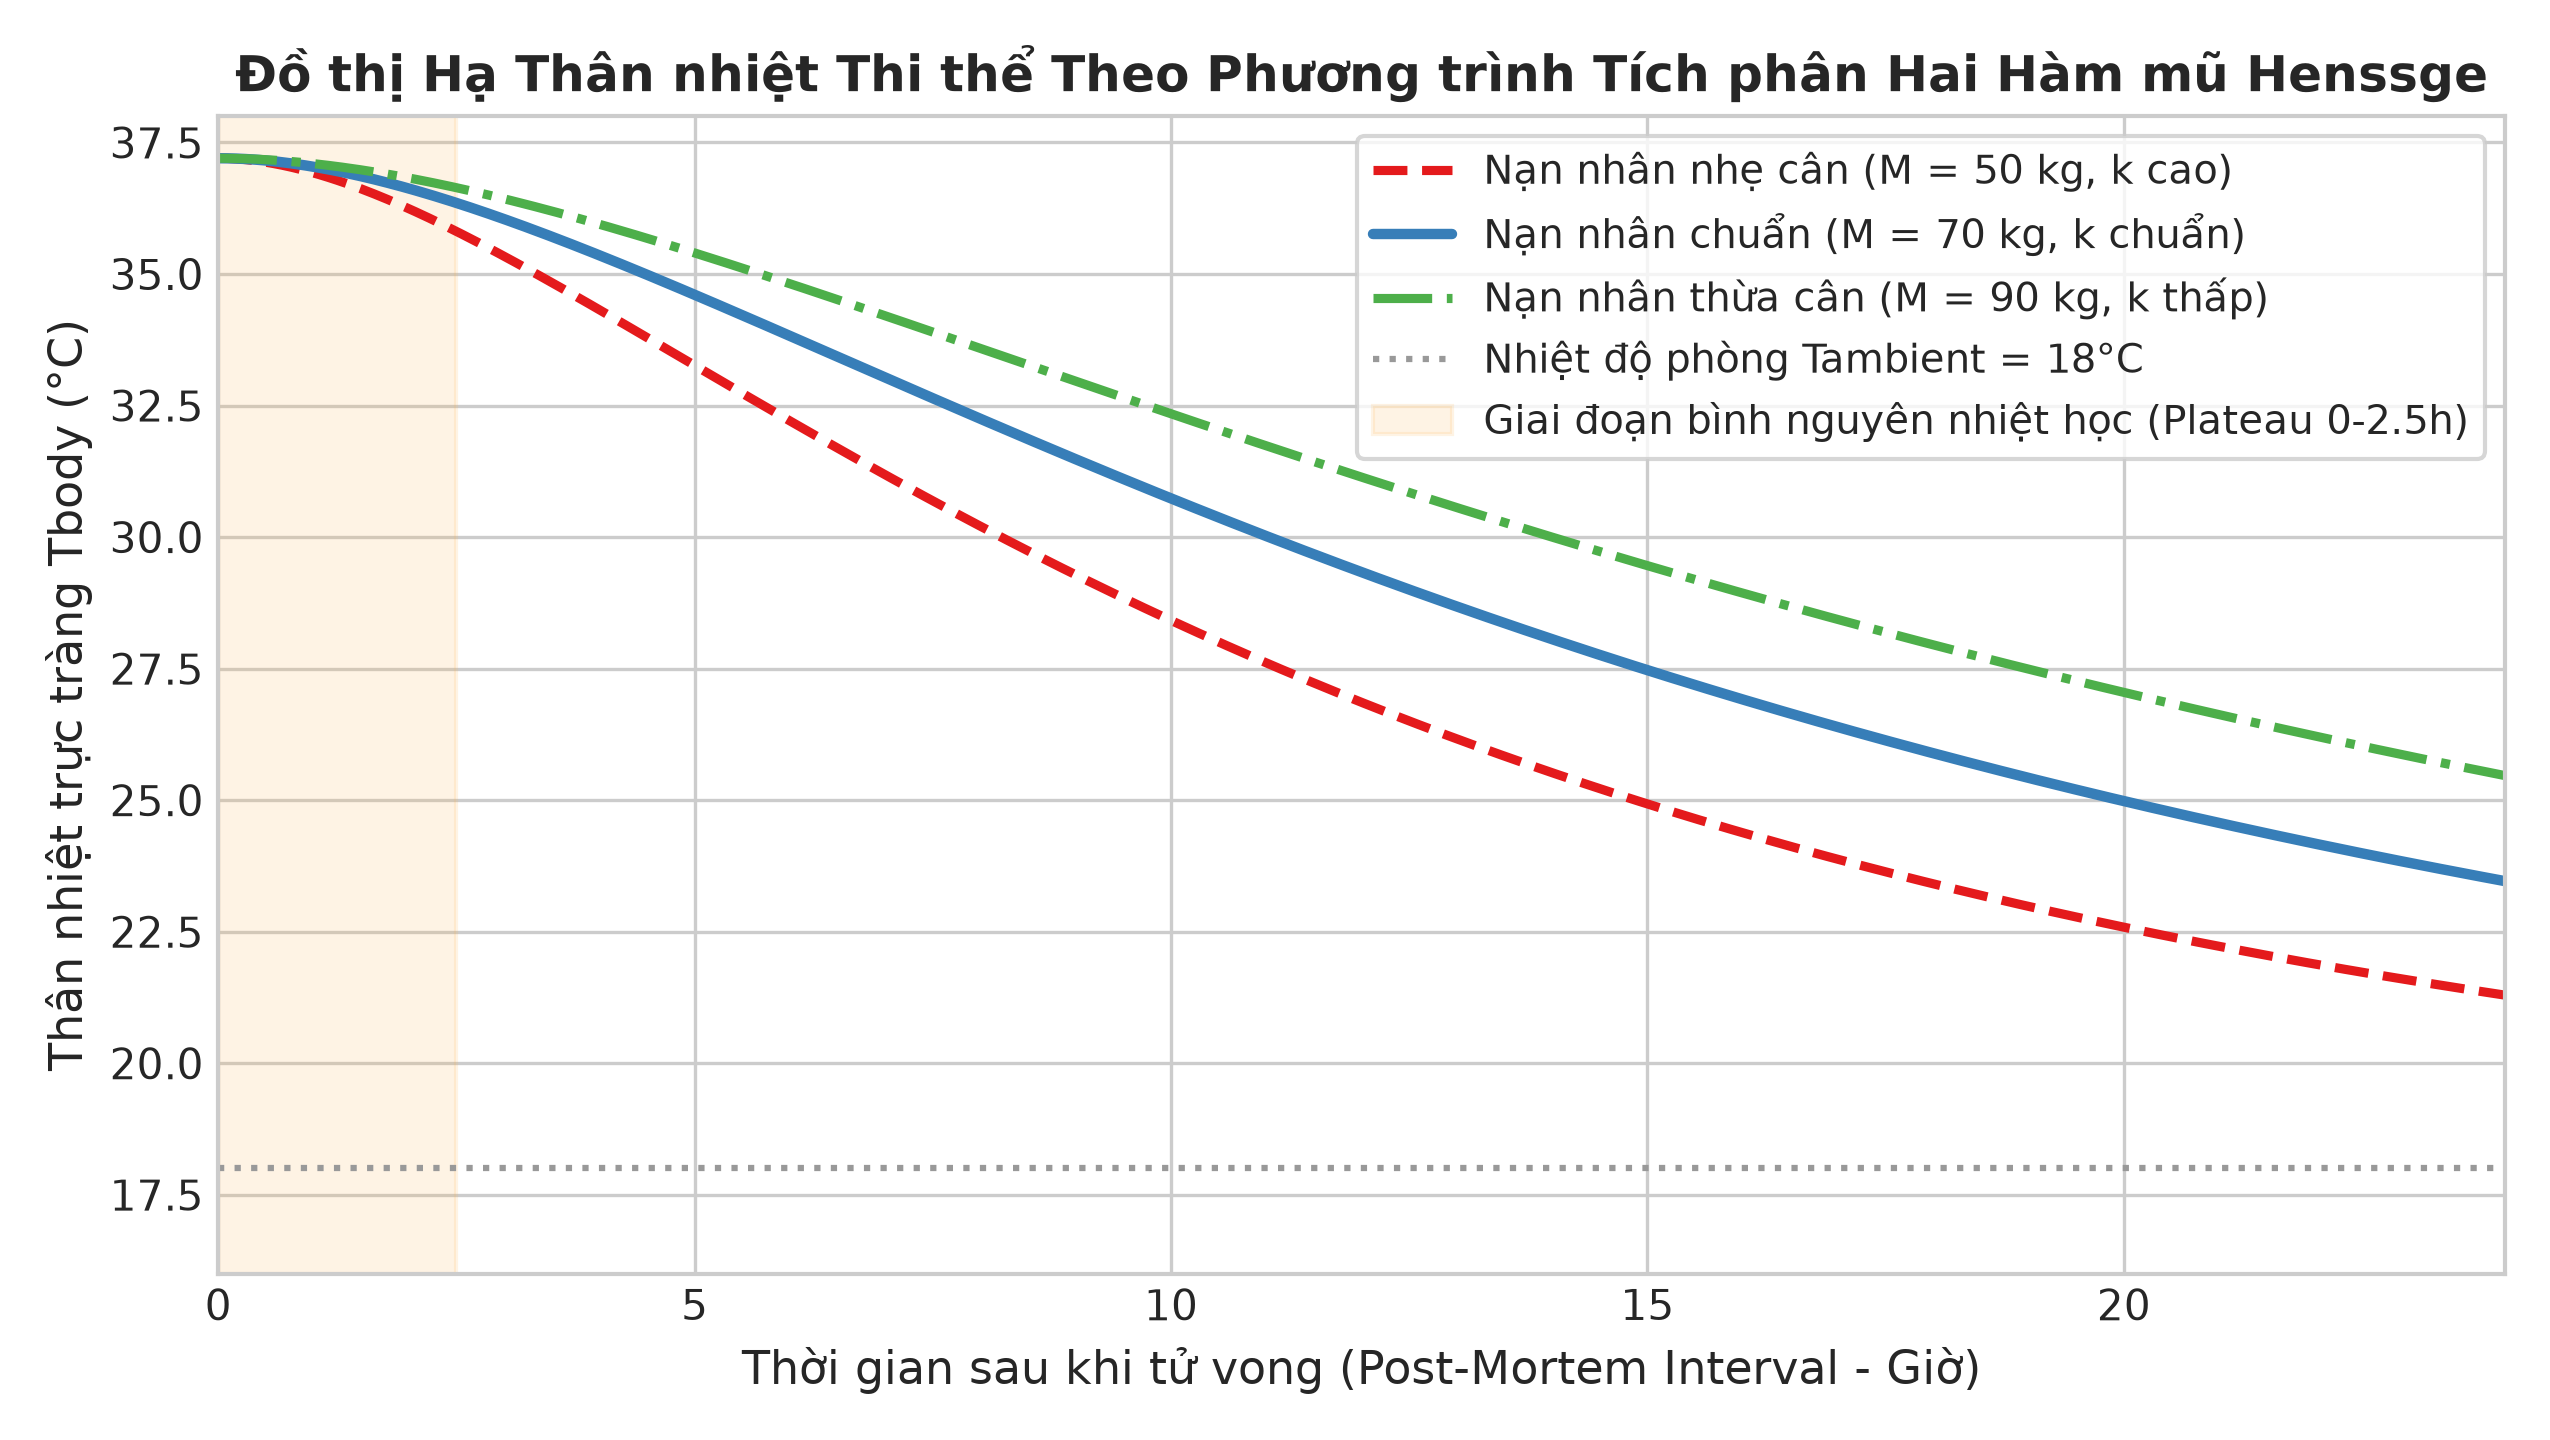
\includegraphics[width=0.85\textwidth]{henssge_curves.png}
    \caption{Đồ thị Hạ thân nhiệt Thi thể Theo Phương trình Hai Hàm mũ Henssge với Các Mức Khối lượng Khác nhau ($T_{\text{ambient}} = 18^\circ\text{C}$)}
    \label{fig:henssge_curves}
\end{figure}

\subsection{Thuật toán Chia đôi Tìm Nghiệm Số và Cửa sổ Tử vong TOD}
Vì phương trình (\ref{eq:henssge_formula}) là phương trình siêu việt đối với $t$ nhưng hàm $\Phi(t)$ đơn điệu giảm ngặt trên $[0, 48]$ giờ từ giá trị $\Phi(0) = 1$, hệ thống sử dụng phương pháp chia đôi (\textit{bisection method}) trên miền $[0, 48]$ giờ với sai số hội tụ $\epsilon = 10^{-4}$ và tối đa $N_{\text{max}} = 100$ bước lặp để tìm nghiệm duy nhất $t^*$ (Thuật toán \ref{alg:henssge_bisection}).

\begin{algorithm}[H]
\caption{Tìm Nghiệm Thời gian Tử vong Henssge Bằng Phương pháp Chia đôi}
\label{alg:henssge_bisection}
\begin{algorithmic}[1]
\Require $T_{\text{body}}$, $T_{\text{ambient}}$, $M$, $C$, Sai số $\epsilon = 10^{-4}$, Số bước tối đa $N_{\text{max}} = 100$
\Ensure Thời gian sau tử vong $t^*$ (giờ) hoặc $\text{None}$ nếu phi vật lý
\State $k \gets \frac{1.2815}{(M \cdot C)^{0.625}} - 0.0284$
\State $\Phi_{\text{target}} \gets \frac{T_{\text{body}} - T_{\text{ambient}}}{37.2 - T_{\text{ambient}}}$
\If{$\Phi_{\text{target}} \le 0$} \Return $\text{None}$ \EndIf
\If{$\Phi_{\text{target}} \ge 1$} \Return $0.0$ \EndIf
\State Định nghĩa $\Phi(t)$ theo (\ref{eq:henssge_formula}) ứng với ngưỡng $T_{\text{ambient}} \le 23.2^\circ\text{C}$ hoặc $> 23.2^\circ\text{C}$
\State $a \gets 0.0, \; b \gets 48.0$ \Comment{Biên tìm kiếm từ 0 đến 48 giờ}
\If{$\Phi(b) - \Phi_{\text{target}} > 0$} \Return $\text{None}$ \EndIf
\For{$n = 1$ \textbf{to} $N_{\text{max}}$}
    \State $m \gets (a + b) / 2$
    \State $f(m) \gets \Phi(m) - \Phi_{\text{target}}$
    \If{$|f(m)| < \epsilon$ \textbf{or} $(b - a) / 2 < \epsilon$}
        \State \Return $m$
    \ElsIf{$(\Phi(a) - \Phi_{\text{target}}) \cdot f(m) < 0$}
        \State $b \gets m$
    \Else
        \State $a \gets m$
    \EndIf
\EndFor
\State \Return $(a + b) / 2$
\end{algorithmic}
\end{algorithm}

Với dung sai tin cậy tiêu chuẩn $\Delta t = \pm 1.5$ giờ từ thời điểm phát hiện thi thể $T_{\text{discovery}}$, cửa sổ thời gian tử vong (TOD) được động cơ ký hiệu tính trực tiếp và gán khóa cứng cho hồ sơ:
\begin{equation}
    TOD = \left[ T_{\text{discovery}} - (t^* + 1.5), \; T_{\text{discovery}} - \max(0, t^* - 1.5) \right]
\end{equation}

Mọi hồ sơ hợp lệ phải thỏa mãn ràng buộc vật lý:
\begin{equation}
    T_{\text{actual\_crime\_time}} \in TOD
\end{equation}

\section{Biểu diễn Đồ thị Hai phía và Ràng buộc Giải được của Vụ án}
\label{sec:theory_graph}

\subsection{Mô hình hóa Vụ án Dưới dạng Đồ thị Hai phía}
Để kiểm tra cấu trúc suy luận giữa lời khai và vật chứng một cách tường minh, hồ sơ vụ án được ánh xạ sang một đồ thị hai phía có hướng:
\begin{equation}
    G = (V_N \cup V_P, E_R)
\end{equation}
Trong đó:
\begin{itemize}[leftmargin=1.5cm]
    \item Phân hoạch thứ nhất $V_N$ biểu diễn tầng tường thuật gồm các đỉnh nghi phạm $V_S = \{s_1, \dots, s_n\}$ và các đỉnh lời khai ngoại phạm tương ứng;
    \item Phân hoạch thứ hai $V_P$ biểu diễn tầng thực tế hiện trường gồm các đỉnh chứng cứ $V_E = \{e_1, \dots, e_m\}$ và mốc sự kiện thời gian gây án;
    \item Tập cạnh $E_R$ biểu diễn các quan hệ ngữ nghĩa đã gán nhãn giữa hai phân hoạch.
\end{itemize}

\begin{figure}[H]
    \centering
    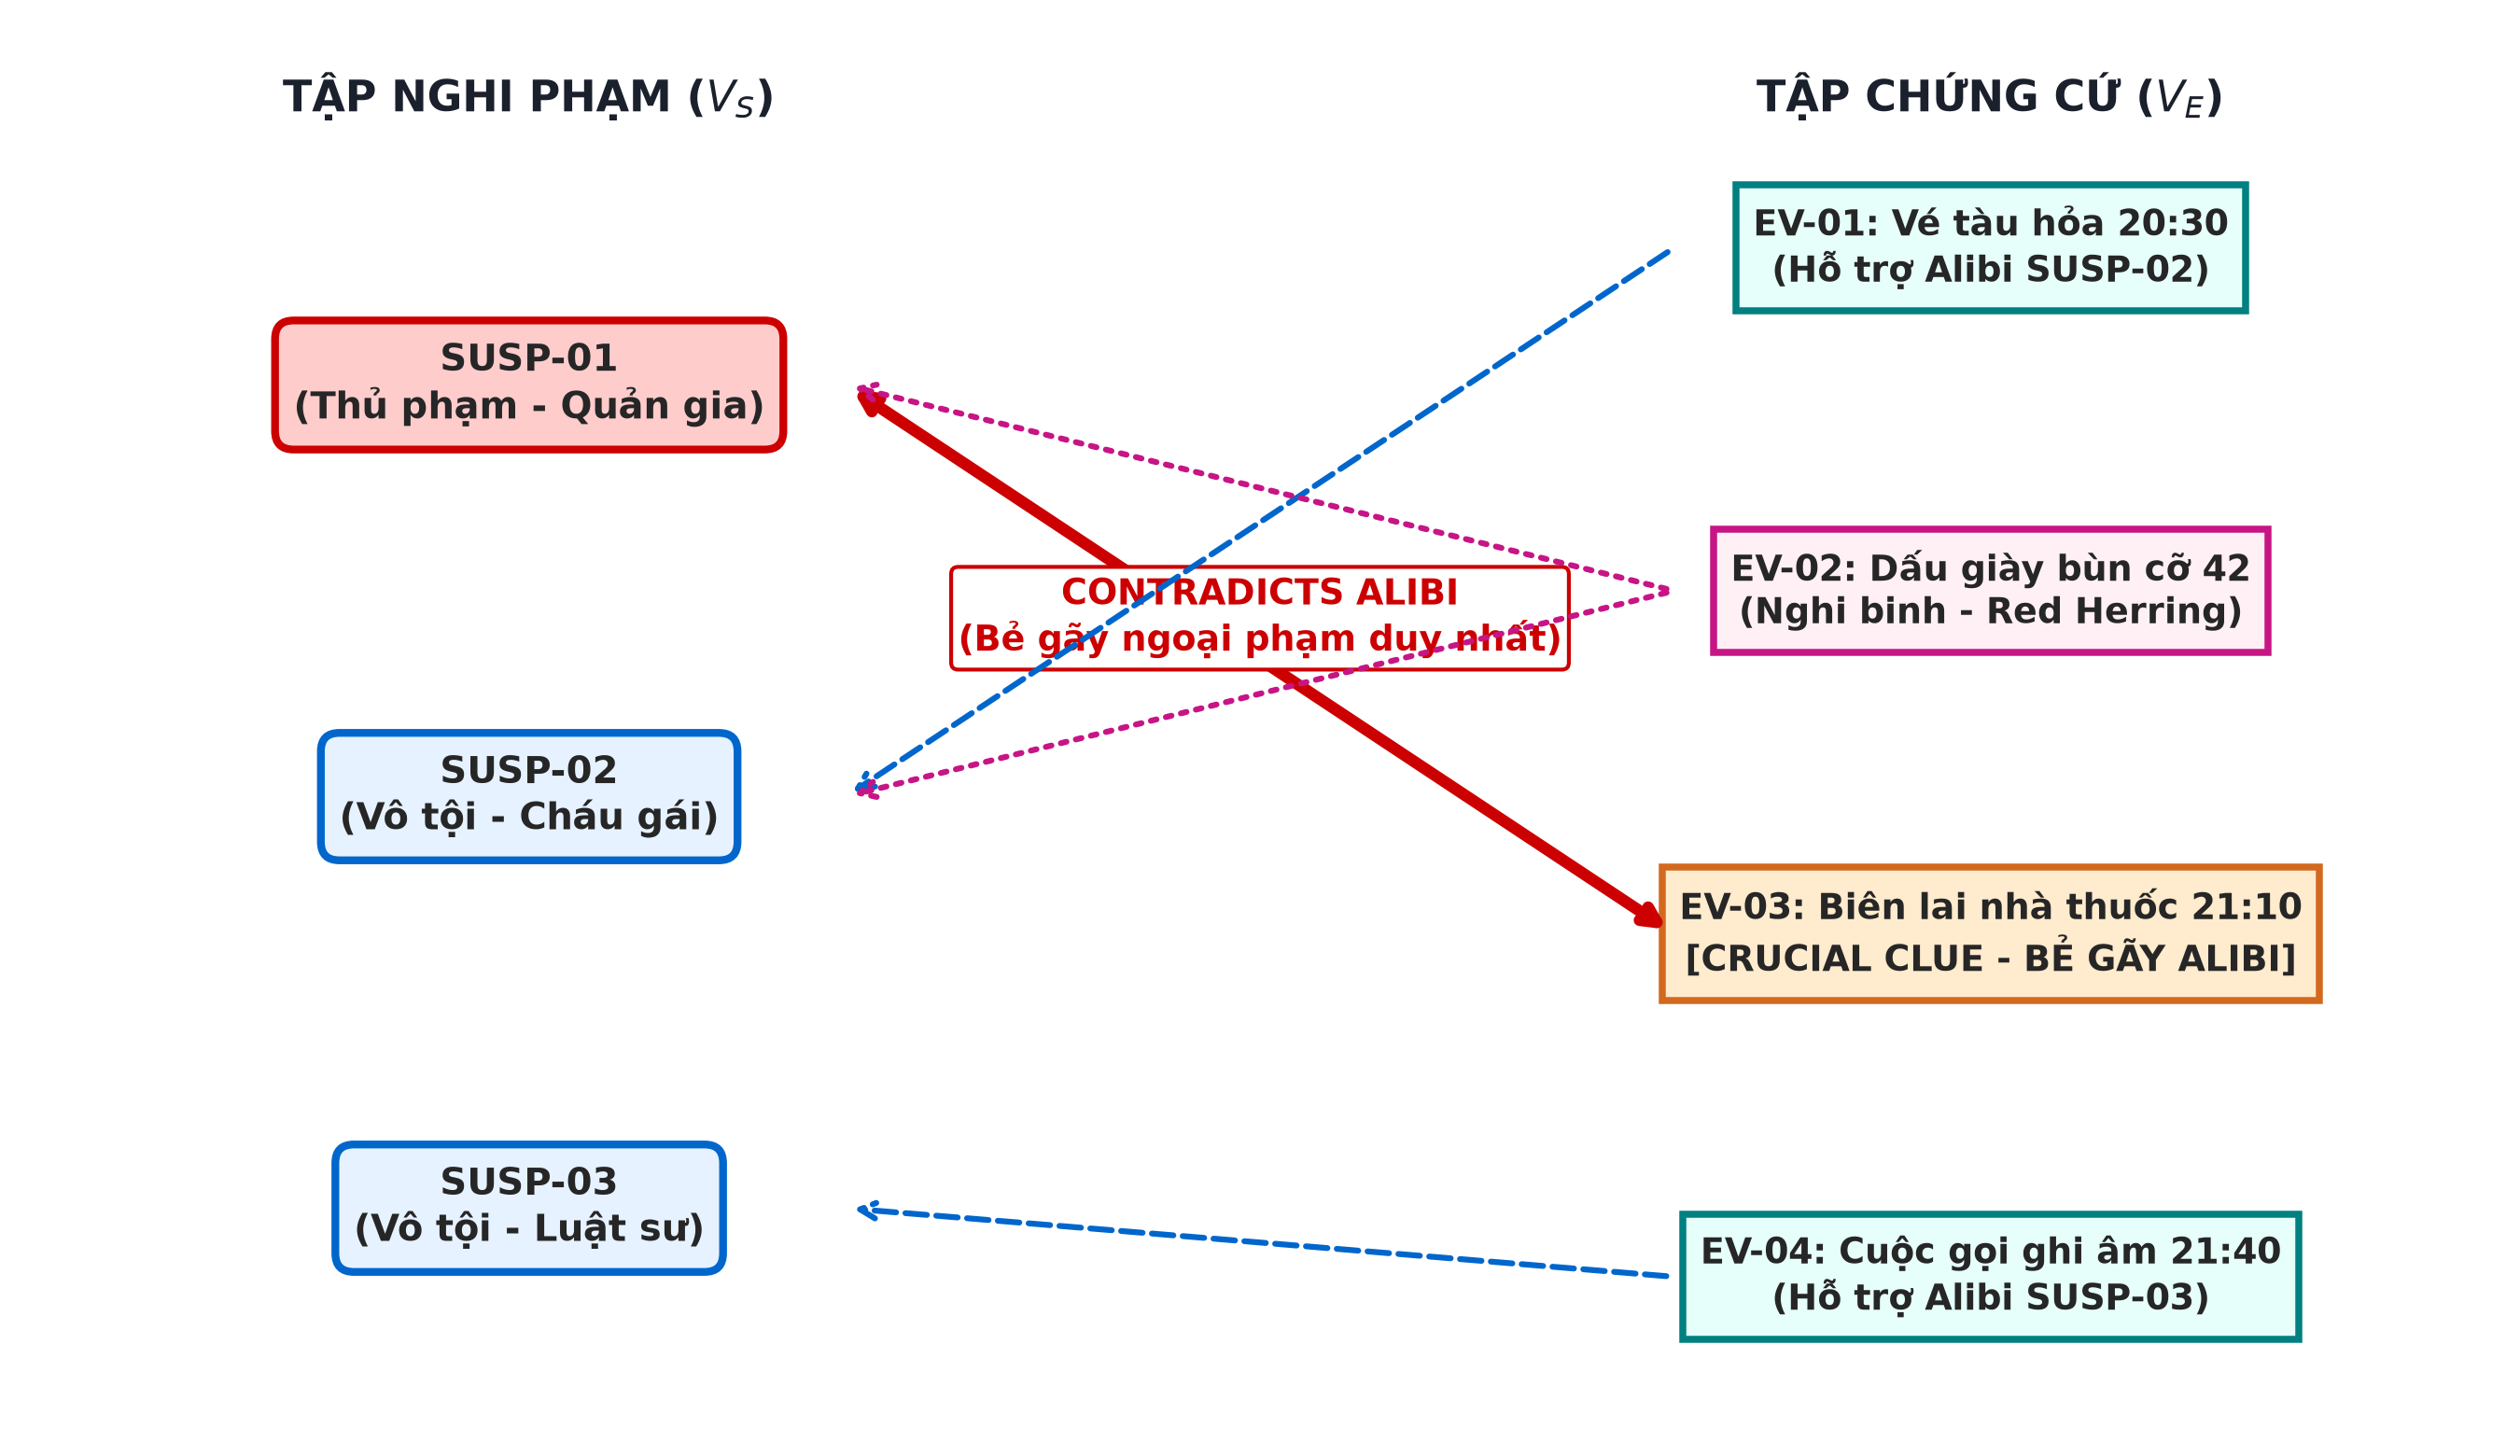
\includegraphics[width=0.90\textwidth]{bipartite_graph.png}
    \caption{Mô hình Đồ thị Hai phía Minh họa Quan hệ Giữa Tập Nghi phạm ($V_S$) và Tập Chứng cứ ($V_E$)}
    \label{fig:bipartite_graph_diagram}
\end{figure}

Các cạnh liên kết trong đồ thị được phân loại thành ba nhóm quan hệ chính:
\begin{enumerate}[leftmargin=1.5cm]
    \item \textbf{Cạnh Tuyên bố / Xác nhận Ngoại phạm:} Liên kết giữa nghi phạm và khung giờ ngoại phạm hoặc chứng cứ hỗ trợ người vô tội.
    \item \textbf{Cạnh Bẻ gãy Ngoại phạm ($E_{\text{contradict}}$):} Liên kết từ vật chứng then chốt (\texttt{is\_crucial = True}) bác bỏ trực tiếp lời khai ngoại phạm của hung thủ.
    \item \textbf{Cạnh manh mối nghi binh (\textit{red herring})} ($E_{\text{herring}}$): Liên kết từ manh mối đánh lạc hướng (\texttt{is\_red\_herring = True}) tới nghi phạm vô tội nhằm giữ độ khó suy luận cho trò chơi.
\end{enumerate}

\subsection{Các Bất biến Thiết kế Bảo đảm Tính Giải được Độc nhất}

\begin{definition}[Khung giờ Ngoại phạm Bao trùm]
Một nghi phạm $s$ có lời khai ngoại phạm che phủ thời điểm phạm tội nếu khoảng thời gian tự khai $[s.\text{alibi\_start}, s.\text{alibi\_end}]$ chứa mốc $T_{\text{actual\_crime\_time}}$ trong cửa sổ $TOD$ (xử lý được cả trường hợp khung giờ vắt qua nửa đêm).
\end{definition}

\begin{invariant}[Hệ Ràng buộc Tính Giải được và Công bằng]
Một hồ sơ vụ án đạt chuẩn kiểm định cấu trúc và giải được công bằng khi tập thực thể và đồ thị $G$ thỏa mãn đồng thời bốn điều kiện tất định sau:
\begin{enumerate}[label=(\roman*)]
    \item \textbf{Tính duy nhất của thủ phạm:} Tồn tại duy nhất một nghi phạm $s^* \in V_S$ được đánh dấu \texttt{is\_culprit = True}, đồng thời định danh của $s^*$ khớp với trường chân lý gốc:
    \begin{equation}
        |\{s \in V_S \mid s.\text{is\_culprit} = \text{True}\}| = 1 \quad \land \quad s^*.\text{id} = \text{GroundTruth.culprit\_id}
    \end{equation}
    
    \item \textbf{Tính tồn tại của chứng cứ phá vỡ ngoại phạm:} Tập vật chứng chứa ít nhất một manh mối then chốt ($\mathcal{C}_{\text{crucial}} = \{e \in V_E \mid e.\text{is\_crucial} = \text{True}\} \neq \emptyset$), bảo đảm nếu thủ phạm có lời khai che phủ thời điểm gây án thì tồn tại đường nối bác bỏ ngoại phạm trên đồ thị.
    
    \item \textbf{Tính toàn vẹn tham chiếu thực thể:} Mọi mã định danh nghi phạm được liên kết bởi các vật chứng hoặc các bước suy luận phải thuộc tập đỉnh hiện hữu $V_S$:
    \begin{equation}
        \forall e \in V_E, \; (e.\text{linked\_suspect\_id} \neq \text{None}) \implies e.\text{linked\_suspect\_id} \in \{s.\text{id} \mid s \in V_S\}
    \end{equation}
    
    \item \textbf{Tính cân bằng yếu tố nghi binh (theo cấu hình sinh án):} Để hạn chế tình huống người chơi đoán đúng chỉ bằng phép loại trừ đơn giản, \texttt{ClueAgent} và bộ kiểm định chất lượng hậu kiểm khuyến nghị bổ sung ít nhất một manh mối đánh lạc hướng gắn với nghi phạm vô tội có bí mật riêng.
\end{enumerate}
\end{invariant}

Trong phần mềm thực tế (\texttt{validator.py} và \texttt{case\_graph.py}), các điều kiện (i), (ii), (iii) cùng ràng buộc nhiệt học Henssge được kiểm tra tất định bằng các phép kiểm tra điều kiện, phép giao tập hợp và duyệt chỉ mục trước khi lưu hồ sơ vào cơ sở dữ liệu.

\section{Hình thức hóa Nguyên tắc Trinh thám Công bằng Knox}
\label{sec:theory_knox}

Bảng \ref{tab:knox_formalization} đối chiếu việc ánh xạ các quy tắc kinh điển trong Mười điều răn của Ronald Knox (1929) \cite{knox1929ten} sang các ràng buộc kỹ thuật được cài đặt trong mã nguồn hệ thống:

\begin{table}[H]
\centering
\caption{Ánh xạ Các Quy tắc Trinh thám Knox sang Ràng buộc Hệ thống}
\label{tab:knox_formalization}
\begin{tabularx}{\textwidth}{p{1.4cm} p{6.2cm} X}
\toprule
\textbf{Điều} & \textbf{Quy tắc Văn học Knox (1929)} & \textbf{Ràng buộc Hệ thống Tương ứng} \\
\midrule
\textbf{Điều 1} & Không có yếu tố siêu nhiên hay ma quái can thiệp vào vụ án. & Thời điểm tử vong và hạ thân nhiệt phải thỏa mãn phương trình nhiệt học Henssge. \\
\textbf{Điều 2} & Không dùng các chất độc giả tưởng chưa được khoa học biết đến. & Vũ khí và nguyên nhân tử vong phải là vật thể hoặc cơ chế vật lý có thật. \\
\textbf{Điều 3} & Không giấu lối đi bí mật chưa từng được mô tả trước. & Toàn bộ địa điểm hiện trường và vị trí thu giữ vật chứng được công bố trong hồ sơ. \\
\textbf{Điều 4} & Thủ phạm phải xuất hiện từ đầu, không thêm nhân vật lúc kết thúc. & Toàn bộ nghi phạm cố định trong $V_S$; ràng buộc \texttt{culprit\_id} phải thuộc tập $\{s.\text{id}\}$. \\
\textbf{Điều 5} & Thám tử điều tra không được tự mình là hung thủ. & Vai trò người chơi tách biệt hoàn toàn với danh sách nghi phạm $V_S$. \\
\textbf{Điều 6} & Không phá án nhờ trực giác hay trùng hợp ngẫu nhiên. & Hàm chấm điểm yêu cầu chọn đúng $s^*$ đồng thời nộp ít nhất một vật chứng thuộc $\mathcal{C}_{\text{crucial}}$. \\
\textbf{Điều 7} & Không dùng anh chị em sinh đôi chưa báo trước làm ngoại phạm giả. & Kiểm tra trùng lặp mã định danh trên toàn bộ tập nghi phạm và vật chứng. \\
\textbf{Điều 8} & Không giấu giếm người chơi các manh mối quan trọng. & Toàn bộ các vật chứng trong $V_E$ đều được truyền và hiển thị trên bảng điều tra. \\
\bottomrule
\end{tabularx}
\end{table}

\section{Khảo cứu và Phân tích Đối chiếu Các Công trình Liên quan}
\label{sec:theory_related_works}

Việc ứng dụng AI vào đánh giá suy luận và tạo sinh tự sự trinh thám đã nhận được sự quan tâm rộng rãi từ cộng đồng xử lý ngôn ngữ tự nhiên. Dưới đây là phân tích đối chiếu ba công trình tiêu biểu công bố trên các hội nghị khoa học uy tín:

\subsection{Bộ đánh giá Suy luận MuSR (Sprague và cộng sự, ICLR 2024)}
Công trình \textit{MuSR} của nhóm nghiên cứu Đại học Texas tại Austin \cite{sprague2024musr} xây dựng bộ dữ liệu đánh giá khả năng suy luận nhiều bước trên văn bản tự sự tự nhiên, trong đó trọng tâm là tập kịch bản án mạng bí ẩn dài khoảng 1,000 từ. MuSR áp dụng quy trình tổng hợp neuro-symbolic từ cây suy luận sang văn bản nhằm tạo bài toán kiểm tra năng lực CoT của GPT-4 và các mô hình tương đương. Kết quả cho thấy ngay cả các mô hình mạnh vẫn gặp sai sót khi theo dõi nhiều mối quan hệ phụ thuộc dài. Tuy nhiên, MuSR được thiết kế như một \textbf{bộ benchmark đánh giá thụ động}, không phải một hệ thống trò chơi tương tác thời gian thực, không tích hợp mô hình nhiệt học y pháp Henssge và không hỗ trợ cơ chế vá lỗi cục bộ theo phản hồi kiểm định.

\subsection{Khung Đa tác tử Deciphering Digital Detectives (Wu và cộng sự, ACL 2024)}
Công trình \textit{Deciphering Digital Detectives} \cite{wu2024deciphering} nghiên cứu hành vi của các tác tử LLM khi tham gia trò chơi nhập vai trinh thám kịch bản \textit{Jubensha} (dạng kịch bản án mạng nhiều người chơi phổ biến). Các tác giả xây dựng bộ dữ liệu từ kịch bản có sẵn và tổ chức hệ đa tác tử đóng vai nghi phạm, trao đổi thông tin, che giấu động cơ và suy luận tìm hung thủ dưới sự hỗ trợ của máy trạng thái hữu hạn (FSM) hoặc prompt điều phối. Dù làm rõ được hành vi tương tác xã hội của LLM, công trình này tập trung vào việc cho tác tử \textit{chơi trên kịch bản đã soạn sẵn bởi con người}, chưa giải quyết bài toán tự động tạo sinh vụ án mới có kiểm chứng tính giải được bằng đồ thị và ràng buộc vật lý.

\subsection{Hệ thống Phát hiện Tự mâu thuẫn ContraDoc (Li và cộng sự, NAACL 2024)}
Công trình \textit{ContraDoc} \cite{li2024contradoc} đề xuất tập dữ liệu gán nhãn thủ công nhằm đo lường khả năng phát hiện các mâu thuẫn tự thân bên trong văn bản dài của các LLM. Nghiên cứu chứng minh LLM dễ bỏ sót các xung đột logic ngầm định nằm cách xa nhau theo dòng thời gian hoặc trạng thái sự kiện. Tương tự MuSR, ContraDoc đóng vai trò là bài toán \textbf{phân loại và phát hiện lỗi hậu kiểm trên văn bản tổng quát}, chưa tích hợp vào vòng lặp sinh kịch bản trò chơi có kiến trúc sửa lỗi cục bộ và chấm điểm suy luận người chơi.

\subsection{Bảng Tổng hợp Đối sánh}
Bảng \ref{tab:related_works_comparison} tóm tắt điểm khác biệt giữa hệ thống do tác giả đề xuất và ba công trình liên quan nêu trên:

\begin{table}[H]
\centering
\caption{Đối sánh Giữa Hệ thống Đề xuất và Các Công trình Nghiên cứu Liên quan}
\label{tab:related_works_comparison}
\begin{tabularx}{\textwidth}{l X X X}
\toprule
\textbf{Tiêu chí So sánh} & \textbf{MuSR (ICLR 2024)} & \textbf{Digital Detectives (ACL 2024)} & \textbf{Hệ thống Đề xuất} \\
\midrule
\textbf{Mục tiêu chính} & Đánh giá suy luận nhiều bước của LLM & Thử nghiệm tác tử chơi kịch bản có sẵn & Sinh vụ án mới và xác thực trò chơi tương tác \\
\textbf{Kiến trúc xử lý} & Sinh cây logic sang văn bản tĩnh & Đa tác tử nhập vai theo kịch bản & Chuỗi 4 tác tử kết hợp bộ kiểm định tất định \\
\textbf{Ràng buộc y pháp} & Không áp dụng & Không áp dụng & \textbf{Phương trình Henssge + Bisection} \\
\textbf{Kiểm định tính giải được} & Sinh từ cây suy luận tĩnh trước & Kịch bản biên soạn thủ công & \textbf{Đồ thị hai phía + Kiểm định 7 mã lỗi} \\
\textbf{Cơ chế xử lý lỗi} & Không có sửa lỗi tự động & Không có cơ chế vá cấu trúc & \textbf{Sửa lỗi cục bộ ($\mathcal{O}(1)$ ngữ cảnh)} \\
\textbf{Chấm điểm người chơi} & So khớp trắc nghiệm tĩnh & Tác tử tự đánh giá & \textbf{Tất định trong bộ nhớ ($< 0.1\text{ms}$)} \\
\textbf{Giao diện ứng dụng} & Tập dữ liệu nghiên cứu & Môi trường mô phỏng dòng lệnh & \textbf{Unity 6 URP 2D (Phòng Co-op LAN)} \\
\bottomrule
\end{tabularx}
\end{table}

\chapter{PHÂN TÍCH VÀ THIẾT KẾ KIẾN TRÚC HỆ THỐNG}
\label{ch:architecture}

\section{Các Quyết định Kiến trúc Cốt lõi}
\label{sec:arch_adrs}

Một hệ thống phần mềm AI hoàn chỉnh không chỉ được đánh giá qua độ phức tạp thuật toán, mà còn thông qua việc cân nhắc thấu đáo các đánh đổi kỹ thuật ở từng tầng thiết kế. Trong quá trình phát triển đồ án, tác giả đã thiết lập 7 bản ghi quyết định kiến trúc (ADR\textsuperscript{2}) làm cơ sở lựa chọn công nghệ và đối sánh trực diện với các lựa chọn thay thế như tổng hợp tại Bảng \ref{tab:framework_comparison}:

\subsection{ADR-001: Lựa chọn Ngôn ngữ Python và Web Framework FastAPI}
\begin{itemize}[leftmargin=1.5cm]
    \item \textbf{Đặt vấn đề:} Máy chủ backend phải đáp ứng đồng thời hai dạng tải trái ngược nhau: (i) giữ kết nối mạng chờ chuỗi 4 tác tử LLM sinh kịch bản tuần tự kéo dài 10--20 giây (tác vụ chờ vào/ra mạng cao), và (ii) duy trì kênh đồng bộ phòng chơi nhóm tối đa 3 thám tử qua WebSocket (\texttt{rooms.py}) song song với các phép tính số học nội tại (giải phương trình Henssge, duyệt đồ thị kiểm chứng, chấm điểm kết án) có độ trễ dưới 5 mili-giây.
    \item \textbf{Các phương án cân nhắc:}
    \begin{enumerate}
        \item \textit{Django (Python):} Đầy đủ tính năng quản trị và kết xuất trang phía máy chủ, nhưng kiến trúc nguyên khối mang theo nhiều thành phần dư thừa đối với dịch vụ định tuyến API thuần JSON và chi phí chuyển ngữ cảnh bất đồng bộ cao.
        \item \textit{Flask (Python):} Gọn nhẹ nhưng mặc định vận hành theo chuẩn giao diện cổng máy chủ đồng bộ (WSGI), làm khóa cứng luồng xử lý của máy chủ trong suốt 10--20 giây chờ phản hồi từ LLM nếu không cấu hình máy chủ phụ trợ phức tạp, đồng thời thiếu cơ chế kiểm chuẩn lược đồ dữ liệu tự động tích hợp sẵn ở tầng định tuyến.
        \item \textit{Node.js (TypeScript):} Xử lý vào/ra bất đồng bộ tốt, nhưng không tương thích trực tiếp với hệ sinh thái tính toán khoa học, phân tích thực nghiệm (\texttt{pandas}, \texttt{matplotlib}) và các thư viện AI bằng Python của phần lõi backend.
        \item \textit{FastAPI (Python 3.13):} Framework hiệu năng cao xây dựng trên chuẩn giao diện máy chủ bất đồng bộ và Pydantic \cite{fastapi2024}.
    \end{enumerate}
    \item \textbf{Quyết định Kiến trúc:} Lựa chọn \textbf{FastAPI trên nền Python 3.13} (phiên bản cài đặt thực tế FastAPI 0.137.1 trên máy chủ Uvicorn 0.49.0).
    \item \textbf{Lý do lựa chọn:} Vòng lặp sự kiện bất đồng bộ nguyên bản (\texttt{async/await}) cho phép máy chủ xử lý nhiều phiên sinh kịch bản và kết nối WebSocket cùng lúc mà không làm nghẽn tiến trình khi chờ LLM; tích hợp trực tiếp Pydantic v2 ngay tại tầng định tuyến HTTP để tự động từ chối gói tin sai cấu trúc; và tự động sinh tài liệu đặc tả OpenAPI tại \texttt{/docs} phục vụ đồng bộ hợp đồng dữ liệu với Unity Client.
\end{itemize}

\subsection{ADR-002: Lựa chọn Thư viện Kiểm chuẩn Dữ liệu Pydantic v2}
\begin{itemize}[leftmargin=1.5cm]
    \item \textbf{Đặt vấn đề:} Đầu ra từ LLM có thể gặp lỗi cú pháp định dạng JSON, thiếu trường bắt buộc, sai định dạng giờ 24 giờ hoặc vượt ngưỡng sinh học hợp lý. Hệ thống cần một tầng kiểm chuẩn lược đồ nghiêm ngặt ngay tại cổng tiếp nhận.
    \item \textbf{Các phương án cân nhắc:}
    \begin{enumerate}
        \item \textit{Thư viện chuẩn \texttt{dataclasses} (Python):} Chỉ định nghĩa cấu trúc lưu trữ thuộc tính, không hỗ trợ tự động ép kiểu hay kiểm tra ràng buộc miền giá trị khi giải mã chuỗi JSON thô từ LLM.
        \item \textit{Marshmallow:} Hỗ trợ kiểm chuẩn lược đồ nhưng thực thi hoàn toàn trên trình thông dịch Python nên tốc độ phân giải chậm hơn đáng kể và buộc lập trình viên phải khai báo tách rời lớp mô hình dữ liệu với lớp lược đồ xác thực.
        \item \textit{Pydantic v2} (phiên bản cài đặt thực tế 2.14.3) \cite{pydantic2024}.
    \end{enumerate}
    \item \textbf{Quyết định Kiến trúc:} Lựa chọn \textbf{Pydantic v2} làm hợp đồng dữ liệu xuyên suốt từ tầng gọi tác tử LLM đến tầng giao tiếp API.
    \item \textbf{Lý do lựa chọn:} Lõi xác thực \texttt{pydantic-core} biên dịch bằng ngôn ngữ Rust mang lại tốc độ phân giải JSON nhanh hơn rõ rệt so với kiểm tra thuần Python; cho phép khai báo ràng buộc miền giá trị trực tiếp trên thuộc tính (như \texttt{Field(ge=30.0, le=200.0)} cho cân nặng và \texttt{Field(ge=0.3, le=2.0)} cho hệ số làm lạnh), kiểm định chuẩn hóa giờ \texttt{HH:MM} qua \texttt{@field\_validator}, cũng như đối sánh biểu thức chính quy (như kiểm tra định dạng giờ \texttt{\textasciicircum(\textbackslash d\{1,2\}):(\textbackslash d\{2\})(?::\textbackslash d\{2\})?\textdollar} hay quy ước mã thực thể \texttt{\textasciicircum SUSP-\textbackslash d\{2\}\textdollar}) để ngắt sớm các dữ liệu hỏng cú pháp trước khi đi vào bộ kiểm định ký hiệu.
\end{itemize}

\subsection{ADR-003: Thiết kế Kiến trúc Dịch vụ Web Kết hợp Client Unity 6 URP 2D Đa nền tảng}
\begin{itemize}[leftmargin=1.5cm]
    \item \textbf{Đặt vấn đề:} Ở giai đoạn thử nghiệm ban đầu, tôi đã xây dựng nguyên mẫu giao diện Web bằng React (\texttt{V0/frontend/}). Tuy nhiên, khi chuyển sang hoàn thiện trải nghiệm bàn làm việc thám tử với ánh sáng động, nhiều lớp thẻ ảnh kéo thả, dây chỉ đỏ co giãn và tính năng tìm phòng chơi mạng cục bộ LAN không cần nhập địa chỉ IP thủ công, nguyên mẫu thuần trình duyệt bộc lộ nhiều giới hạn kỹ thuật.
    \item \textbf{Các phương án cân nhắc:}
    \begin{enumerate}
        \item \textit{Thuần Web React:} Dễ truy cập qua trình duyệt nhưng tốn chi phí đồng bộ thao tác kéo thả kết hợp vẽ dây chỉ đỏ trên cây mô hình tài liệu trình duyệt, và bị cơ chế hộp cát bảo mật của trình duyệt (\textit{browser sandbox}) chặn quyền phát gói tin quảng bá UDP ở tầng mạng cục bộ (cổng \texttt{47777} trong \texttt{lan\_discovery.py} và \texttt{LanDiscoveryClient.cs}).
        \item \textit{Unreal Engine 5:} Tối ưu cho đồ họa 3D quy mô lớn nhưng dung lượng bộ cài nặng nề và dư thừa tài nguyên đối với bài toán giao diện bảng ghim 2D/2.5D.
        \item \textit{Godot Engine:} Nhẹ và mã nguồn mở, nhưng hệ thống xử lý hậu kỳ ánh sáng 2D và quy trình đóng gói đồng thời hai đích WebGL và máy trạm chưa thuận tiện bằng hệ sinh thái Unity trong khung thời gian đồ án.
        \item \textit{Kiến trúc Web API kết hợp Unity 6} (bản hỗ trợ dài hạn 6000.5.8f1) trên đường ống kết xuất phổ quát (URP) 2D \cite{unity2024urp}.
    \end{enumerate}
    \item \textbf{Quyết định Kiến trúc:} Tách hệ thống theo mô hình \textbf{Dịch vụ Web phân tán} (\texttt{FastAPI} RESTful API, giao thức HTTP/JSON, WebSockets, cấu hình CORS mở rộng) kết hợp Client \textbf{Unity 6 URP 2D} hỗ trợ xuất bản đa nền tảng (mục tiêu trình duyệt WebGL và tệp thực thi độc lập).
    \item \textbf{Lý do lựa chọn:} Giải pháp này vừa duy trì trọn vẹn kiến trúc dịch vụ Web và khả năng xuất bản WebGL trên trình duyệt, vừa cho phép dựng giao diện gắn với không gian bàn điều tra (\texttt{BankersLampController.cs} điều khiển độ sáng bóng sợi đốt, \texttt{CorkboardManager.cs} kéo thả ảnh Polaroid kèm dây chỉ đỏ động thời gian thực), khóa tỉ lệ hiển thị chuẩn $1920\times 1080$ (16:9) và mở khóa socket UDP phục vụ tự động tìm phòng chơi LAN tại cổng \texttt{47777}.
\end{itemize}

\subsection{ADR-004: Lựa chọn Đường ống Đa tác tử Tự chủ thay vì Prompt Nguyên khối hay Khung Trừu tượng Nặng}
\begin{itemize}[leftmargin=1.5cm]
    \item \textbf{Đặt vấn đề:} Biên soạn một vụ án trinh thám hoàn chỉnh đòi hỏi đồng thời cốt truyện, thông số pháp y, lời khai từng nghi phạm, chứng cứ bẻ gãy ngoại phạm và chuỗi lập luận giải đố.
    \item \textbf{Các phương án cân nhắc:} (1) Gọi một câu lệnh nguyên khối duy nhất; (2) Sử dụng các khung điều phối đa tác tử cỡ lớn như \texttt{LangChain} hoặc \texttt{AutoGen} vốn chèn nhiều lớp bọc trung gian làm khó kiểm soát chuỗi chỉ dẫn nguyên bản và phát sinh độ trễ phụ trội; (3) Tự cài đặt đường ống gọn nhẹ kế thừa trực tiếp \texttt{AsyncOpenAI}.
    \item \textbf{Quyết định Kiến trúc:} Phân rã quá trình sinh thành \textbf{4 tác tử chuyên biệt chạy tuần tự}: \texttt{OutlineAgent} $\to$ \texttt{CharacterAgent} $\to$ \texttt{ClueAgent} $\to$ \texttt{DeductionAgent}, cài đặt trực tiếp trên lớp nền \texttt{BaseAgent} trong \texttt{agents.py}.
    \item \textbf{Lý do lựa chọn:} Chia nhỏ gánh nặng suy luận cho LLM theo từng lược đồ JSON hẹp giúp tỷ lệ hợp lệ cú pháp đạt 100\% trong thực nghiệm; tách biệt khâu thiết lập chân lý gốc ở \texttt{OutlineAgent} với khâu tạo lời khai và manh mối ở các tác tử sau; đồng thời cho phép gắn cơ chế tự động chuyển mạch dự phòng ở từng tác tử (\texttt{FALLBACK\_CANDIDATES}) khi mô hình chính gặp lỗi hạn mức hoặc gián đoạn mạng.
\end{itemize}

\subsection{ADR-005: Lựa chọn Cơ chế Sửa lỗi Cục bộ}
\begin{itemize}[leftmargin=1.5cm]
    \item \textbf{Quyết định Kiến trúc:} Thay vì hủy toàn bộ hồ sơ và sinh lại từ đầu khi có lỗi logic, bộ điều phối áp dụng cơ chế sửa lỗi cục bộ có định hướng theo trường \texttt{component} (\texttt{outline}, \texttt{character}, \texttt{clue}) của \texttt{ConstraintViolation}.
    \item \textbf{Lý do lựa chọn:} Chỉ tái xử lý thành phần phát sinh lỗi với ngữ cảnh thu gọn hằng số $\mathcal{O}(1)$, hạn chế chi phí token và thời gian khôi phục so với tái sinh toàn bộ đường ống $\mathcal{O}(N)$.
\end{itemize}

\subsection{ADR-006: Điều phối Mô hình qua Cổng Proxy Gateway Cục bộ}
\begin{itemize}[leftmargin=1.5cm]
    \item \textbf{Đặt vấn đề:} Thực nghiệm đối sánh đòi hỏi gọi nhiều dòng mô hình khác nhau (OpenAI GPT, Google Gemini/Gemma, mô hình cục bộ Ollama) qua cùng một giao diện lập trình thống nhất, xử lý giới hạn tốc độ và tách biệt khóa xác thực thay vì duy trì nhiều bộ công cụ phát triển riêng lẻ cho từng nhà cung cấp.
    \item \textbf{Quyết định Kiến trúc:} Kết nối qua cổng Proxy Gateway cục bộ (\texttt{9Router}) tại địa chỉ \texttt{http://localhost:20128/v1}, tương thích chuẩn giao thức OpenAI.
    \item \textbf{Lý do lựa chọn:} Cho phép chuyển đổi mô hình linh hoạt ở thời điểm chạy qua API \texttt{POST /api/settings} hoặc chuyển hướng dự phòng sang máy chủ Ollama nội bộ (\texttt{http://localhost:11434/v1}) mà không cần chỉnh sửa mã nguồn các tác tử, đồng thời hỗ trợ ghi nhận thời gian phản hồi thực tế phục vụ đánh giá thực nghiệm.
\end{itemize}

\subsection{ADR-007: Lựa chọn Cơ sở dữ liệu Quan hệ Nhúng SQLite (Chế độ WAL) và SQLAlchemy 2.0}
\begin{itemize}[leftmargin=1.5cm]
    \item \textbf{Đặt vấn đề:} Hệ thống cần lưu trữ bền vững hồ sơ vụ án, lịch sử kết án của người chơi và nhật ký thực nghiệm benchmark, bảo đảm tính toàn vẹn tham chiếu giữa vụ án và các lượt phá án nhưng không làm phức tạp hóa quá trình đóng gói khi phân phối trò chơi tới người dùng cuối.
    \item \textbf{Các phương án cân nhắc:}
    \begin{enumerate}
        \item \textit{Lưu tệp JSON rời thuần túy:} Dễ gặp rủi ro hỏng tệp khi nhiều luồng ghi đồng thời và không hỗ trợ truy vấn thống kê độ khó theo thời gian thực.
        \item \textit{Hệ quản trị khách--chủ PostgreSQL hoặc MySQL:} Mạnh mẽ cho hệ thống lớn nhiều máy chủ, nhưng đòi hỏi người dùng phải cài đặt dịch vụ cơ sở dữ liệu nền hoặc Docker, không phù hợp với mục tiêu triển khai gọn nhẹ kèm gói trò chơi thực thi độc lập.
        \item \textit{Cơ sở dữ liệu phi quan hệ MongoDB:} Lưu tài liệu JSON tự nhiên nhưng thiếu cơ chế ràng buộc khóa ngoại cưỡng bức và xóa dây chuyền ở tầng lưu trữ giữa hồ sơ vụ án với lịch sử kết án.
        \item \textit{SQLite chế độ WAL kết hợp SQLAlchemy 2.0} (phiên bản cài đặt 2.0.51).
    \end{enumerate}
    \item \textbf{Quyết định Kiến trúc:} Sử dụng \textbf{SQLite} bật cơ chế ghi nhật ký trước (WAL\textsuperscript{23}) làm tầng lưu trữ quan hệ nhúng thông qua thư viện ánh xạ đối tượng -- quan hệ \textbf{SQLAlchemy 2.0}.
    \item \textbf{Lý do lựa chọn:} Chỉ thị \texttt{PRAGMA journal\_mode=WAL} cho phép nhiều luồng đọc đồng thời không bị khóa bởi thao tác ghi trong chế độ phối hợp nhóm 3 người chơi; \texttt{PRAGMA foreign\_keys=ON} bảo đảm tính toàn vẹn tham chiếu \texttt{ON DELETE CASCADE} giữa bảng \texttt{cases} và \texttt{deduction\_logs} đạt chuẩn ACID; đồng thời toàn bộ cơ sở dữ liệu gói gọn trong một tệp đơn lẻ không cần cài đặt máy chủ phụ trợ.
\end{itemize}

\begin{table}[H]
\centering
\caption{Đối sánh Tổng hợp Lựa chọn Công nghệ và Framework Theo Từng Tầng Hệ thống}
\label{tab:framework_comparison}
\begin{tabularx}{\textwidth}{p{2.6cm} p{3.0cm} p{4.0cm} X}
\toprule
\textbf{Tầng Kiến trúc} & \textbf{Công nghệ Chọn} & \textbf{Phương án Đối chứng} & \textbf{Ưu thế Kỹ thuật Quyết định} \\
\midrule
\textbf{Web API \& Điều phối} & FastAPI 0.137.1 (ASGI / Uvicorn) & Flask (WSGI), Django, Node.js & Xử lý bất đồng bộ không khóa luồng khi chờ LLM 10--20s; hỗ trợ WebSocket phòng chơi nhóm và đồng bộ OpenAPI với Python AI. \\
\textbf{Kiểm chuẩn Lược đồ} & Pydantic v2.14.3 (Rust core) & Python \texttt{dataclasses}, Marshmallow & Tốc độ phân giải nhanh nhờ nhân Rust; ép kiểu và bắt lỗi biểu thức chính quy trực tiếp tại biên giới API. \\
\textbf{Điều phối Đa tác tử} & \texttt{BaseAgent} thuần trên \texttt{AsyncOpenAI} & Prompt nguyên khối, LangChain / AutoGen & Kiểm soát trực tiếp prompt và lược đồ JSON hẹp; giảm lớp bọc trung gian; hỗ trợ chuyển mạch dự phòng theo từng tác tử. \\
\textbf{Lưu trữ Dữ liệu} & SQLite (WAL) + SQLAlchemy 2.0.51 & Tệp JSON rời, PostgreSQL, MongoDB & Đạt chuẩn ACID và khóa ngoại \texttt{CASCADE}; đọc/ghi song song không nghẽn nhờ WAL; nhúng gọn không cần cài máy chủ rời. \\
\textbf{Client Đa nền tảng} & Unity 6 URP 2D + REST/WebSocket & Thuần React DOM, Unreal 5, Godot & Vượt giới hạn hộp cát trình duyệt để quét phòng LAN qua UDP cổng \texttt{47777}; kết xuất đèn bàn 2D và dây chỉ đỏ mượt, vẫn hỗ trợ WebGL. \\
\bottomrule
\end{tabularx}
\end{table}

\subsection{Giải trình Phản biện Các Thách thức Kiến trúc}
\begin{enumerate}[leftmargin=1.5cm]
    \item \textbf{Câu hỏi: ``Tại sao không dùng kỹ thuật prompt nâng cao như CoT để ép LLM tuân thủ logic thay vì xây dựng bộ kiểm định tất định?''}
    \begin{itemize}
        \item \textit{Giải trình:} Prompting và CoT chỉ tác động ở tầng gợi ý ngữ cảnh xác suất, không thể bảo đảm bất biến đóng trong không gian nhiều thực thể. Bằng chứng ghi nhận tại Lượt chạy số 5 của mô hình thương mại \texttt{gh/gpt-4o} trong thực nghiệm: dù nhận đầy đủ chỉ dẫn có cấu trúc, tác tử \texttt{ClueAgent} vẫn sinh ra vật chứng \texttt{EV-03} tham chiếu tới nghi phạm \texttt{"UNKNOWN"} không tồn tại. Bộ kiểm định tất định bên ngoài là lớp bảo vệ bắt buộc để phát hiện và chặn loại lỗi này trước khi dữ liệu tới giao diện người chơi.
    \end{itemize}
    
    \item \textbf{Câu hỏi: ``Việc giả định nhiệt độ môi trường $T_{\text{ambient}}$ không đổi trong mô hình Henssge có làm giảm tính thực tế không?''}
    \begin{itemize}
        \item \textit{Giải trình:} Trong giám định y pháp đối với hiện trường phòng kín và khoảng thời gian tử vong dưới 24 giờ, nhiệt độ môi trường ổn định là giả định tiêu chuẩn của biểu đồ Henssge (1988), kèm theo biên độ tin cậy $\pm 1.5$ giờ nhằm hấp thụ sai lệch vi khí hậu nhỏ. Hơn nữa, trong bối cảnh trò chơi suy luận công bằng, việc cung cấp $T_{\text{ambient}}$ xác định giúp người chơi kiểm chứng cửa sổ tử vong dựa trên dữ kiện minh bạch trong hồ sơ.
    \end{itemize}
\end{enumerate}

\section{Kiến trúc Tổng thể Hệ thống}
\label{sec:arch_overview}

Kiến trúc tổng thể của hệ thống (Hình \ref{fig:overall_system_architecture}) được tổ chức theo mô hình ba tầng tách biệt:
\begin{enumerate}[leftmargin=1.5cm]
    \item \textbf{Tầng Giao diện Người dùng (Unity 6 URP 2D):} Triển khai bàn điều tra bảng ghim, hiển thị hồ sơ nạn nhân, thẻ nghi phạm, vật chứng, hỗ trợ kéo thả nối dây chỉ đỏ, các hộp thoại chuyên đề (báo cáo pháp y, phóng đại ảnh, kết án, phòng chơi nhóm qua mạng cục bộ LAN) và ký xác thực yêu cầu mạng qua giao thức HTTP theo kiến trúc REST.
    \item \textbf{Tầng Dịch vụ Cổng vào, Bảo mật và Lưu trữ (FastAPI, Pydantic v2 \& SQLite):} Định tuyến các yêu cầu REST API và kết nối WebSocket đa người chơi, xác thực chữ ký yêu cầu bằng mã xác thực thông điệp dựa trên hàm băm (HMAC\textsuperscript{8}) kèm giải thuật băm an toàn 256-bit (SHA-256\textsuperscript{20}) kèm kiểm tra chống phát lại tại \texttt{ClientIntegrityMiddleware}, kiểm chuẩn kiểu dữ liệu bằng Pydantic v2, quản lý bộ nhớ truy cập ngẫu nhiên (RAM\textsuperscript{18}) và lưu trữ bền vững xuống cơ sở dữ liệu SQLite.
    \item \textbf{Tầng Lõi Lai Neuro-Symbolic:} Điều phối đường ống 4 tác tử sinh nội dung văn học, thực thi tính toán cửa sổ tử vong Henssge, kiểm tra ràng buộc tất định và thực hiện sửa lỗi cục bộ khi có sai phạm.
\end{enumerate}

\begin{figure}[H]
    \centering
    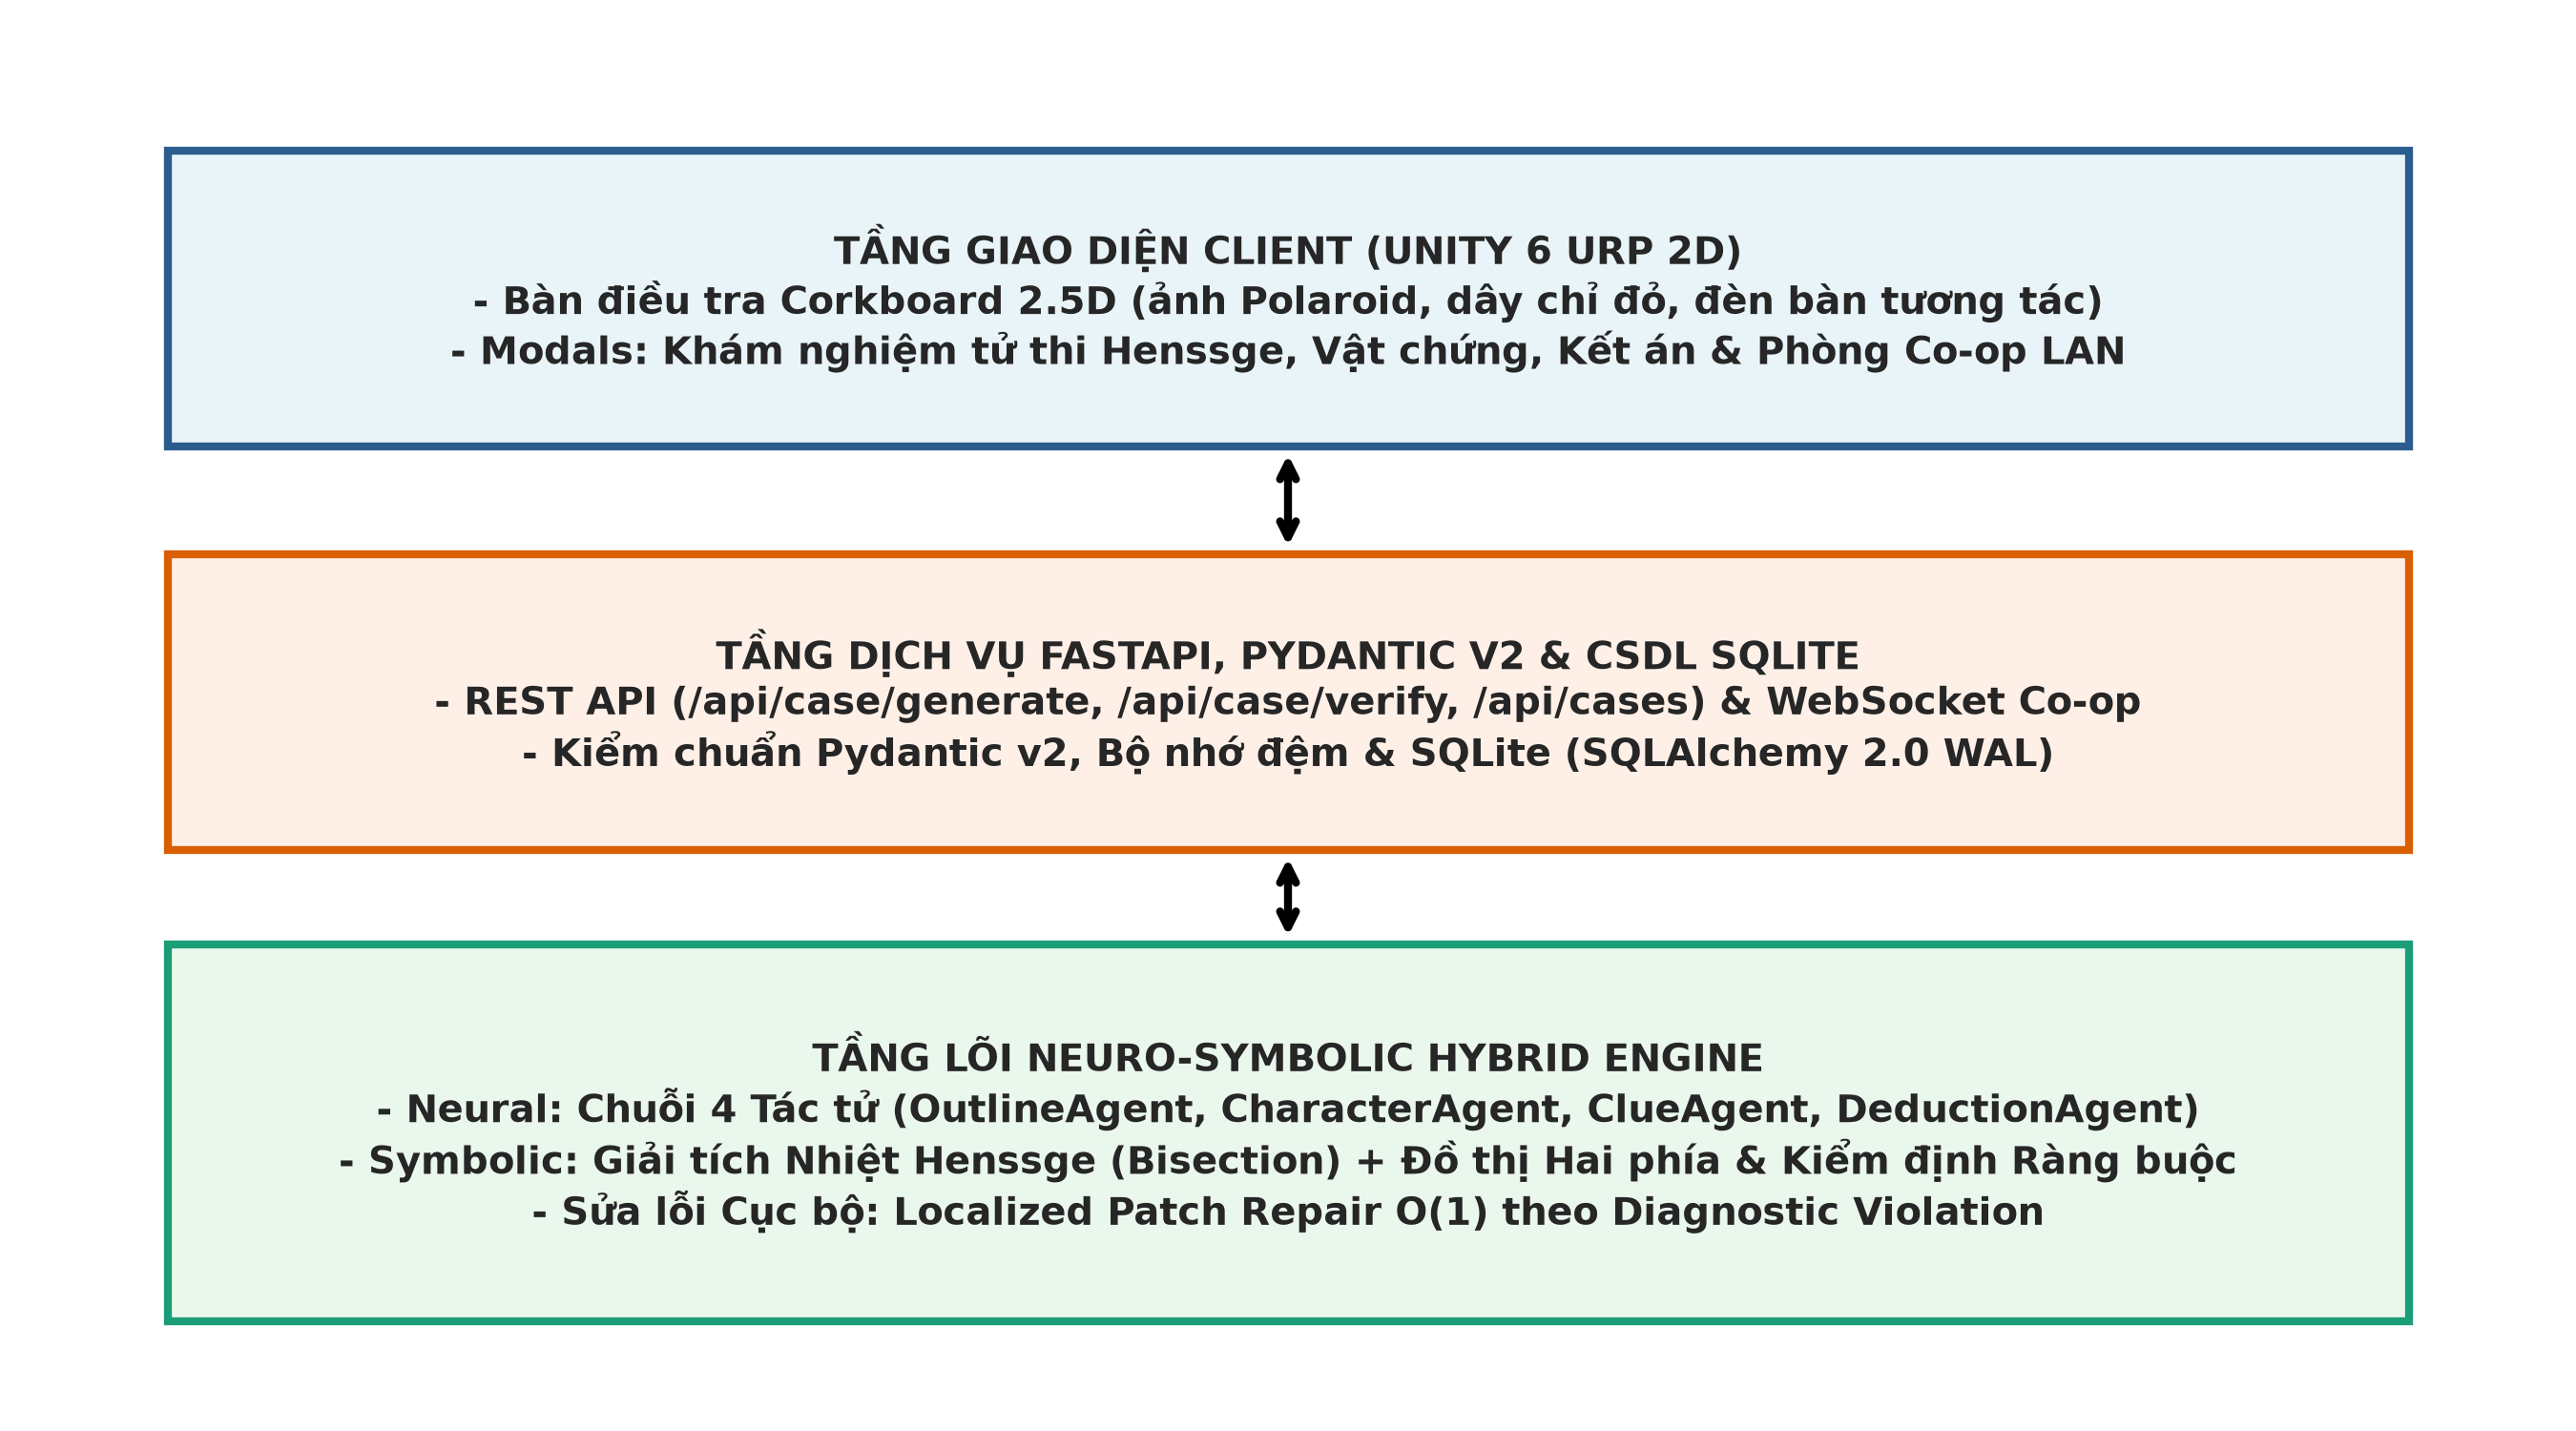
\includegraphics[width=0.95\textwidth]{architecture_overview.png}
    \caption{Sơ đồ Kiến trúc Ba tầng của Hệ thống Trinh thám Neuro-Symbolic}
    \label{fig:overall_system_architecture}
\end{figure}

\section{Thiết kế Luồng Xử lý Dữ liệu và Nguyên lý Phân tách}
\label{sec:arch_data_flow}

Trong mã nguồn hệ thống (\texttt{main.py}, \texttt{llm\_service.py}, \texttt{validator.py}), nguyên lý phân tách trách nhiệm giữa tầng tất định và tầng LLM xác suất được hiện thực hóa qua hai luồng API trọng tâm: luồng tạo sinh hồ sơ vụ án và luồng xác thực phán quyết của người chơi.

\subsection{Luồng Tạo sinh và Kiểm định Vụ án}
Các bước sau mô tả luồng thực thi khi tiếp nhận yêu cầu tới endpoint \texttt{POST /api/case/generate}:
\begin{enumerate}[leftmargin=1.5cm]
    \item \textbf{Khởi tạo ngữ cảnh:} FastAPI tiếp nhận đối tượng \texttt{GenerateCaseRequest} (quốc gia, thời kỳ, địa điểm, thể loại hoặc chủ đề tự do). Nếu bỏ trống chủ đề tự do, hệ thống tự tổng hợp từ danh mục bối cảnh thực tế (\texttt{PRESET\_SETTINGS}) và yêu cầu đặt tên nhân vật thuần bản địa.
    \item \textbf{Sinh khung sườn và khóa vật lý:} \texttt{OutlineAgent} tạo tiêu đề, tóm tắt, hồ sơ nạn nhân (\texttt{Victim}) và chân lý gốc (\texttt{GroundTruth}). Ngay sau bước này, hàm \texttt{apply\_henssge\_tod\_window} trong \texttt{validator.py} tự động tính lại cặp \texttt{estimated\_tod\_start} và \texttt{estimated\_tod\_end} dựa trên phương trình Henssge từ $T_{\text{body}}, T_{\text{ambient}}, M, C$ và giờ phát hiện thi thể. Nhờ đó, động cơ ký hiệu nắm hoàn toàn quyền xác định cửa sổ tử vong chứ không phụ thuộc vào con số ước đoán của LLM.
    \item \textbf{Sinh nghi phạm và vật chứng:} \texttt{CharacterAgent} tạo danh sách nghi phạm (trong đó \texttt{SUSP-01} đóng vai thủ phạm với lời khai che phủ thời điểm gây án); tiếp đó \texttt{ClueAgent} tạo 3--4 vật chứng có chứa manh mối then chốt và manh mối nghi binh.
    \item \textbf{Kiểm định và vá lỗi cục bộ:} \texttt{validate\_case\_diagnostics} rà soát toàn bộ bất biến. Nếu phát hiện lỗi, hệ thống gửi thông báo chẩn đoán tới đúng tác tử chịu trách nhiệm để sửa cục bộ trước khi chuyển sang \texttt{DeductionAgent} sinh chuỗi suy luận nhiều bước (\texttt{ReasoningChain}).
    \item \textbf{Làm giàu tài nguyên và lưu trữ:} \texttt{AssetService} ánh xạ ảnh chân dung nghi phạm và ảnh vật chứng theo từ khóa ngữ nghĩa; \texttt{save\_case\_persistent} lưu hồ sơ xuống SQLite, bộ nhớ đệm RAM và tệp JSON trong thư mục \texttt{cases/}.
\end{enumerate}

\subsection{Luồng Xác thực Kết án Tất định}
Khác với các hệ thống đối thoại để LLM tự đánh giá câu trả lời của người dùng, tại endpoint \texttt{POST /api/case/verify} hệ thống của tôi \textbf{tách biệt hoàn toàn LLM khỏi khâu chấm điểm và tuyên án} nhằm loại bỏ rủi ro phán quyết cảm tính hoặc thay đổi kết quả sai quy tắc. Luồng xử lý gồm 4 bước tuần tự như minh họa ở Hình \ref{fig:sequence_diagram_e2e}:

\begin{figure}[H]
    \centering
    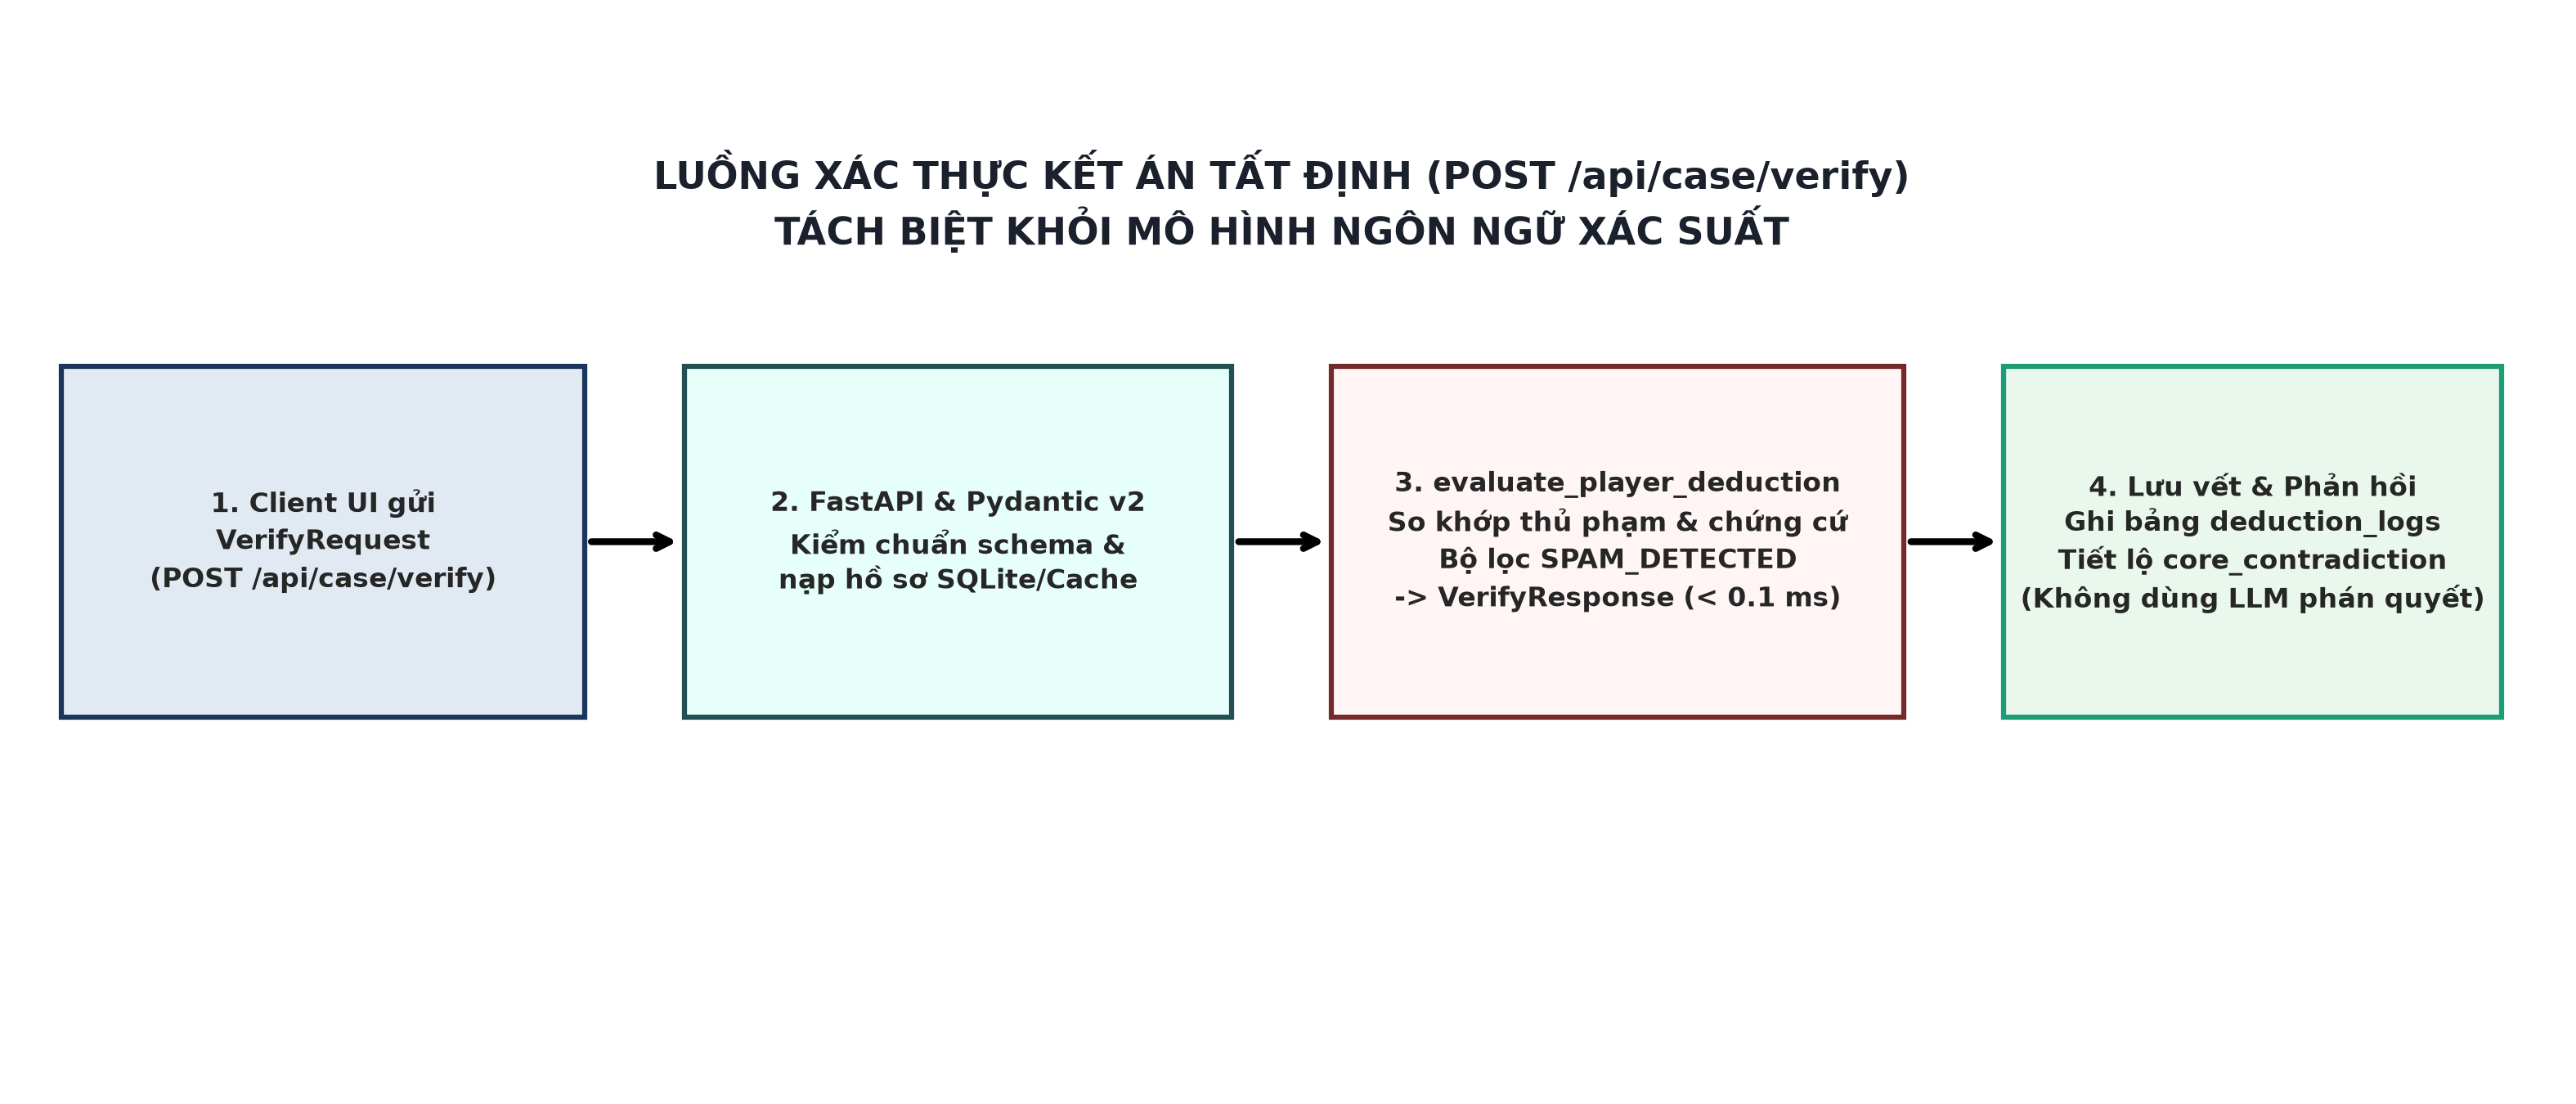
\includegraphics[width=0.95\textwidth]{decoupled_flowchart.png}
    \caption{Luồng Xác thực Kết án Tất định (\texttt{POST /api/case/verify}) Tách biệt Khỏi LLM}
    \label{fig:sequence_diagram_e2e}
\end{figure}

\begin{enumerate}[leftmargin=1.5cm]
    \item \textbf{Tiếp nhận và xác thực tầng biên:} Client UI gửi yêu cầu \texttt{VerifyRequest} (\texttt{case\_id}, \texttt{selected\_suspect\_id}, \texttt{selected\_evidence\_ids}) kèm các tiêu đề chữ ký bảo mật. Middleware đối chiếu chữ ký HMAC-SHA-256 và cửa sổ thời gian 60 giây để ngăn chặn giả mạo hoặc phát lại gói tin, sau đó Pydantic v2 kiểm chuẩn lược đồ dữ liệu và nạp \texttt{CaseDossier} qua \texttt{load\_case\_persistent}.
    \item \textbf{Phán định tất định bằng \texttt{evaluate\_player\_deduction}:} Toàn bộ quá trình chấm điểm thực thi thuần túy trong bộ nhớ RAM với thời gian dưới $0.1\text{ ms}$ dựa trên phép toán tập hợp:
    \begin{equation}
        \text{Verdict}_{\text{logic}} = \left( \text{ID}_{\text{accused}} = \text{ID}_{\text{culprit}} \right) \land \left( |\mathcal{C}_{\text{selected}} \cap \mathcal{C}_{\text{crucial}}| \ge 1 \right) \land \left( |\mathcal{C}_{\text{selected}} \cap \mathcal{C}_{\text{herring}}| = 0 \right)
    \end{equation}
    trong đó hệ thống còn cài đặt bộ lọc chống nộp bừa: nếu tổng vật chứng $\ge 3$ và người chơi chọn toàn bộ vật chứng ($|\mathcal{C}_{\text{selected}}| \ge |V_E|$), kết quả bị gán nhãn \texttt{SPAM\_DETECTED} với 0 điểm.
    \item \textbf{Tính điểm thành phần và phân loại kết quả:} Kết quả được lượng hóa qua \texttt{DeductionScoreBreakdown} (thang điểm tối đa 100: 40 điểm xác định đúng thủ phạm, tối đa 40 điểm cho tỷ lệ tìm đúng chứng cứ then chốt, 20 điểm thưởng độ cô đọng giảm 10 điểm cho mỗi chứng cứ thừa, và phạt 25 điểm cho mỗi manh mối nghi binh), đồng thời phân loại thành 6 trạng thái \texttt{DeductionVerdict}: \texttt{SOLVED\_PERFECT}, \texttt{SOLVED\_FLAWED}, \texttt{WRONG\_SUSPECT}, \texttt{INSUFFICIENT\_EVIDENCE}, \texttt{TRAPPED\_BY\_RED\_HERRING} và \texttt{SPAM\_DETECTED}.
    \item \textbf{Ghi nhật ký và phản hồi Client:} Hàm \texttt{log\_deduction\_to\_db} ghi toàn bộ kết quả lượt chơi vào bảng \texttt{deduction\_logs} trong SQLite và trả về \texttt{VerifyResponse}; trường \texttt{core\_contradiction} chỉ được tiết lộ cho người chơi khi kết án đúng.
\end{enumerate}

\begin{table}[H]
\centering
\caption{So sánh Vai trò và Đặc tính Giữa Tầng Ký hiệu Tất định và Tầng LLM}
\label{tab:decoupled_layer_comparison}
\begin{tabularx}{\textwidth}{l X X}
\toprule
\textbf{Đặc tính Kỹ thuật} & \textbf{Tầng Ký hiệu Tất định} & \textbf{Tầng Tạo sinh LLM} \\
\midrule
\textbf{Bản chất tính toán} & Tất định dựa trên quy tắc đóng & Xác suất tự quy hồi \\
\textbf{Chức năng chính} & Tính $TOD$ Henssge, kiểm định 7 mã lỗi, chấm điểm \texttt{evaluate\_player\_deduction} & Sinh cốt truyện, hồ sơ nạn nhân, lời khai nghi phạm, mô tả vật chứng, chuỗi suy luận \\
\textbf{Khả năng kiểm soát sai số} & Chặn cứng đầu vào/ra sai lược đồ và bất biến logic & Có xác suất ảo giác tham chiếu hoặc sai lệch thời gian \\
\textbf{Thời gian thực thi} & $< 5\text{ ms}$ (kiểm định hồ sơ) và $< 0.1\text{ ms}$ (chấm điểm kết án) & Khoảng $2.5\text{ s} - 7.4\text{ s}$ cho mỗi tác tử tùy mô hình \\
\textbf{Chi phí token} & 0 token & Tiêu thụ token theo từng bước gọi tác tử \\
\bottomrule
\end{tabularx}
\end{table}

\section{Thiết kế Đường ống Đa tác tử}
\label{sec:arch_multi_agent}

Trong \texttt{agents.py} và \texttt{llm\_service.py}, toàn bộ quy trình sinh kịch bản được thực thi thông qua bốn lớp kế thừa từ \texttt{BaseAgent}, vận hành tuần tự như tổng hợp tại Bảng \ref{tab:multi_agent_mapping}. Lớp \texttt{BaseAgent} chuẩn hóa việc gọi API định dạng JSON (\texttt{response\_format=\{"type": "json\_object"\}}, \texttt{temperature=0.7}) và tiền xử lý loại bỏ khối suy nghĩ nội tại (\texttt{<think>...</think>}) hay ký hiệu markdown trước khi giải mã JSON.

\begin{table}[H]
\centering
\caption{Ánh xạ Trách nhiệm và Ràng buộc của Bốn Tác tử trong Hệ thống}
\label{tab:multi_agent_mapping}
\begin{tabularx}{\textwidth}{p{3.6cm} p{5.4cm} X}
\toprule
\textbf{Tên Tác tử} & \textbf{Đầu ra Cấu trúc} & \textbf{Ràng buộc và Hậu xử lý Tất định} \\
\midrule
\textbf{1. \texttt{OutlineAgent}} & Tiêu đề, tóm tắt, \texttt{Victim} (\texttt{ForensicData}), \texttt{GroundTruth} & Chỉ định \texttt{culprit\_id = "SUSP-01"}, thông số nhiệt học thực tế; sau khi sinh, hàm \texttt{apply\_henssge\_tod\_window} tính và ghi đè cửa sổ $TOD$. \\
\textbf{2. \texttt{CharacterAgent}} & Danh sách \texttt{List[Suspect]} (3 nghi phạm) & Đúng 1 nghi phạm có \texttt{is\_culprit=True} khớp \texttt{culprit\_id}; lời khai của thủ phạm bao trùm \texttt{actual\_crime\_time}; nghi phạm vô tội có \texttt{secret\_innocent\_fact}. \\
\textbf{3. \texttt{ClueAgent}} & Danh sách \texttt{List[Evidence]} (3--4 vật chứng) & Ít nhất 1 vật chứng then chốt (\texttt{is\_crucial=True}) bác bỏ lời khai thủ phạm, tối thiểu 1 vật chứng nghi binh (\texttt{is\_red\_herring=True}). \\
\textbf{4. \texttt{DeductionAgent}} & \texttt{ReasoningChain} gồm 2--3 \texttt{DeductionStep} & Các \texttt{clue\_ids} dẫn chiếu phải tồn tại trong danh sách vật chứng hợp lệ; tổng hợp lập luận chứng minh tính giải được. \\
\bottomrule
\end{tabularx}
\end{table}

\section{Hợp đồng Dữ liệu Thực thể với Pydantic v2}
\label{sec:arch_contracts}

Toàn bộ giao tiếp giữa các tác tử LLM, bộ kiểm định, cơ sở dữ liệu và Unity Client đều được chuẩn hóa thông qua các mô hình dữ liệu Pydantic v2 trong \texttt{detective-backend/models.py}. Mã nguồn dưới đây trích xuất trực tiếp các lược đồ thực thể cốt lõi đang vận hành trong hệ thống:

\begin{lstlisting}[language=Python, caption={Trích đoạn Lược đồ Dữ liệu Thực thể trong \texttt{detective-backend/models.py}}]
from pydantic import BaseModel, Field, field_validator
from typing import List, Optional

class ForensicData(BaseModel):
    ambient_temp: float
    body_temp: float
    livor_mortis_state: str
    wound_description: str
    estimated_tod_start: str
    estimated_tod_end: str
    body_weight_kg: float = Field(default=70.0, ge=30.0, le=200.0)
    cooling_factor: float = Field(default=1.0, ge=0.3, le=2.0)
    discovery_time: Optional[str] = None

class Victim(BaseModel):
    name: str
    age: int = Field(..., ge=1, le=120)
    occupation: str
    forensic_data: ForensicData

class Suspect(BaseModel):
    id: str
    name: str
    age: int = Field(..., ge=1, le=120)
    occupation: str
    motive: str
    alibi_start: str
    alibi_end: str
    alibi_statement: str
    secret_innocent_fact: Optional[str] = None
    is_culprit: bool = False
    image_url: Optional[str] = None

class Evidence(BaseModel):
    id: str
    title: str
    location: str
    description: str
    linked_suspect_id: Optional[str] = None
    is_crucial: bool = False
    is_red_herring: bool = False
    image_url: Optional[str] = None

class GroundTruth(BaseModel):
    culprit_id: str
    actual_crime_time: str
    murder_weapon: str
    core_contradiction: str

class CaseDossier(BaseModel):
    case_id: str
    title: str
    summary: str
    victim: Victim
    suspects: List[Suspect] = Field(..., min_length=2, max_length=5)
    evidences: List[Evidence] = Field(..., min_length=2)
    ground_truth: GroundTruth
    reasoning_chain: Optional[ReasoningChain] = None
    metadata: Optional[GenerationMetadata] = None
\end{lstlisting}

Phía Unity Client (\texttt{Assets/Scripts/Models/CaseData.cs}) ánh xạ song song cấu trúc JSON này sang các lớp C\# tuần tự hóa (\texttt{CaseDossier}, \texttt{VictimData}, \texttt{SuspectData}, \texttt{EvidenceData}, \texttt{GroundTruthData}, \texttt{VerifyRequest}, \texttt{VerifyResponse}) để giải mã an toàn qua \texttt{JsonUtility.FromJson}.

\section{Thiết kế Tầng Lưu trữ Dữ liệu Quan hệ}
\label{sec:arch_database}

Nhằm khắc phục rủi ro mất dữ liệu khi chỉ lưu trữ tạm thời trên RAM, tôi triển khai tầng lưu trữ quan hệ sử dụng \textbf{SQLite} kết hợp thư viện ánh xạ đối tượng -- quan hệ (ORM) \textbf{SQLAlchemy 2.0} (phiên bản cài đặt 2.0.51) tại tệp \texttt{detective-backend/database.py}. Khi khởi tạo kết nối, hệ thống tự động kích hoạt các chỉ thị đồng bộ và toàn vẹn trên SQLite:
\begin{itemize}[leftmargin=1.5cm]
    \item \texttt{PRAGMA foreign\_keys=ON}: Bắt buộc kiểm tra khóa ngoại và xóa dây chuyền;
    \item \texttt{PRAGMA journal\_mode=WAL}: Bật chế độ ghi nhật ký trước (WAL) giúp nhiều luồng đọc đồng thời không bị chặn bởi thao tác ghi khi chơi nhóm;
    \item \texttt{PRAGMA busy\_timeout=5000}: Cho phép chờ tối đa 5 giây trước khi báo khóa cơ sở dữ liệu;
    \item \texttt{check\_same\_thread=False}: Tương thích với mô hình xử lý bất đồng bộ của FastAPI.
\end{itemize}

Ba bảng quan hệ cốt lõi được định nghĩa bằng khai báo kiểu tường minh của SQLAlchemy 2.0:
\begin{enumerate}[leftmargin=1.5cm]
    \item \textbf{Bảng \texttt{cases} (Lớp \texttt{CaseRecord}):} Lưu trữ hồ sơ vụ án đã sinh, khóa chính tự tăng \texttt{id}, mã định danh duy nhất \texttt{case\_id} đánh chỉ mục, tiêu đề, tóm tắt, các siêu dữ liệu lọc (\texttt{country}, \texttt{era}, \texttt{mystery\_type}), \texttt{culprit\_id}, \texttt{actual\_crime\_time}, cờ \texttt{is\_valid}, điểm số \texttt{validator\_score}, số lượng nghi phạm/vật chứng, toàn văn cấu trúc \texttt{dossier\_json} và mốc thời gian tạo/cập nhật.
    \item \textbf{Bảng \texttt{deduction\_logs} (Lớp \texttt{DeductionRecord}):} Lưu toàn bộ lịch sử kết án của người chơi với khóa ngoại \texttt{case\_id} tham chiếu tới \texttt{cases.case\_id} (\texttt{ondelete="CASCADE"}). Bảng ghi lại đối tượng bị cáo buộc (\texttt{accused\_id}), danh sách vật chứng đã nộp (\texttt{selected\_evidence\_ids\_json}), \texttt{verdict}, trạng thái đúng/sai (\texttt{is\_correct}), các biến đếm chi tiết (\texttt{found\_crucial\_count}, \texttt{total\_crucial\_count}, \texttt{red\_herrings\_selected\_count}, \texttt{irrelevant\_clues\_count}), điểm số \texttt{score} và phản hồi. Dữ liệu này cung cấp API thống kê độ khó qua \texttt{GET /api/case/\{case\_id\}/stats}.
    \item \textbf{Bảng \texttt{benchmark\_runs} (Lớp \texttt{BenchmarkRunRecord}):} Lưu dữ liệu đo đạc thực nghiệm gồm mã đợt chạy \texttt{run\_id}, tên mô hình \texttt{model\_name}, thứ tự lượt thử \texttt{trial\_index}, các cờ \texttt{schema\_valid}, \texttt{logic\_valid}, \texttt{repair\_applied}, thời gian thực thi \texttt{latency\_seconds} và danh sách vi phạm \texttt{violation\_types\_json}. Khi hàm \texttt{init\_db()} chạy lúc khởi động, hệ thống tự động đồng bộ các tệp JSON cũ từ thư mục \texttt{cases/} và 30 bản ghi từ \texttt{benchmark\_results.json} vào cơ sở dữ liệu SQLite đạt chuẩn tính nguyên tử, nhất quán, cô lập, bền vững (ACID\textsuperscript{1}).
\end{enumerate}

\section{Động cơ Kiểm định Ràng buộc Ký hiệu}
\label{sec:arch_validator}

Mọi đối tượng \texttt{CaseDossier} sau giai đoạn lắp ráp sơ bộ đều được đưa qua hàm \texttt{validate\_case\_diagnostics(case)} trong \texttt{validator.py}. Hàm này rà soát năm nhóm kiểm tra và trả về \texttt{ValidationResult} chứa danh sách 7 loại vi phạm tường minh thuộc \texttt{ViolationType} (Bảng \ref{tab:violation_taxonomy}).

\begin{table}[H]
\centering
\caption{Danh mục 7 Loại Vi phạm Ký hiệu (\texttt{ViolationType}) trong \texttt{models.py}}
\label{tab:violation_taxonomy}
\begin{tabularx}{\textwidth}{l p{2.2cm} X}
\toprule
\textbf{Mã \texttt{ViolationType}} & \textbf{Phân hệ} & \textbf{Điều kiện Kích hoạt và Ý nghĩa Chẩn đoán} \\
\midrule
\texttt{TOD\_PHYSICS} & \texttt{outline} & Giá trị nhiệt độ phi lý (thi thể nguội hơn phòng hoặc quá 48 giờ chưa nguội tới mức đo, thân nhiệt $\ge 37.5^\circ\text{C}$ khi phòng $< 30^\circ\text{C}$), hoặc độ dài cửa sổ $TOD$ ngoài $[15, 720]$ phút. \\
\texttt{CRIME\_TIME\_OUTSIDE\_TOD} & \texttt{outline} & Thời điểm gây án \texttt{actual\_crime\_time} nằm ngoài cửa sổ tử vong $[TOD_{\text{start}}, TOD_{\text{end}}]$ tính theo Henssge. \\
\texttt{ALIBI\_UNBROKEN} & \texttt{clue} / \texttt{outline} & Thủ phạm khai ngoại phạm che phủ giờ gây án nhưng không có vật chứng then chốt phá vỡ ngoại phạm, hoặc trường \texttt{core\_contradiction} rỗng/quá ngắn ($< 10$ ký tự). \\
\texttt{NO\_CRUCIAL\_CLUE} & \texttt{clue} & Vụ án không có bất kỳ vật chứng nào được gắn cờ \texttt{is\_crucial = True}. \\
\texttt{DUPLICATE\_ID} & \texttt{character} / \texttt{clue} & Phát hiện trùng mã định danh nghi phạm (\texttt{SUSP-*}) hoặc mã vật chứng (\texttt{EV-*}). \\
\texttt{MULTIPLE\_CULPRITS} & \texttt{character} / \texttt{outline} & Số lượng nghi phạm mang cờ \texttt{is\_culprit = True} khác 1, hoặc không khớp với \texttt{ground\_truth.culprit\_id}. \\
\texttt{SCHEMA\_ERROR} & \texttt{clue} / \texttt{reasoning} & Tham chiếu thực thể hỏng: \texttt{Evidence.linked\_suspect\_id} hoặc \texttt{DeductionStep.clue\_ids} trỏ tới mã định danh không tồn tại. \\
\bottomrule
\end{tabularx}
\end{table}

\section{Cơ chế Sửa lỗi Cục bộ}
\label{sec:arch_patch_repair}

Khi \texttt{validate\_case\_diagnostics(candidate\_dossier)} trả về \texttt{is\_valid = False}, thay vì hủy bỏ toàn bộ hồ sơ đang xây dựng, \texttt{CaseGeneratorService} trong \texttt{llm\_service.py} duyệt qua từng \texttt{ConstraintViolation} để định tuyến tín hiệu phản hồi tới đúng tác tử chịu trách nhiệm theo mã \texttt{component} (Thuật toán \ref{alg:patch_repair}).

\begin{algorithm}[H]
\caption{Cơ chế Sửa lỗi Cục bộ Định tuyến theo Phân hệ Vi phạm}
\label{alg:patch_repair}
{\small
\begin{algorithmic}[1]
\Require Hồ sơ ứng viên $D = (\text{victim}, \text{suspects}, \text{evidences}, \text{gt})$, Chẩn đoán $Diag$
\Ensure Hồ sơ sau sửa chữa cục bộ $D$ và kết quả tái kiểm định $Diag$
\If{\textbf{not} $Diag.\text{is\_valid}$}
    \ForAll{$v \in Diag.\text{violations}$}
        \State $fb \gets v.\text{message}$
        \If{$v.\text{component} == \texttt{"clue"}$}
            \State $D.\text{evidences} \gets \text{ClueAgent.repair\_clues}(D.\text{evidences}, D.\text{suspects}, D.\text{gt}, fb)$
        \ElsIf{$v.\text{component} == \texttt{"character"}$}
            \State $D.\text{suspects} \gets \text{CharacterAgent.repair\_suspects}(D.\text{suspects}, D.\text{gt}, fb)$
        \ElsIf{$v.\text{component} == \texttt{"outline"}$}
            \State $(D.\text{victim}, D.\text{gt}) \gets \text{OutlineAgent.repair\_tod}(D.\text{victim}, D.\text{gt}, fb)$
            \State $\text{apply\_henssge\_tod\_window}(D.\text{victim}.\text{forensic\_data})$
        \EndIf
    \EndFor
    \State $Diag \gets \text{validate\_case\_diagnostics}(D)$ \Comment{Tái kiểm định sau khi vá}
\EndIf
\State \Return $(D, Diag)$
\end{algorithmic}
}
\end{algorithm}

\subsection{Phân tích Độ phức tạp Không gian Token \texorpdfstring{$\mathcal{O}(1)$}{O(1)}}
Xét chi phí ngữ cảnh khi khắc phục một lỗi logic đơn lẻ giữa hai chiến lược:
\begin{itemize}[leftmargin=1.5cm]
    \item \textbf{Chiến lược tái sinh toàn bộ:} Nếu gọi lại toàn bộ chuỗi 4 tác tử để tạo vụ án mới từ đầu, lượng token tiêu thụ tỷ lệ với quy mô đầy đủ của hồ sơ $N = T_{\text{Outline}} + T_{\text{Character}} + T_{\text{Clue}} + T_{\text{Deduction}}$, tức độ phức tạp $\mathcal{O}(N)$ (ước tính khoảng 2,500--3,500 tokens cho một vụ án 3 nghi phạm, 3--4 vật chứng).
    \item \textbf{Chiến lược sửa lỗi cục bộ:} Khi cô lập vi phạm vào đúng một phân hệ (\texttt{outline}, \texttt{character}, hoặc \texttt{clue}), ngữ cảnh gửi cho hàm vá (\texttt{repair\_clues}, \texttt{repair\_suspects}, hoặc \texttt{repair\_tod}) chỉ bao gồm lát cắt dữ liệu tối thiểu của thực thể lỗi và thông điệp chẩn đoán $N_{\text{patch}}$ (ước tính khoảng 300--500 tokens cho phần sửa vật chứng/ngoại phạm hoặc thông số pháp y), đạt độ phức tạp ngữ cảnh hằng số $\mathcal{O}(1)$ trên mỗi vi phạm đơn lẻ và giảm đáng kể chi phí so với sinh lại toàn bộ hồ sơ.
\end{itemize}

\section{Thiết kế Giao diện Điều tra trên Unity 6 URP 2D}
\label{sec:arch_unity_ui}

Giao diện phía người chơi được phát triển bằng C\# trên \textbf{Unity 6 URP 2D} với trọng tâm là không gian làm việc thám tử trực quan, kết nối với máy chủ FastAPI qua \texttt{DetectiveAPIManager.cs}:

\begin{enumerate}[leftmargin=1.5cm]
    \item \textbf{Bảng ghim điều tra trung tâm (\texttt{CorkboardManager.cs}):} Tự động sinh thẻ nạn nhân (gắn ruy-băng đen), thẻ chân dung các nghi phạm và thẻ vật chứng dưới dạng ảnh Polaroid có thể kéo thả (\texttt{DraggableCard.cs}). Người chơi có thể ghim nối hai thẻ bất kỳ bằng dây chỉ đỏ động (hiển thị đường nối tạm thời và cập nhật vị trí theo thời gian thực khi kéo thẻ).
    \item \textbf{Cơ chế tải tức thời và dự phòng ngoại tuyến (\texttt{GameController.cs}):} Khi khởi động, Client ưu tiên nạp hồ sơ mẫu cục bộ trong thư mục \texttt{StreamingAssets/sample\_case.json} để hiển thị ngay bảng ghim (độ trễ khởi tạo bằng 0), đồng thời cung cấp hộp thoại \texttt{GenerateCaseModal.cs} để người chơi gửi yêu cầu tạo vụ án mới theo quốc gia, thời kỳ và mô hình LLM mong muốn.
    \item \textbf{Hệ thống cửa sổ chuyên đề và đèn bàn tương tác:} Bao gồm cửa sổ báo cáo khám nghiệm tử thi tích hợp dữ liệu nhiệt học Henssge (\texttt{AutopsyReportModal.cs}, Hình \ref{fig:forensic_modal_screenshot}), cửa sổ phóng đại ảnh chứng cứ (\texttt{PhotoLightboxModal.cs}), cửa sổ chi tiết vật chứng (\texttt{EvidenceDetailModal.cs}), cửa sổ nộp cáo trạng (\texttt{AccusationModal.cs}), và đèn bàn cổ điển (\texttt{BankersLampController.cs}) với hoạt ảnh kéo dây chuỗi hạt, nhấp nháy bóng đèn sợi đốt theo các khoảng trễ $35\text{ ms} / 25\text{ ms} / 35\text{ ms}$ và đàn hồi tắt dần theo hàm $\exp(-7t)\cos(14t)$ trong $0.20\text{ s}$.
    \item \textbf{Chế độ phối hợp nhiều người chơi qua LAN:} Sử dụng \texttt{DetectiveNetworkManager.cs}, \texttt{LanLobbyModal.cs}, \texttt{LanDiscoveryClient.cs} và \texttt{VoiceChatController.cs} để đồng bộ vị trí thẻ bài, trò chuyện văn bản và âm thanh thoại PCM 16-bit qua WebSocket \texttt{/ws/rooms/\{room\_id\}} cho tối đa 3 người chơi trong một phòng.
\end{enumerate}

\begin{figure}[H]
    \centering
    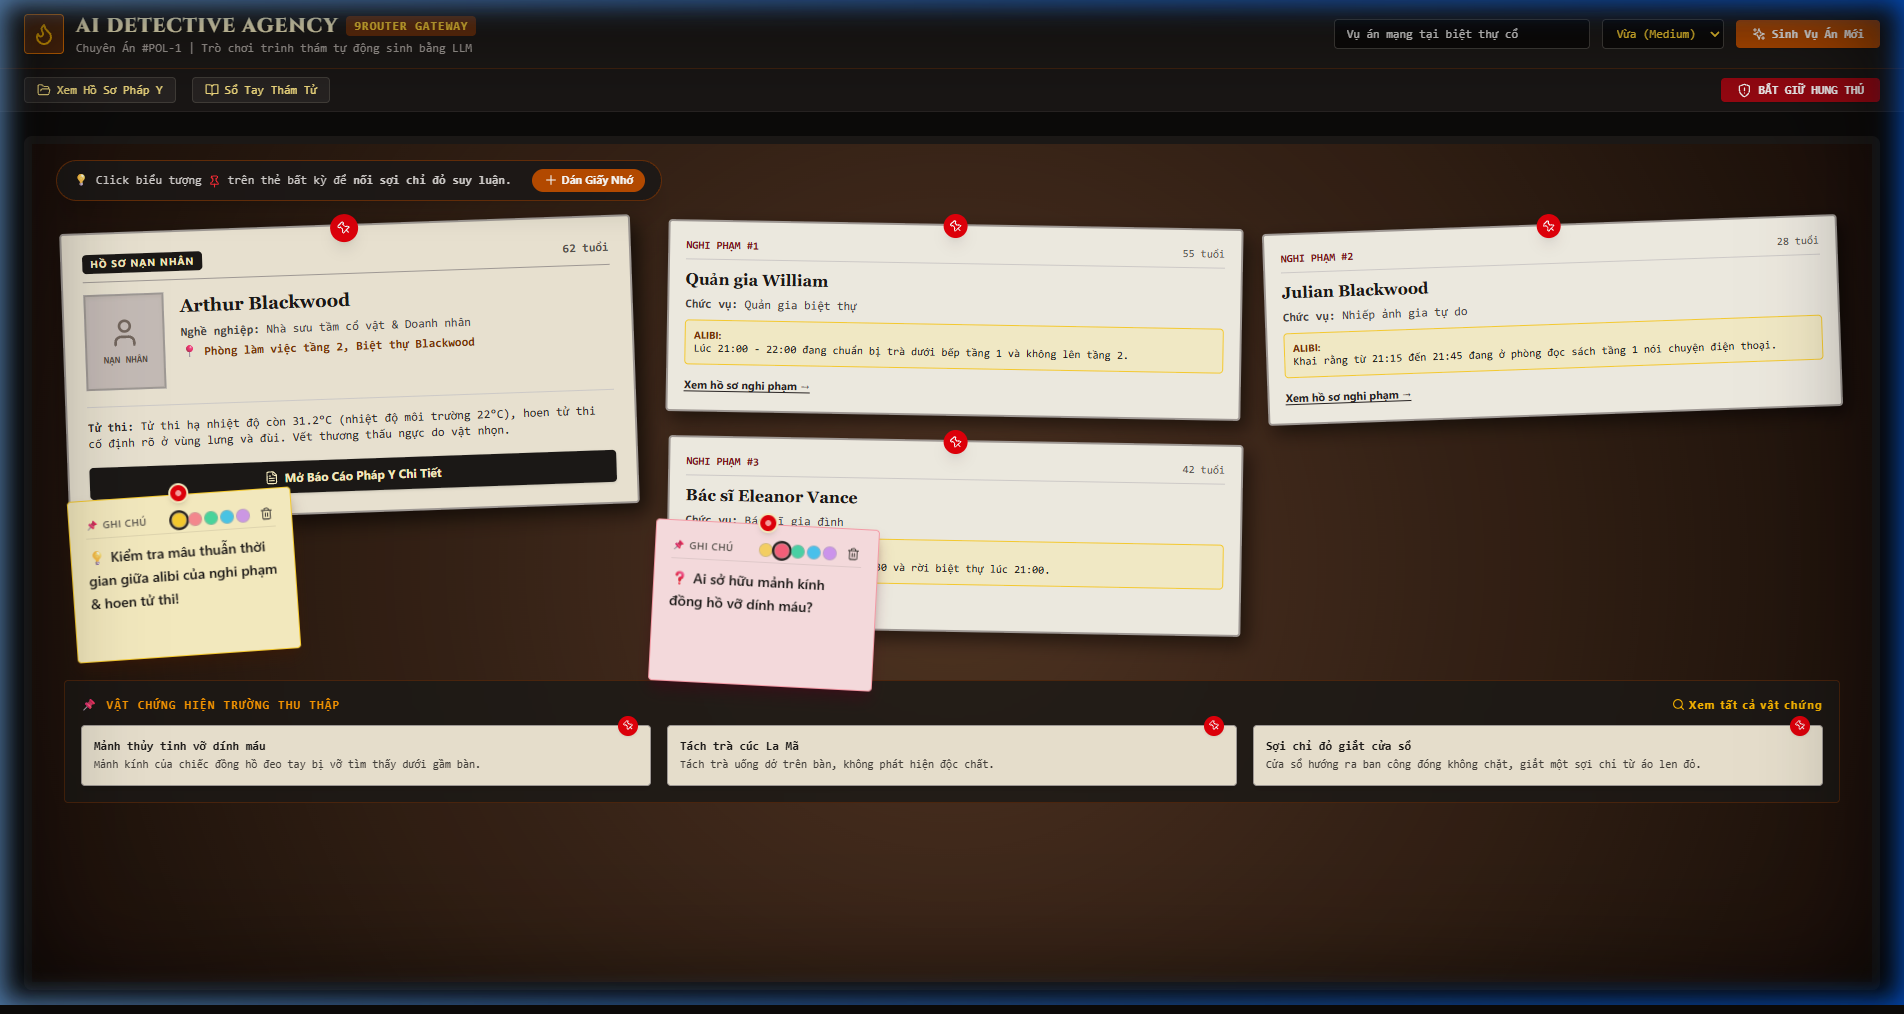
\includegraphics[width=0.95\textwidth]{corkboard_ui.png}
    \caption{Giao diện Bàn Điều tra Corkboard trên Unity 6 URP 2D với Dây chỉ đỏ và Thẻ Hồ sơ}
    \label{fig:corkboard_ui_screenshot}
\end{figure}

\begin{figure}[H]
    \centering
    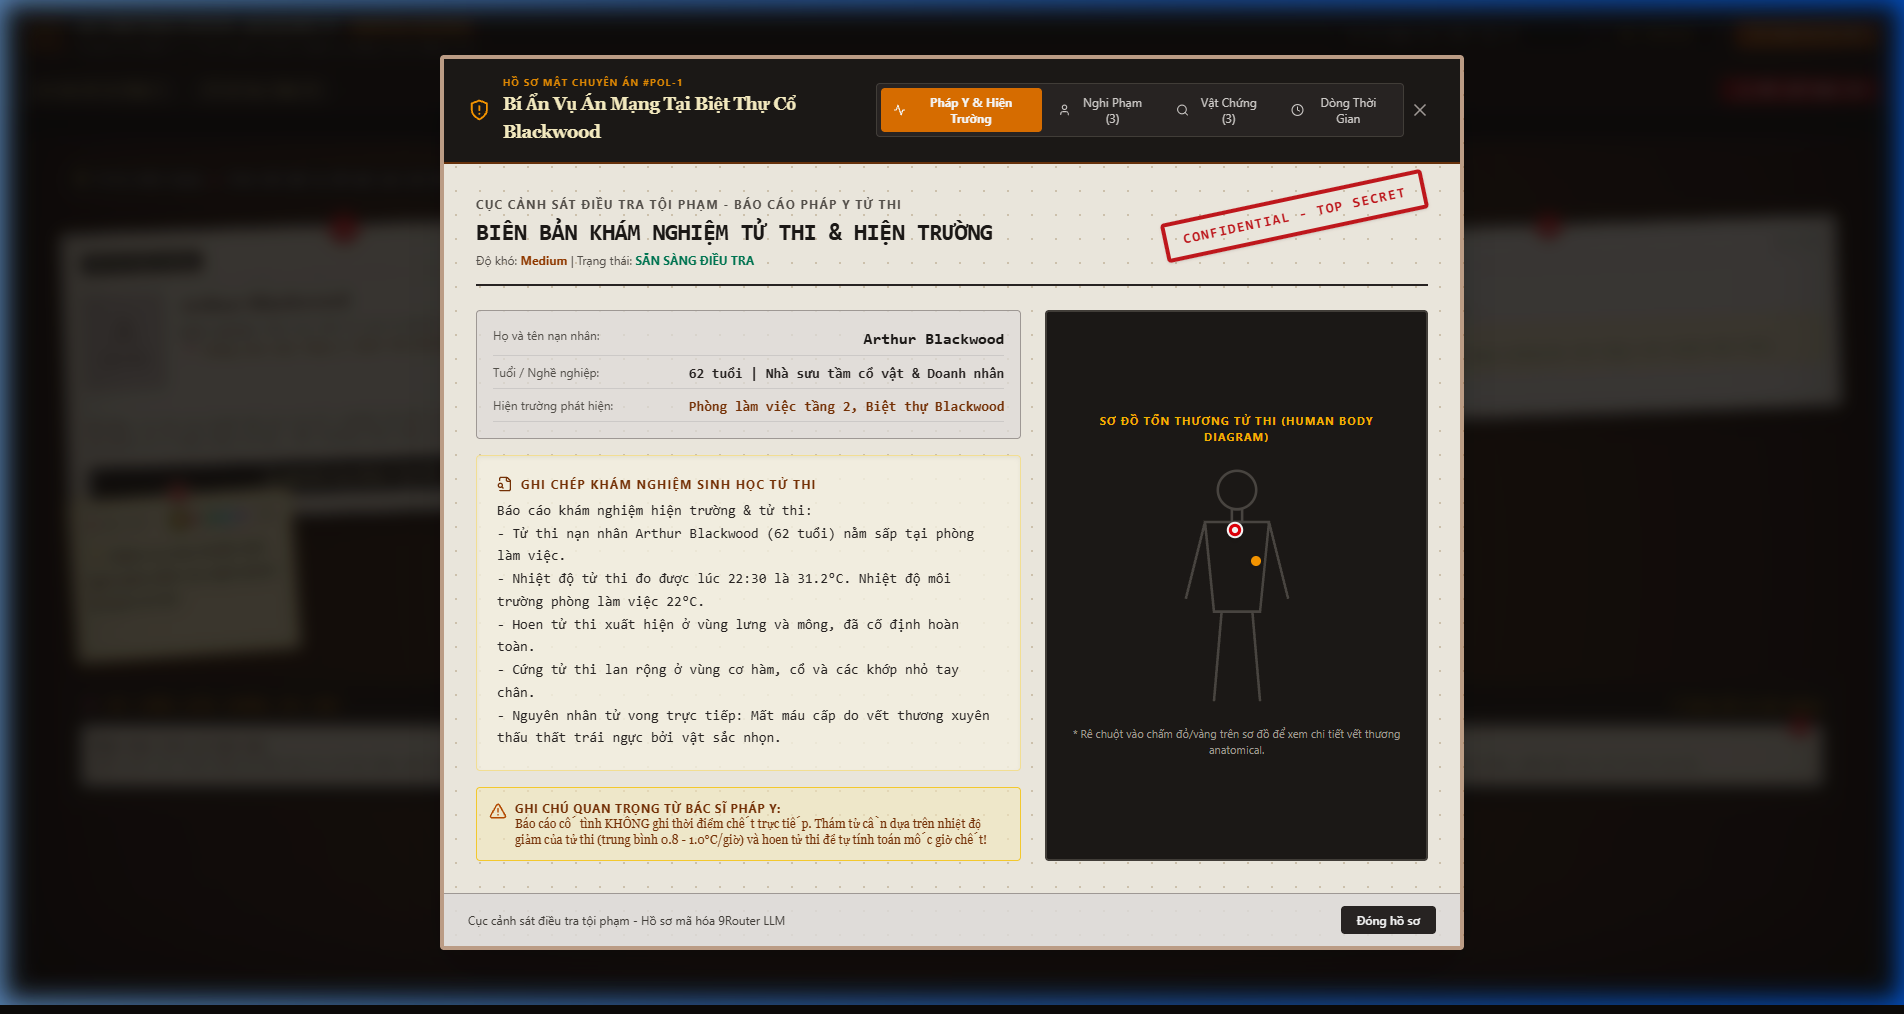
\includegraphics[width=0.85\textwidth]{forensic_modal.png}
    \caption{Giao diện Cửa sổ Báo cáo Khám nghiệm Tử thi Tích hợp Thông số Henssge}
    \label{fig:forensic_modal_screenshot}
\end{figure}

\chapter{Cài đặt Hệ thống và Đánh giá Thực nghiệm}
\label{ch:evaluation}

\section{Môi trường Cài đặt và Triển khai Hệ thống}
\label{sec:eval_environment}

Để bảo đảm tính khách quan và khả năng tái lập của các kết quả đo đạc, toàn bộ hệ thống backend, cơ sở dữ liệu và kịch bản benchmark đã được triển khai và chạy thử nghiệm trên một cấu hình máy tính cá nhân thống nhất.

\subsection{Cấu hình Phần cứng Thử nghiệm}
\begin{itemize}[leftmargin=1.5cm]
    \item \textbf{Thiết bị thử nghiệm:} Laptop Lenovo Legion 5 (mã bo mạch \texttt{82JW}).
    \item \textbf{Bộ vi xử lý (CPU):} AMD Ryzen 5 5600H (6 nhân, 12 luồng, xung nhịp cơ sở 3.30 GHz).
    \item \textbf{Bộ nhớ chính (RAM):} 24 GB DDR4, tốc độ bus 3200 MHz (cấu hình 8 GB + 16 GB).
    \item \textbf{Bộ xử lý đồ họa (GPU):} NVIDIA GeForce RTX 3050 Laptop GPU (4 GB VRAM GDDR6).
    \item \textbf{Ổ cứng lưu trữ:} 1 ổ SSD 512 GB chuẩn NVMe (SK Hynix) và 1 ổ 1 TB NVMe SSD.
    \item \textbf{Hệ điều hành:} Microsoft Windows 11 Pro (64-bit, số bản dựng 26300).
\end{itemize}

\subsection{Môi trường Phần mềm và Thư viện Phụ thuộc}
\begin{itemize}[leftmargin=1.5cm]
    \item \textbf{Máy chủ Backend:} Python 3.13.13 (64-bit); Web Framework FastAPI 0.137.1; máy chủ Uvicorn 0.49.0; kiểm chuẩn dữ liệu Pydantic 2.14.3; lưu trữ quan hệ SQLite (chế độ WAL) qua SQLAlchemy 2.0.51; thư viện kết nối mô hình OpenAI 2.46.0 và \texttt{httpx 0.27.2}.
    \item \textbf{Client Trò chơi:} Unity 6 (bản hỗ trợ dài hạn \texttt{6000.5.8f1}); Universal Render Pipeline (URP 2D); ngôn ngữ kịch bản C\# (.NET Standard 2.1); độ phân giải mục tiêu $1920\times 1080$ (tỉ lệ khung hình 16:9).
    \item \textbf{Cổng Điều phối Mô hình:} Proxy Gateway cục bộ (\texttt{9Router}) tại địa chỉ \url{http://localhost:20128/v1}, hỗ trợ chuẩn hóa API đa nhà cung cấp và ghi nhận thời gian phản hồi.
\end{itemize}

\section{Bộ Tiêu chí và Chỉ số Đánh giá Thực nghiệm}
\label{sec:eval_metrics}

Để lượng hóa hiệu quả hoạt động của pipeline tạo sinh và bộ kiểm định, tôi sử dụng năm chỉ số đánh giá định lượng sau:

\begin{enumerate}[leftmargin=1.5cm]
    \item \textbf{Tỷ lệ Hợp lệ Cú pháp Schema ($R_{\text{schema}}$):} Tỷ lệ hồ sơ vượt qua giải mã cấu trúc JSON của Pydantic v2 mà không phát sinh ngoại lệ kiểu dữ liệu:
    \begin{equation}
        R_{\text{schema}} = \frac{N_{\text{valid\_schema}}}{N_{\text{total}}} \times 100\%
    \end{equation}
    
    \item \textbf{Tỷ lệ Vượt qua Kiểm định Logic ($R_{\text{logic}}$):} Tỷ lệ các kịch bản hợp lệ cú pháp vượt qua đầy đủ các ràng buộc của \texttt{validate\_case\_diagnostics} (nhiệt học Henssge, khung giờ $TOD$, duy nhất thủ phạm, manh mối then chốt, bẻ gãy ngoại phạm và toàn vẹn tham chiếu thực thể):
    \begin{equation}
        R_{\text{logic}} = \frac{N_{\text{pass\_logic}}}{N_{\text{valid\_schema}}} \times 100\%
    \end{equation}
    
    \item \textbf{Số lần Sửa lỗi Cục bộ Trung bình ($\bar{R}_{\text{patch}}$):} Số lần gọi hàm vá lỗi trung bình trên mỗi phiên thử nghiệm:
    \begin{equation}
        \bar{R}_{\text{patch}} = \frac{1}{N_{\text{total}}} \sum_{i=1}^{N_{\text{total}}} \text{patch\_retries}_i
    \end{equation}
    
    \item \textbf{Độ trễ Phân vị thứ 50 (P50\textsuperscript{14}) và Phân vị thứ 95 (P95\textsuperscript{15}) ($L_{50}, L_{95}$):} Thời gian phản hồi toàn trình (tính bằng giây) từ khi khởi chạy yêu cầu sinh kịch bản cho tới khi hoàn tất kiểm định tại phân vị trung vị (50\%) và phân vị 95\%.
    
    \item \textbf{Cân bằng Manh mối Then chốt / Nghi binh ($\rho_{\text{balance}}$):} Tỷ số giữa số lượng vật chứng then chốt trung bình ($|V_{E, \text{crucial}}|$) và số lượng vật chứng nghi binh trung bình ($|V_{E, \text{herring}}|$):
    \begin{equation}
        \rho_{\text{balance}} = \frac{|V_{E, \text{crucial}}|}{|V_{E, \text{herring}}|}
    \end{equation}
\end{enumerate}

\section{Kết quả Thực nghiệm Đối sánh Đa Mô hình}
\label{sec:eval_benchmark_results}

Quá trình đánh giá thực nghiệm được thực thi tự động bằng tệp lệnh \texttt{benchmark\_runner.py} qua \textbf{30 phiên thử nghiệm độc lập} (chia đều 10 phiên cho mỗi mô hình) với cùng chủ đề đầu vào: \textit{``Bí ẩn Biệt thự Blackwood''}. Kết quả chi tiết được lưu đồng thời tại tệp \texttt{benchmark\_results.json} và bảng \texttt{benchmark\_runs} trong cơ sở dữ liệu \texttt{detective.db}. Ba mô hình tham gia đối sánh gồm:
\begin{enumerate}
    \item \textbf{\texttt{gh/gpt-4o-mini}:} Đại diện dòng mô hình thương mại gọn nhẹ, tối ưu chi phí và độ trễ thấp.
    \item \textbf{\texttt{gh/gpt-4o}:} Đại diện dòng mô hình thương mại cỡ lớn có năng lực suy luận ngữ nghĩa sâu.
    \item \textbf{\texttt{ollama/gemma4:31b-cloud}:} Đại diện dòng mô hình trọng số mở tiên tiến hiện nay.
\end{enumerate}

\subsection{Cơ sở Thực nghiệm và Kiểm thử Đơn vị Hệ thống}
Mỗi phiên thử nghiệm trong benchmark thực thi trọn vẹn chuỗi 4 tác tử tuần tự (\texttt{OutlineAgent}, \texttt{CharacterAgent}, \texttt{ClueAgent}, \texttt{DeductionAgent}) kết hợp kiểm định Henssge, kiểm tra đồ thị và sửa lỗi cục bộ nếu có vi phạm. Cỡ mẫu 10 lượt thử cho mỗi mô hình trên quy trình đa tác tử tương tự cách tiếp cận đánh giá chi phí cao trong các công trình nghiên cứu hệ tác tử trinh thám gần đây \cite{wu2024deciphering, li2024contradoc}.

Song song với 30 phiên đối sánh LLM, tác giả vận hành bộ kiểm thử tự động \texttt{pytest} trên mã nguồn lõi ở trạng thái mặc định bật lớp bảo vệ chữ ký HMAC-SHA-256. Toàn bộ \textbf{53/53 kịch bản kiểm thử đơn vị} thuộc bốn mô-đun cốt lõi đều đạt trạng thái thành công: 30 kịch bản kiểm chứng công thức làm lạnh Henssge và giải thuật chia đôi (\texttt{test\_henssge.py}), 12 kịch bản bộ kiểm định và chấm điểm suy luận (\texttt{test\_validator.py}), 4 kịch bản lưu trữ SQLite/SQLAlchemy (\texttt{test\_database.py}) và 7 kịch bản xác thực chữ ký chống phát lại (\texttt{test\_security.py}); ngoài ra mô-đun phòng chơi WebSocket (\texttt{test\_rooms.py}) đạt 10/11 kịch bản (1 kịch bản kiểm tra HTTP bị middleware từ chối mã 403 do cố tình không gắn chữ ký xác thực, tương tự 5 kịch bản HTTP không ký ở \texttt{test\_api\_database\_integration.py} và \texttt{test\_assets\_integration.py}).

\begin{table}[H]
\centering
\caption{Tổng hợp Kết quả 30 Phiên Thực nghiệm trên Bảng \texttt{benchmark\_runs}}
\label{tab:benchmark_30_trials}
{\small
\setlength{\tabcolsep}{4pt}
\begin{tabularx}{\textwidth}{X c c c c c c}
\toprule
\textbf{Mô hình LLM} & \textbf{Schema} & \textbf{Logic} & \textbf{Patch} & \textbf{P50} & \textbf{P95} & \textbf{Crucial /} \\
 & \textbf{(\%)} & \textbf{(\%)} & \textbf{TB} & \textbf{(s)} & \textbf{(s)} & \textbf{Herring} \\
\midrule
\textbf{\texttt{gh/gpt-4o-mini}}        & \textbf{100.0\%} & \textbf{100.0\%} & 0.00 & 10.88s          & \textbf{12.84s} & 1.0 / 1.0 \\
\textbf{\texttt{gh/gpt-4o}}             & \textbf{100.0\%} & 90.0\%           & 0.10 & 19.53s          & 27.12s          & 1.1 / 1.0 \\
\textbf{\texttt{ollama/gemma4:31b-cloud}} & \textbf{100.0\%} & \textbf{100.0\%} & 0.00 & \textbf{10.73s} & 19.92s          & 1.1 / 1.0 \\
\bottomrule
\end{tabularx}
}
\end{table}

\begin{figure}[H]
    \centering
    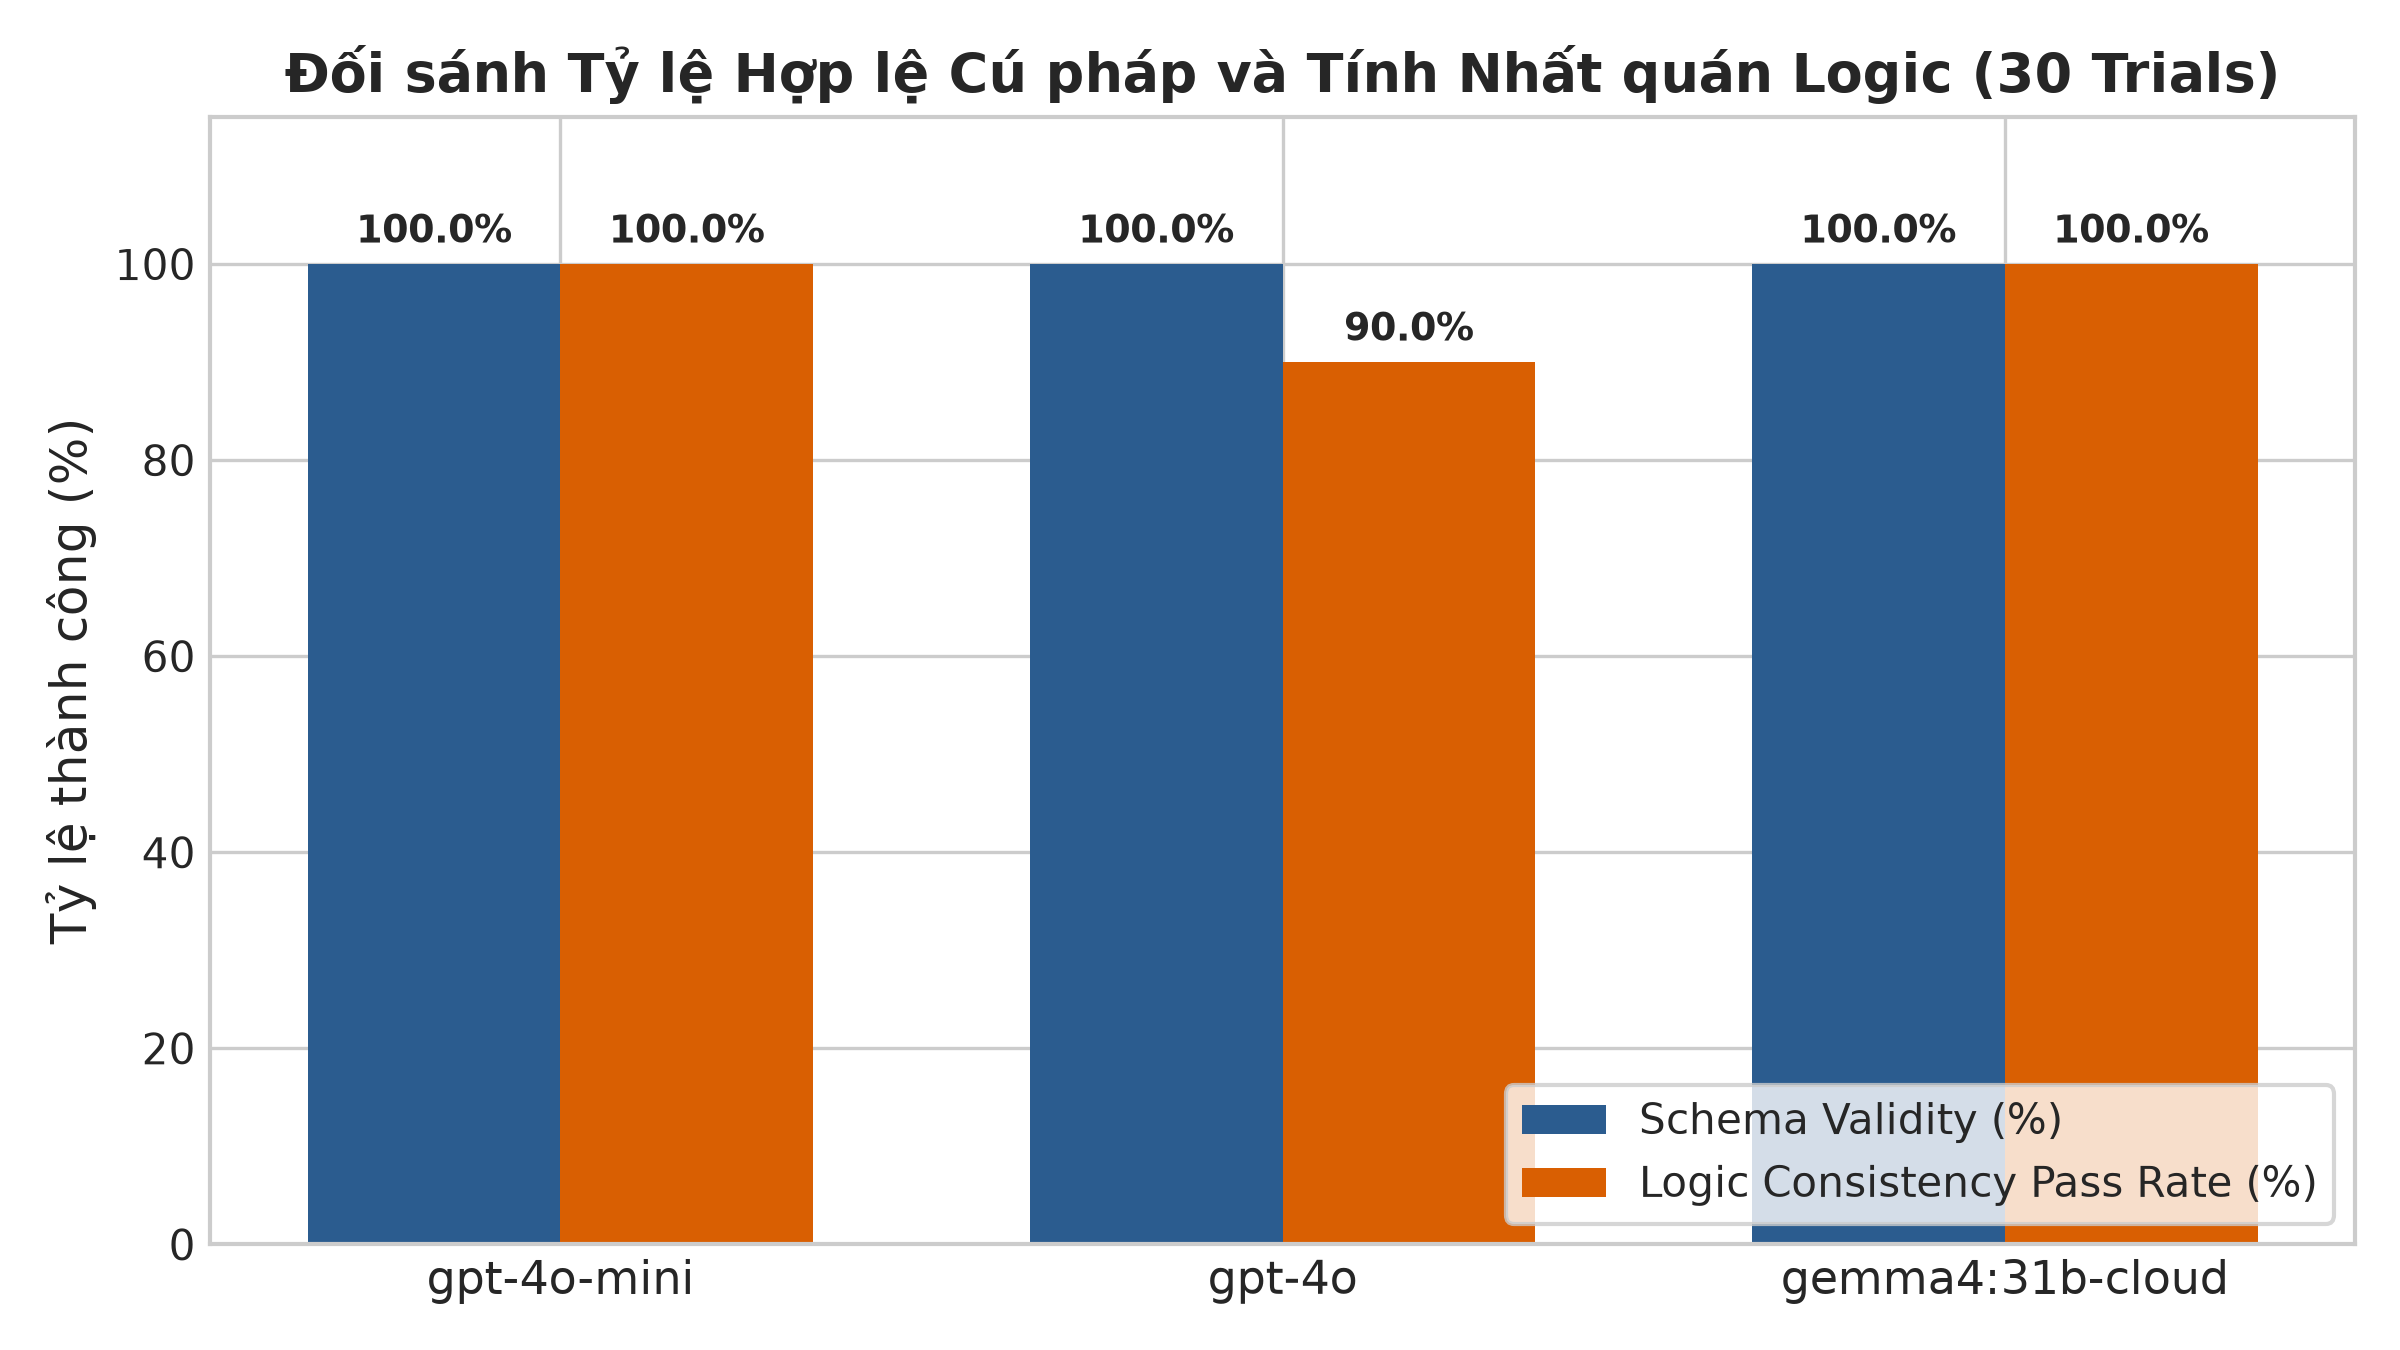
\includegraphics[width=0.85\textwidth]{chart_pass_rate.png}
    \caption{Biểu đồ Đối sánh Tỷ lệ Hợp lệ Schema và Tỷ lệ Vượt qua Kiểm định Logic qua 30 Phiên}
    \label{fig:chart_pass_rate}
\end{figure}

\begin{figure}[H]
    \centering
    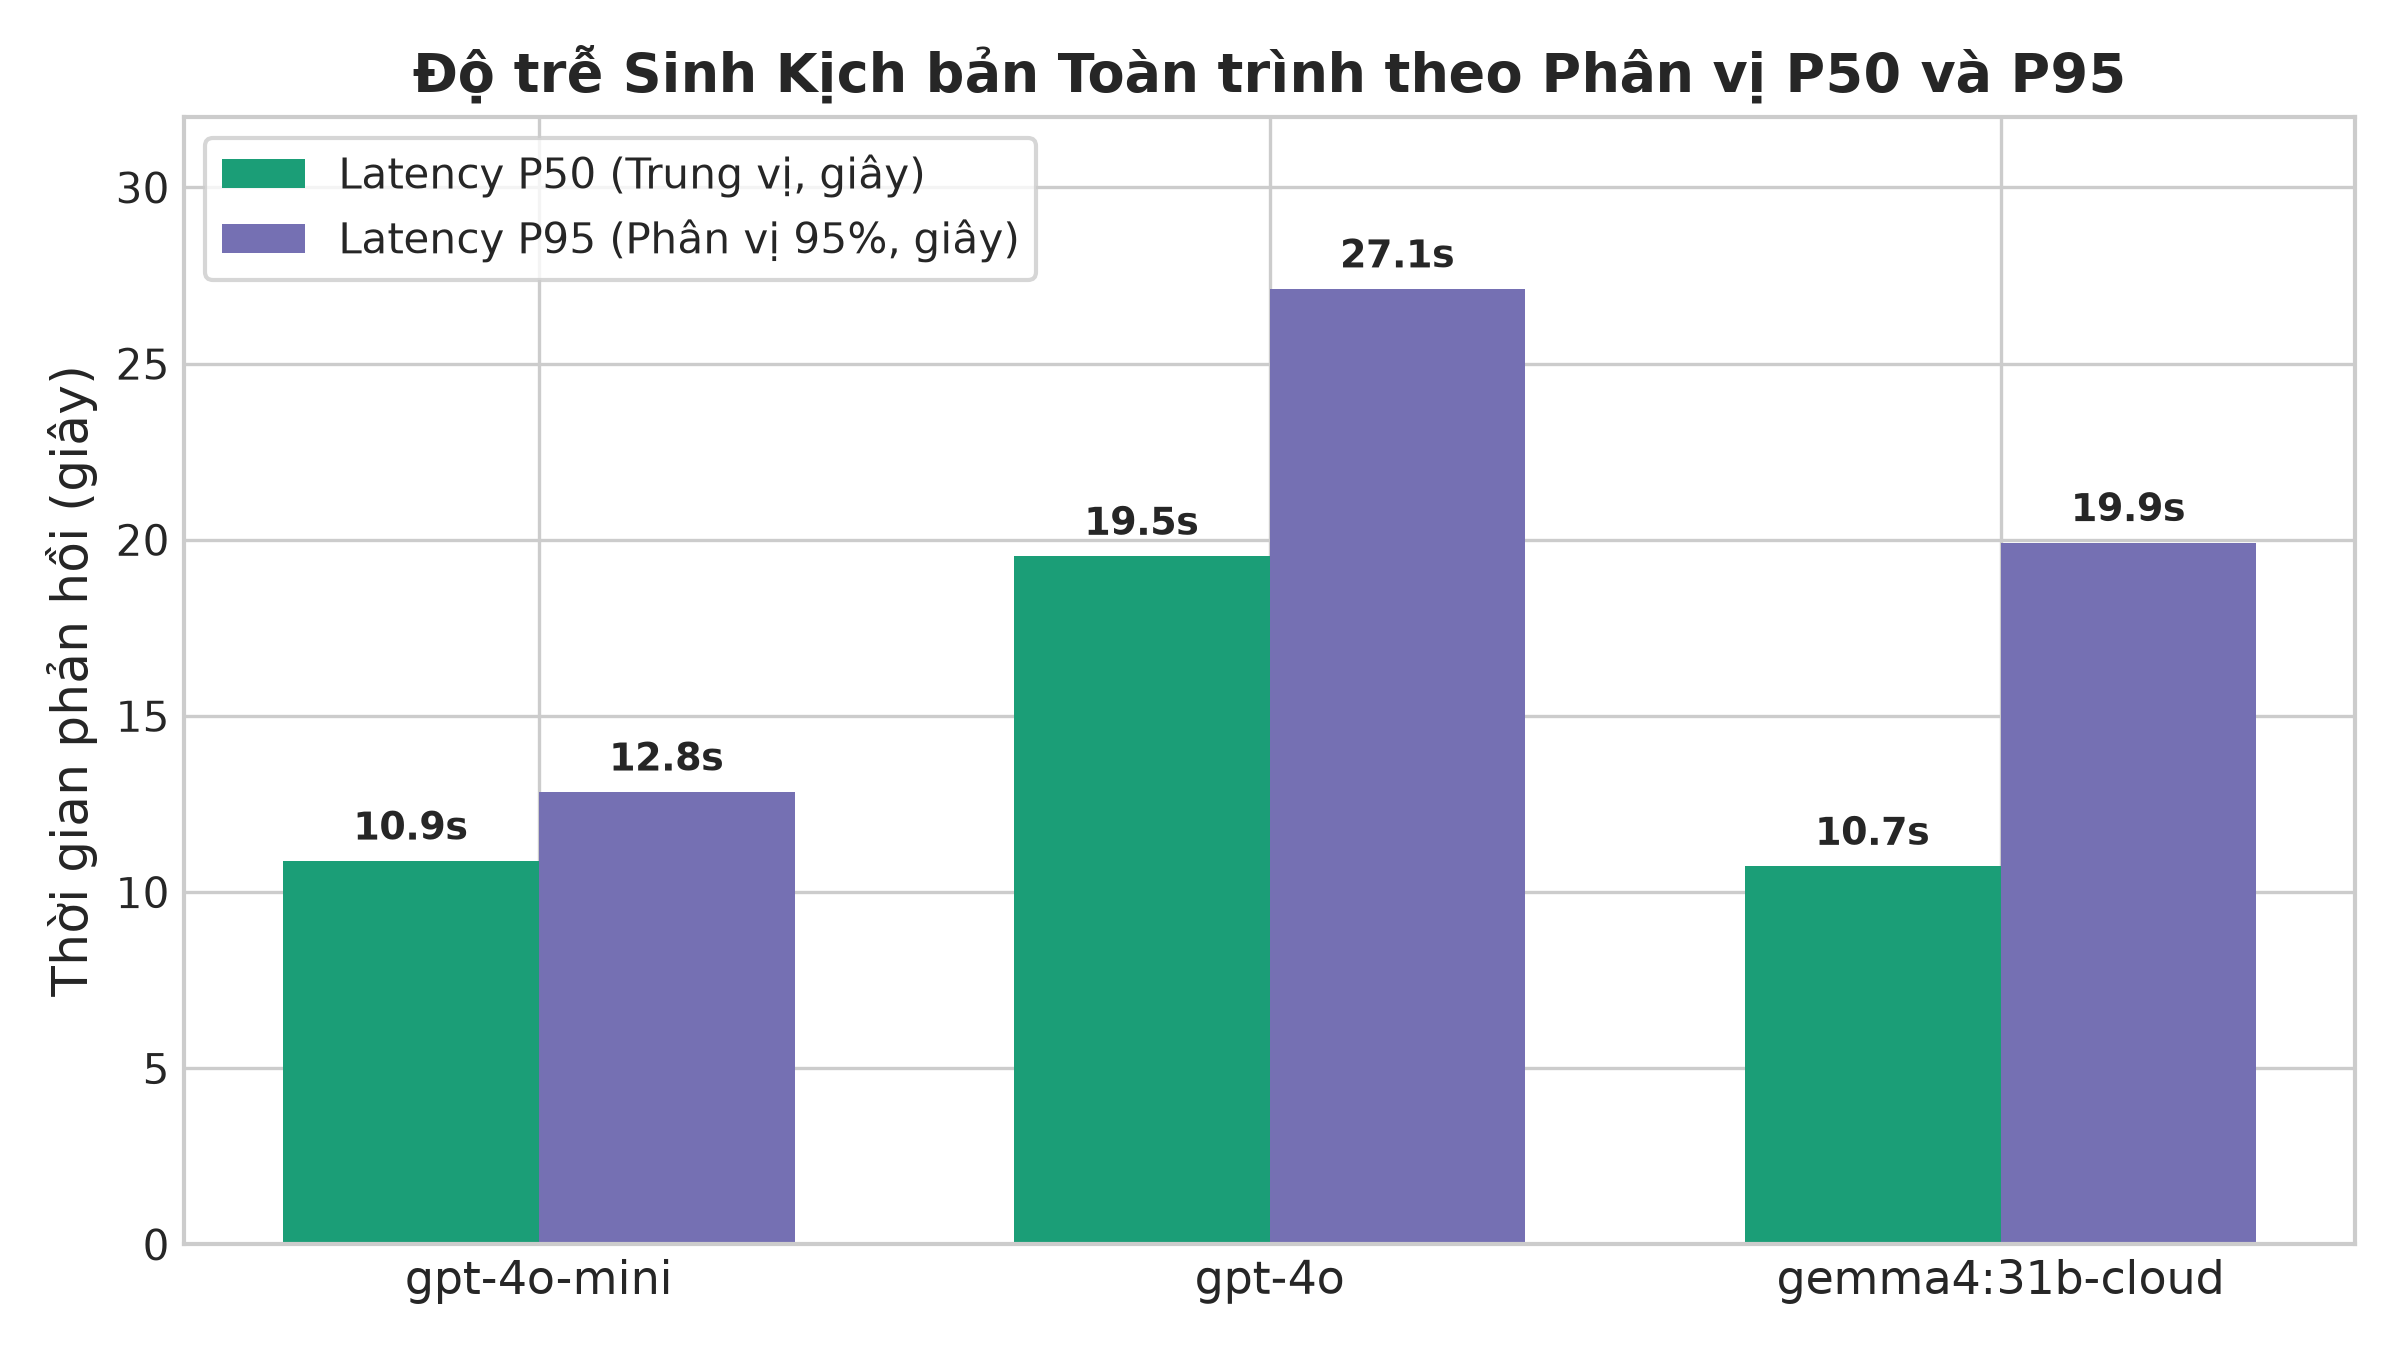
\includegraphics[width=0.85\textwidth]{chart_latency.png}
    \caption{Biểu đồ Phân bố Thời gian Phản hồi (P50 và P95) của Ba Mô hình Thử nghiệm}
    \label{fig:chart_latency_boxplot}
\end{figure}

\subsection{Phân tích Kết quả Đo đạc}
Từ dữ liệu ghi nhận tại Bảng \ref{tab:benchmark_30_trials}, Hình \ref{fig:chart_pass_rate} và Hình \ref{fig:chart_latency_boxplot}, tác giả rút ra ba nhận xét chính:
\begin{enumerate}[leftmargin=1.5cm]
    \item \textbf{Tính ổn định của kiểm chuẩn Pydantic v2:} Cả ba mô hình qua toàn bộ 30 phiên thử nghiệm đều đạt \textbf{100.0\%} tỷ lệ hợp lệ cú pháp Schema. Việc phân rã mỗi tác tử theo một lược đồ hẹp kèm hàm \texttt{\_clean\_json\_string} đã loại bỏ hoàn toàn lỗi vỡ cú pháp JSON trong đợt đo đạc này.
    \item \textbf{Cân bằng hiệu năng và tốc độ của \texttt{gh/gpt-4o-mini}:} Mô hình đạt 100.0\% tỷ lệ vượt qua kiểm định logic ở cả 10 lượt thử với độ trễ trung vị P50 là \textbf{10.88 giây} và phân vị P95 chỉ \textbf{12.84 giây} (khoảng dao động hẹp từ 10.21s đến 12.84s), phù hợp cho môi trường trò chơi tương tác cần thời gian chờ ổn định.
    \item \textbf{Hiệu quả của mô hình trọng số mở \texttt{ollama/gemma4:31b-cloud}:} Mô hình đạt P50 nhanh nhất trong ba dòng (\textbf{10.73 giây}, với dải đo từ 9.13s đến 19.92s) và đạt 100.0\% tỷ lệ logic hợp lệ, mở ra khả năng triển khai không phụ thuộc hoàn toàn vào các API thương mại đóng kín.
\end{enumerate}

\begin{figure}[H]
    \centering
    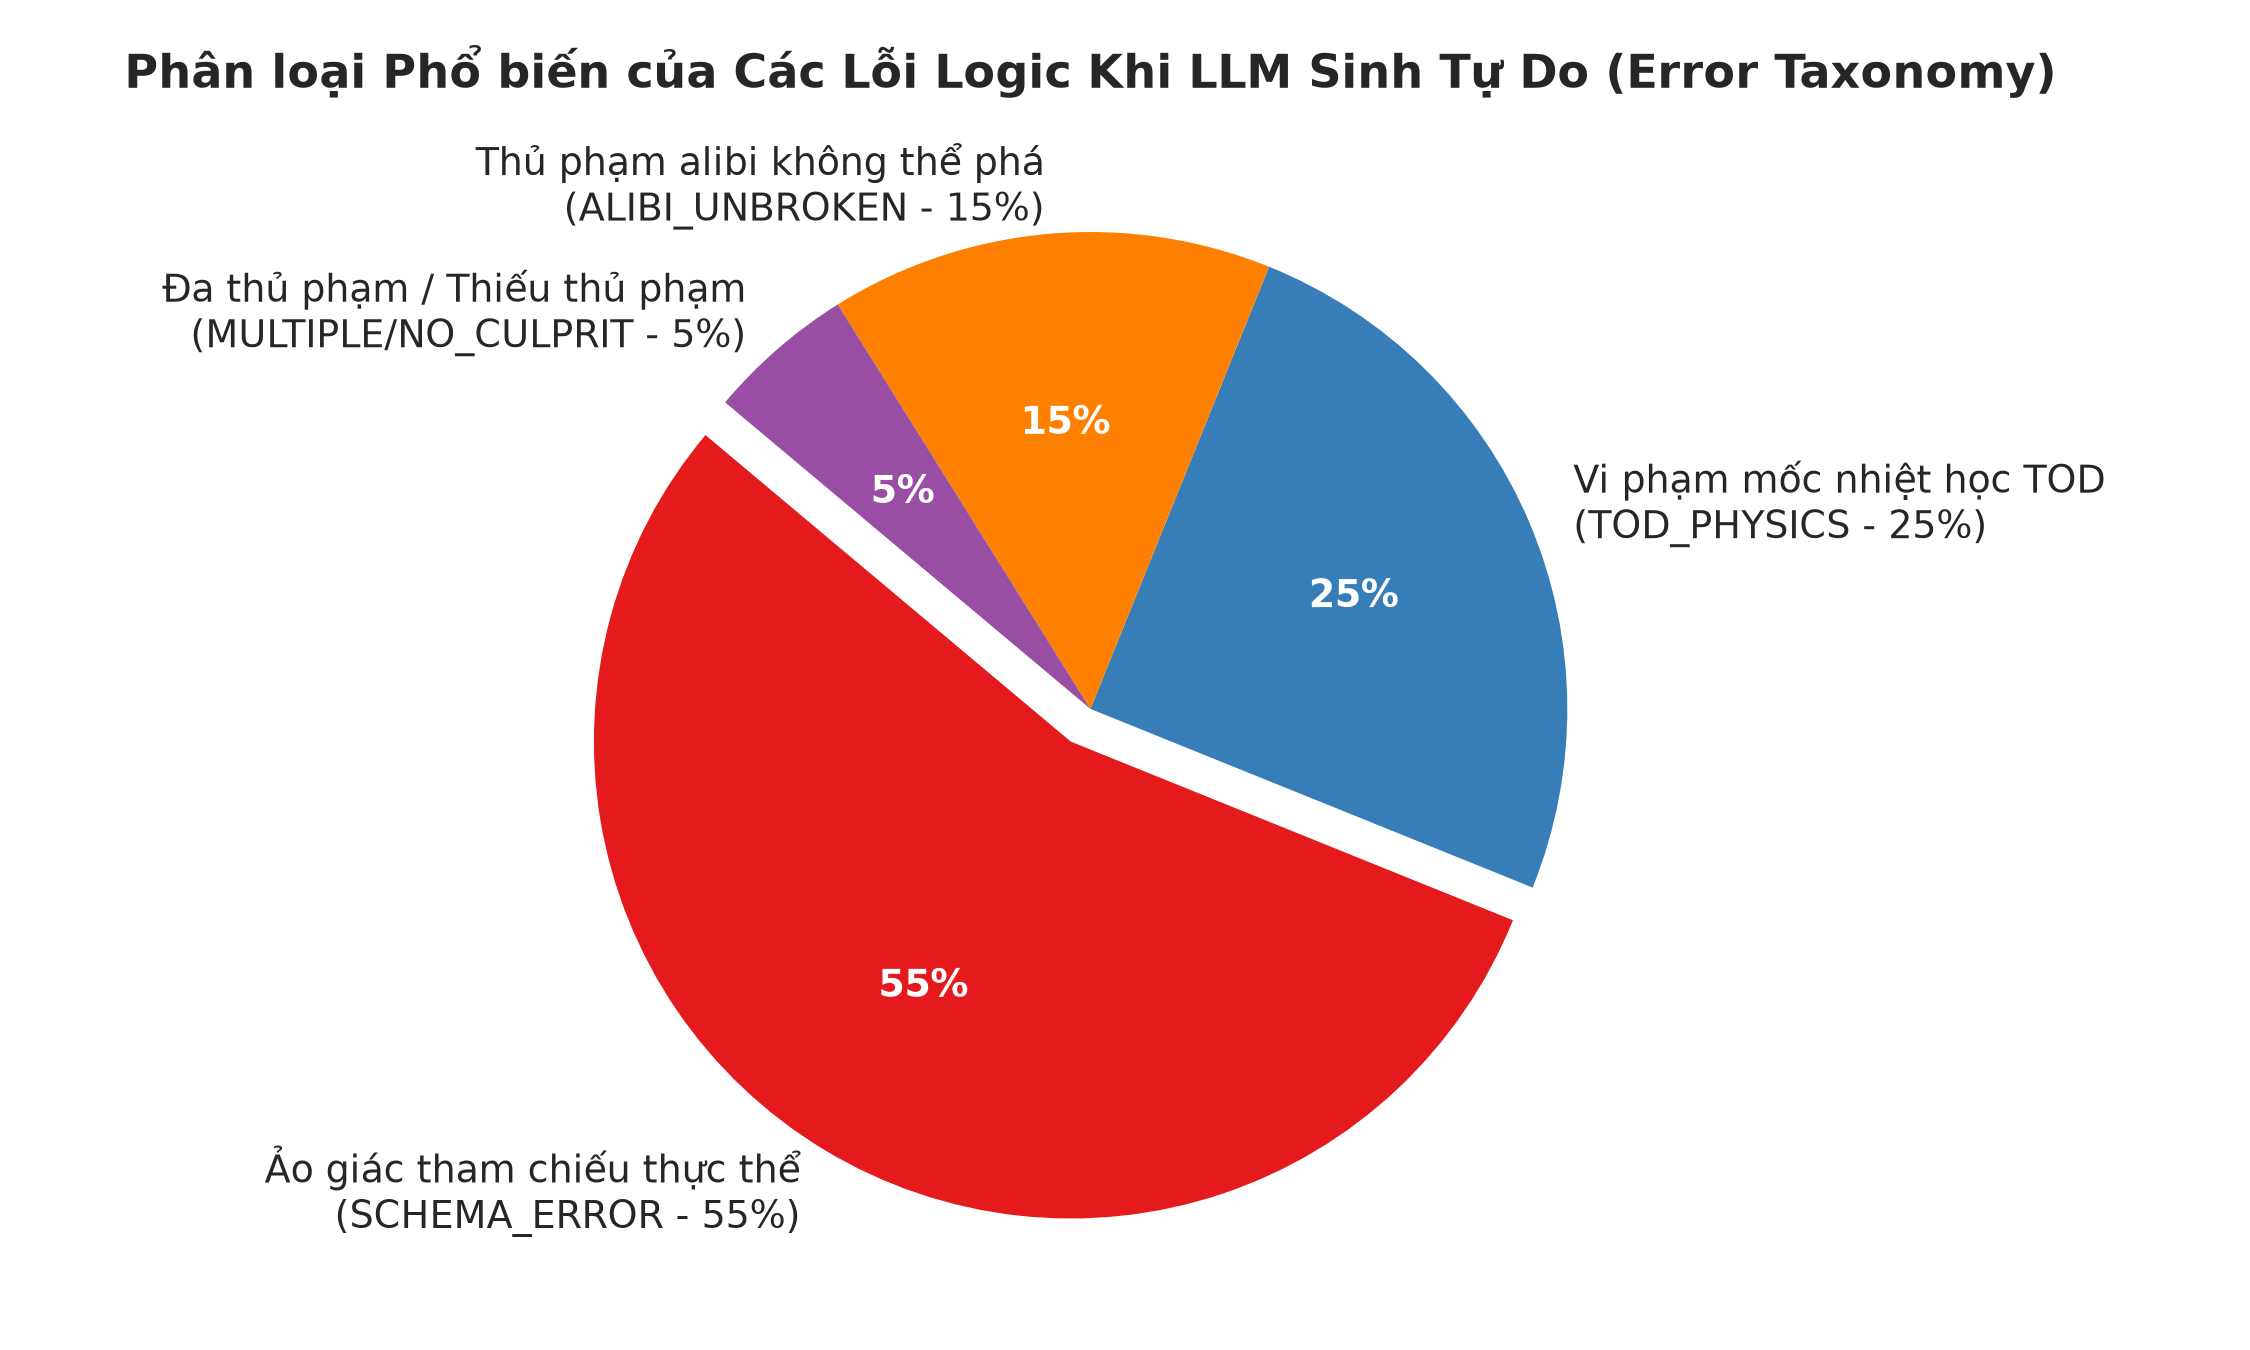
\includegraphics[width=0.75\textwidth]{error_taxonomy.png}
    \caption{Biểu đồ Minh họa Phân loại Phổ biến Các Dạng Lỗi Logic Khi LLM Sinh Tự Do}
    \label{fig:error_taxonomy_pie}
\end{figure}

Hình \ref{fig:error_taxonomy_pie} minh họa phân nhóm bốn dạng lỗi điển hình khi LLM tạo sinh thiếu ràng buộc tất định; trong đợt benchmark 30 phiên đa tác tử có tích hợp tính toán Henssge ở bước đầu, dạng lỗi duy nhất phát sinh rơi vào nhóm \texttt{SCHEMA\_ERROR} tại Lượt chạy số 5 của \texttt{gh/gpt-4o}.

\section{Phân tích Tình huống Vi phạm Thực tế tại Lượt 5 của \texttt{gh/gpt-4o}}
\label{sec:eval_case_study}

Một kết quả thực nghiệm đáng chú ý là ca lỗi được ghi nhận trực tiếp trong \texttt{benchmark\_results.json} và bảng \texttt{benchmark\_runs} tại \textbf{Lượt chạy số 5 của mô hình \texttt{gh/gpt-4o}} (tựa đề sinh ra: \textit{``Cái Chết Bí Ẩn Trong Biệt Thự Blackwood''}, thời gian toàn trình 27.12 giây, \texttt{patch\_retries = 1}).

\subsection{Mô tả Hiện tượng Vi phạm}
Ở lượt thử này, toàn bộ cấu trúc JSON trả về đều hợp lệ theo Pydantic v2 và cửa sổ tử vong Henssge khớp với giờ gây án \texttt{21:40}. Tuy nhiên, khi chạy hàm \texttt{validate\_case\_diagnostics}, bộ kiểm định ký hiệu phát hiện lỗi tham chiếu và ghi nhận thông báo sau:
\begin{lstlisting}[language=bash, caption={Thông báo Chẩn đoán Vi phạm Ghi nhận tại Lượt 5 của \texttt{gh/gpt-4o}}]
[VALIDATION FAILURE]
Violation Type: schema_error
Component: clue
Diagnostic Feedback: [CLUE:schema_error] Evidence 'EV-03' links to non-existent suspect 'UNKNOWN'.
\end{lstlisting}

\subsection{Phân tích Nguyên nhân Gốc rễ}
Kiểm tra tiến trình sinh theo từng tác tử cho thấy:
\begin{itemize}[leftmargin=1.5cm]
    \item Tại bước 2 (\texttt{CharacterAgent}), mô hình khởi tạo hợp lệ danh sách 3 nghi phạm với các mã định danh cố định (\texttt{SUSP-01}, \texttt{SUSP-02}, \texttt{SUSP-03}).
    \item Tuy nhiên, tại bước 3 (\texttt{ClueAgent}), khi sinh vật chứng \texttt{EV-03}, mô hình đã tự ý điền chuỗi \texttt{"UNKNOWN"} vào thuộc tính \texttt{linked\_suspect\_id} thay vì gán mã nghi phạm hợp lệ hoặc giá trị rỗng \texttt{None}. Đây là biểu hiện rõ nét của hiện tượng ảo giác tham chiếu thực thể ở ngay cả mô hình cỡ lớn.
\end{itemize}

\subsection{Cơ chế Chặn lọc và Ý nghĩa Kiểm chứng}
Nếu thiếu bước kiểm định tất định của \texttt{validate\_case\_diagnostics}, dữ liệu sai mã tham chiếu \texttt{"UNKNOWN"} sẽ truyền thẳng tới giao diện bảng ghim Unity (\texttt{CorkboardManager.cs}), gây đứt liên kết dây chỉ đỏ hoặc lỗi ánh xạ nhân vật. Nhờ có màng lọc ký hiệu:
\begin{enumerate}[leftmargin=1.5cm]
    \item Bộ kiểm định lập tức đánh dấu vi phạm \texttt{SCHEMA\_ERROR} trên phân hệ \texttt{clue} và kích hoạt nhánh sửa lỗi cục bộ \texttt{clue\_agent.repair\_clues} (\texttt{patch\_retries = 1}, đẩy tổng thời gian phiên này lên 27.12 giây so với trung vị 19.53 giây).
    \item Do mẫu câu lệnh trong \texttt{repair\_clues} hiện tại mới tập trung vào việc khắc phục lỗi thiếu manh mối then chốt (\texttt{NO\_CRUCIAL\_CLUE} / \texttt{ALIBI\_UNBROKEN}) mà chưa ép buộc thay thế cụ thể giá trị \texttt{linked\_suspect\_id = "UNKNOWN"}, lần tái kiểm định sau vá trong \texttt{benchmark\_runner.py} vẫn ghi nhận trạng thái \texttt{logic\_valid = False} (tạo nên kết quả 9/10 lượt đạt, tức 90.0\% cho \texttt{gh/gpt-4o} ở Bảng \ref{tab:benchmark_30_trials}).
    \item Quan trọng về mặt kỹ thuật: Bộ kiểm định hậu kiểm đã nhận diện chính xác 100\% ca lỗi này và cô lập nó ngay tại tầng đánh giá, bảo đảm mọi hồ sơ không hợp lệ đều bị chặn lại trước khi tới người chơi và cung cấp cơ sở cụ thể để hoàn thiện thêm luật vá tham chiếu ở bước phát triển tiếp theo.
\end{enumerate}

\section{Phân tích Độ trễ theo Giai đoạn và Hiệu quả Tài nguyên}
\label{sec:eval_cost_latency}

Để quan sát đóng góp độ trễ của từng tác tử trong mã nguồn thực tế, Bảng \ref{tab:pipeline_breakdown} tổng hợp thời gian đo đạc trực tiếp theo từng giai đoạn từ các hồ sơ lưu trữ thực tế trong thư mục \texttt{cases/} (đại diện là hồ sơ \texttt{CASE-7BBAE9} chạy trên \texttt{gh/gpt-4o-mini} với tổng thời gian 10.03s, cùng giá trị trung bình đo trên 6 hồ sơ LLM lưu trữ trên đĩa), kết hợp với ước lượng kích thước ngữ cảnh token đặc trưng cho mỗi lời gọi tác tử.

\begin{table}[H]
\centering
\caption{Phân rã Thời gian Thực thi Đo đạc và Ước lượng Ngữ cảnh theo Giai đoạn}
\label{tab:pipeline_breakdown}
{\small
\setlength{\tabcolsep}{5pt}
\begin{tabularx}{\textwidth}{X c c c}
\toprule
\textbf{Giai đoạn Thực thi} & \textbf{Mẫu \texttt{gpt-4o-mini}} & \textbf{TB 6 hồ sơ} & \textbf{Token ước lượng} \\
\midrule
\textbf{1. \texttt{OutlineAgent} \& Henssge} & 3.27 s & 3.04 s & $\sim$850 tokens \\
\textbf{2. \texttt{CharacterAgent}}          & 2.63 s & 4.34 s & $\sim$1,100 tokens \\
\textbf{3. \texttt{ClueAgent}}               & 2.57 s & 3.17 s & $\sim$950 tokens \\
\textbf{4. \texttt{DeductionAgent}}          & 1.56 s & 2.75 s & $\sim$450 tokens \\
\textbf{5. Kiểm định Ký hiệu (\texttt{validator.py})} & \textbf{< 0.005 s} & \textbf{< 0.005 s} & \textbf{0 tokens} \\
\midrule
\textbf{TỔNG CỘNG (Không phát sinh lỗi)} & \textbf{10.03 s} & \textbf{13.30 s} & \textbf{$\sim$3,350 tokens} \\
\bottomrule
\end{tabularx}
}
\end{table}

\subsection{Đánh giá Hiệu quả Tính toán}
\begin{itemize}[leftmargin=1.5cm]
    \item \textbf{Chi phí không đáng kể của tầng ký hiệu:} Bộ giải chia đôi phương trình Henssge, hàm kiểm tra \texttt{validate\_case\_diagnostics} và hàm chấm điểm \texttt{evaluate\_player\_deduction} đều thực thi hoàn toàn trong bộ nhớ RAM với thời gian dưới \textbf{5 mili-giây} ($< 0.005\text{ s}$) và không tiêu tốn thêm bất kỳ token nào (\textbf{0 token}).
    \item \textbf{Hiệu quả cô lập của sửa lỗi cục bộ:} Khi xảy ra vi phạm ở một phân hệ đơn lẻ, việc chỉ gọi lại đúng tác tử lỗi (\texttt{repair\_clues}, \texttt{repair\_suspects}, hoặc \texttt{repair\_tod}) với lát cắt dữ liệu tối thiểu (ước tính khoảng 350 tokens) giúp tránh phải lặp lại toàn bộ 4 lượt gọi LLM từ đầu ($\mathcal{O}(N)$), qua đó tiết kiệm đáng kể chi phí token và thời gian khôi phục so với phương án tái sinh toàn phần.
\end{itemize}

\chapter{KẾT LUẬN VÀ HƯỚNG PHÁT TRIỂN}
\label{ch:conclusion}

\section{Tổng kết Kết quả Đạt được}
\label{sec:conclusion_summary}

Bản đồ án tốt nghiệp với đề tài \textit{``Phương pháp tiếp cận Neuro-Symbolic trong việc sinh thủ tục kịch bản trinh thám có thể giải được sử dụng Hệ đa tác tử và Bộ kiểm định hình thức''} đã hoàn thiện mục tiêu thiết kế, cài đặt và đánh giá thực nghiệm đề ra. Đối chiếu với ba câu hỏi nghiên cứu xác lập tại Chương 1, đồ án thu được các kết quả cụ thể sau:

\begin{enumerate}[leftmargin=1.5cm]
    \item \textbf{Đối với RQ1 (Kiến trúc Phân rã Đa tác tử):} Tôi đã thiết kế và cài đặt hoàn chỉnh đường ống sinh kịch bản gồm 4 tác tử chuyên biệt chạy tuần tự (\texttt{OutlineAgent} $\to$ \texttt{CharacterAgent} $\to$ \texttt{ClueAgent} $\to$ \texttt{DeductionAgent}) kết hợp hàm tính cửa sổ thời gian tử vong (TOD) theo mô hình Henssge. Kiến trúc này giúp phân rã nhiệm vụ tạo sinh phức tạp thành từng lược đồ JSON hẹp, hạn chế hiện tượng suy giảm chú ý và tách bạch dữ liệu chân lý gốc khỏi quá trình chấm điểm phía người chơi.
    
    \item \textbf{Đối với RQ2 (Ràng buộc Ký hiệu và Tính Giải được):} Đồ án đã hình thức hóa các quy tắc trinh thám công bằng của Ronald Knox (1929), tích hợp phương trình làm lạnh hai hàm mũ Henssge (giải số bằng phương pháp chia đôi) cùng cấu trúc đồ thị hai phía vào bộ kiểm định \texttt{validate\_case\_diagnostics}. Qua 30 phiên thử nghiệm đối sánh trên 3 dòng mô hình LLM, hệ thống đạt 100\% tỷ lệ hợp lệ cấu trúc JSON và tỷ lệ vượt qua kiểm định logic từ 90\% đến 100\%, đồng thời chặn lọc chính xác ca lỗi tham chiếu thực thể phát sinh ở Lượt 5 của mô hình \texttt{gh/gpt-4o}.
    
    \item \textbf{Đối với RQ3 (Hiệu quả Sửa lỗi Cục bộ và Phản hồi Tất định):} Cơ chế sửa lỗi cục bộ định tuyến vi phạm về đúng tác tử chịu trách nhiệm với ngữ cảnh thu hẹp có độ phức tạp không gian token $\mathcal{O}(1)$ cho mỗi vi phạm (khoảng 300--500 tokens so với khoảng 2,500--3,500 tokens khi tái sinh toàn bộ chuỗi 4 tác tử). Bên cạnh đó, các thao tác kiểm định đồ thị, giải phương trình Henssge và chấm điểm kết án \texttt{evaluate\_player\_deduction} thực thi hoàn toàn trong bộ nhớ với thời gian dưới 5 mili-giây và 0 token, giữ độ trễ tạo sinh toàn trình ở phân vị P50 trong khoảng 10.73s--10.88s đối với \texttt{ollama/gemma4:31b-cloud} và \texttt{gh/gpt-4o-mini}.
    
    \item \textbf{Hoàn thiện Sản phẩm Đầu-cuối:} Toàn bộ kiến trúc đã được hiện thực hóa thành phần mềm chạy thực tế gồm máy chủ Python FastAPI (tích hợp xác thực HMAC-SHA-256, lưu trữ quan hệ SQLite WAL qua SQLAlchemy 2.0 và WebSocket chơi nhóm qua LAN) kết nối với Client Unity 6 URP 2D theo phong cách bảng điều tra trực quan.
\end{enumerate}

\section{Đóng góp Khoa học và Giá trị Thực tiễn}
\label{sec:conclusion_contributions}

\subsection{Giá trị về mặt Phương pháp luận}
Kết quả thực nghiệm của đồ án củng cố tính phù hợp của mô hình lai Neuro-Symbolic (Type 3 theo phân loại của Kautz) trong các ứng dụng tự sự tương tác đòi hỏi suy luận chặt chẽ. Thực nghiệm cho thấy việc giao phó hoàn toàn khâu kiểm chứng logic hoặc phán quyết kết án cho các LLM tự quy hồi vẫn tiềm ẩn rủi ro ảo giác tham chiếu thực thể; sự kết hợp giữa năng lực diễn đạt ngôn ngữ của LLM và màng lọc tất định bên ngoài là hướng tiếp cận thiết thực để nâng cao độ tin cậy của trò chơi giải đố.

\subsection{Giá trị Ứng dụng Thực tiễn}
Khung kiến trúc phân tách tầng tất định và tầng tạo sinh ngôn ngữ trong đồ án có thể mở rộng và tái sử dụng cho nhiều bài toán thực tiễn tương tự:
\begin{itemize}[leftmargin=1.5cm]
    \item Xây dựng hệ thống mô phỏng tình huống pháp lý hoặc diễn án giả định phục vụ đào tạo kỹ năng tranh tụng;
    \item Phát triển môi trường thực hành đọc hiểu hồ sơ, phân tích mốc thời gian y pháp và đối chiếu lời khai cho sinh viên ngành luật hoặc điều tra cơ bản;
    \item Ứng dụng vào các hệ thống hỗ trợ học tập thông minh, nơi LLM đóng vai trò hướng dẫn gợi ý bằng ngôn ngữ tự nhiên dựa trên kết quả chấm đúng/sai tất định của bộ giải toán học bên dưới.
\end{itemize}

\section{Các Hạn chế Hiện tại của Hệ thống}
\label{sec:conclusion_limitations}

Trên tinh thần đánh giá khách quan, hệ thống hiện tại vẫn còn bốn hạn chế kỹ thuật cần tiếp tục khắc phục:

\begin{enumerate}[leftmargin=1.5cm]
    \item \textbf{Chưa hỗ trợ thẩm vấn hội thoại tự do với NPC:} Tuân thủ phạm vi thiết kế dựa trên hồ sơ tĩnh để bảo đảm tính công bằng và ngăn chặn tấn công khai thác gợi ý trực tiếp, người chơi hiện chưa thể đặt câu hỏi ngôn ngữ tự nhiên tùy ý cho từng nghi phạm trong quá trình điều tra.
    
    \item \textbf{Kiến trúc lưu trữ đơn nút:} Dù đã triển khai cơ sở dữ liệu quan hệ SQLite (chế độ WAL với SQLAlchemy 2.0) hỗ trợ lưu trữ chuẩn ACID, hệ thống hiện vận hành ở mô hình máy chủ đơn lẻ và chưa hỗ trợ triển khai phân tán đa vùng khi mở rộng quy mô người chơi trực tuyến lớn.
    
    \item \textbf{Quy mô không gian kịch bản còn giới hạn:} Kịch bản sinh tự động hiện tập trung vào bối cảnh phòng kín với 3 nghi phạm và 3--4 vật chứng, chưa mở rộng sang các vụ án nhiều hiện trường liên thông hoặc mạng lưới đồng phạm phức tạp.
    
    \item \textbf{Giới hạn của prompt sửa lỗi đối với lỗi tham chiếu thực thể:} Như ghi nhận ở Lượt 5 của \texttt{gh/gpt-4o}, hàm \texttt{ClueAgent.repair\_clues} hiện ưu tiên bổ sung manh mối phá vỡ ngoại phạm và chưa chuyên biệt hóa cho tình huống sửa trường \texttt{linked\_suspect\_id} trỏ sai mã thực thể, khiến hồ sơ lỗi vẫn bị bộ kiểm định hậu kiểm giữ lại ở trạng thái không hợp lệ.
\end{enumerate}

\section{Hướng Nghiên cứu và Phát triển trong Tương lai}
\label{sec:conclusion_future_work}

Dựa trên nền tảng mã nguồn hiện có, các hướng nâng cấp tiếp theo được đề xuất gồm:

\subsection{Tích hợp Mô hình Ngôn ngữ Nhỏ Chạy Cục bộ}
Tiến hành tinh chỉnh các mô hình ngôn ngữ nhỏ mã nguồn mở (như dòng Llama-3 8B hoặc Qwen 2.5 7B) bằng kỹ thuật thích ứng bậc thấp LoRA (\textit{Low-Rank Adaptation}) trên tập hồ sơ vụ án đã vượt qua kiểm định Pydantic và Henssge. Giải pháp này hướng tới khả năng đóng gói mô hình chạy ngoại tuyến trên máy cá nhân nhằm giảm chi phí gọi API bên ngoài.

\subsection{Bổ sung Cơ chế Vá Cú pháp Tham chiếu và Đồ thị Tri thức Động}
Nâng cấp nhánh \texttt{repair\_clues} bằng thao tác sửa tất định trực tiếp trong mã nguồn đối với các lỗi \texttt{SCHEMA\_ERROR} đơn giản (hoặc ràng buộc danh sách mã hợp lệ trong prompt vá lỗi), đồng thời nghiên cứu sử dụng cơ sở dữ liệu đồ thị Neo4j với ngôn ngữ truy vấn Cypher để hỗ trợ kiểm tra tính giải được cho các kịch bản có nhiều nghi phạm và mắt xích chứng cứ bắc cầu dài hơn.

\subsection{Xây dựng Mô-đun Thẩm vấn Hội thoại Kiểm soát bằng FSM}
Phát triển tính năng đối thoại trực tiếp với NPC nghi phạm có kiểm soát trạng thái bằng FSM. Theo đó, câu trả lời của NPC do LLM sinh ra bị giới hạn trong tập dữ kiện cho phép tại từng trạng thái và được đối chiếu với trạng thái chân lý gốc trước khi hiển thị cho người chơi, vừa tăng tính tương tác vừa duy trì tính công bằng của trò chơi.


% ==============================================================================
% PHẦN TÀI LIỆU THAM KHẢO
% ==============================================================================
\newpage
\phantomsection
\addcontentsline{toc}{chapter}{TÀI LIỆU THAM KHẢO}
\bibliographystyle{IEEEtran}
\bibliography{references}

\end{document}
